\setcounter{chapter}{4}
\chapter{Introducción al Modelo y gestión de datos}
Este capítulo presenta el modelo y los criterios de gestión de datos de la solución propuesta por Synaptix para la Marina y Club Náutico Bahía Panitao S.A. Su propósito es relacionar los hechos operacionales con sus antecedentes contractuales, administrativos y ambientales, conservando la evidencia necesaria para reconstruir cada actuación. El diseño considera las condiciones de conectividad del puerto y las exigencias de protección de datos personales, especialmente de menores de edad, establecidas en las bases del caso (Pontificia Universidad Católica de Valparaíso [PUCV], 2026c, caps.~10 y~15).

El diagnóstico, la volumetría y las restricciones del Subdocumento 2 fundamentan las necesidades de información. El Subdocumento 3 delimita las capacidades y los procesos que generan o utilizan esos datos, mientras el Subdocumento 4 establece los dominios responsables y su distribución entre nube, recinto y terreno. La relación entre requerimientos y diseño toma como referencia el Formulario T-12; la correspondencia con las tecnologías de almacenamiento e integración se apoya en el Formulario T-11.

El desarrollo se organiza en cuatro apartados. La sección 5.1 define los dominios, las entidades, sus relaciones y la gestión de datos maestros. La sección 5.2 aborda la persistencia, la consistencia, la sincronización, la separación entre operación y analítica, y las políticas de calidad, protección y ciclo de vida. La sección 5.3 trata la migración, el saneamiento y la conciliación de los antecedentes históricos. Finalmente, el apartado~5.4 aborda la optimización del almacenamiento y las consultas según la volumetría y las necesidades de actualización del caso. Los anexos reúnen el detalle de apoyo, incluido el diccionario de datos del Anexo A5.1.

%---------------------------------------------
\newpage
\section{Modelo} %5.1
El modelo de datos establece qué información necesita conservar la solución, qué significa cada entidad y cómo se relaciona con los procesos del puerto. Se organiza según los nueve dominios canónicos del Subdocumento 4 y mantiene la relación con las capacidades funcionales del Subdocumento 3. Cada entidad conserva una identidad y una responsabilidad definidas, incluso cuando sus datos se utilizan en distintos procesos o emplazamientos.

Las relaciones y reglas del modelo permiten distinguir situaciones con consecuencias diferentes para el negocio: una asignación contractual y una ocupación física, una solicitud de retiro y una entrega efectiva de un alumno, o una medición y un consumo validado. Estas diferencias orientan la representación de estados, vigencias y evidencias, y permiten identificar qué antecedentes respaldan una decisión y quién tiene autoridad para confirmarla.

La sección 5.1.1 presenta los dominios y las entidades compartidas; la sección 5.1.2 desarrolla sus relaciones y reglas mediante figuras por dominio; y la sección 5.1.3 aborda la identificación, actualización y conciliación de datos maestros. El detalle por atributo corresponde al diccionario del Anexo A5.1, cuya especificación debe incluir nombre, tipo, dominio de valores, obligatoriedad, propietario y sensibilidad, conforme al requisito RT-05.01 de las Bases Técnicas Transversales (PUCV, 2026b). Esta definición proporciona la referencia común para la gestión, la migración y la optimización de datos desarrolladas en los apartados siguientes.

\subsection{Dominios y entidades} %5.1.1
El modelo de información de Synaptix organiza los antecedentes necesarios para gestionar embarcaciones, controlar la participación de alumnos, coordinar los servicios del puerto y respaldar sus efectos administrativos y ambientales.
%Se construye a partir del diagnóstico del SD2, del alcance funcional del SD3 y de la arquitectura del SD4.
Las entidades y reglas que siguen constituyen el diseño propuesto para estas secciones, no representan datos reales ya migrados ni controles implementados. Su finalidad es eliminar registros contradictorios, conservar la evidencia de cada actuación y establecer una responsabilidad clara sobre cada dato. %(PUCV, 2026a, RT-05.01, RT-05.03 y RT-05.09, pp. 11-12; Synaptix, 2026a, sec. 2.5 y anexos A2.1-A2.5).

La organización adopta los nueve dominios canónicos definidos en SD4, tabla 4.2 y decisión DA-03: operación marítima; clientes y contratos; escuela náutica; varadero y contratistas; combustible; ambiente y consumos; finanzas y cobranza; infraestructura; auditoría y seguridad. Los doce códigos funcionales NAV, ALE, ESC, AMA, VAR, CTR, AMB, CON, BOY, FAC, ADM y AUT se conservan para la trazabilidad de los requerimientos. Un módulo funcional expresa una capacidad del servicio, un dominio identifica la responsabilidad sobre sus datos y reglas. Por esta razón, no se necesita definir una correspondencia uno a uno, ni una base de datos independiente para cada código.
%(Synaptix, 2026b, sec. 3.3.2, pp. PDF 18-20; Synaptix, 2026c, sec. 4.1, pp. PDF 5-7).

La Tabla%~\ref{tab:nombre}
5.1 relaciona la nomenclatura de los catálogos con el dominio y la agrupación de ejecución descrita en el SD4. El mapa conserva las capacidades del SD3 y distingue su decomposición funcional de la distribución arquitectónica adoptada para este modelo.

\begingroup
\setlength{\tabcolsep}{3pt}

\begin{longtable}{@{}
    L{.34\textwidth}
    L{.33\textwidth}
    L{\dimexpr.33\textwidth-12pt\relax}
@{}}
    \caption{Correspondencia funcional y propiedad de datos}
    \label{tab:sd5_correspondencia_dominios}\\ \hline
    \EncabezadoTabla{Dominio canónico} &
    \EncabezadoTabla{Códigos funcionales} &
    \EncabezadoTabla{Agrupación SD4} \\ \hline \endfirsthead
    \hline
    \EncabezadoTabla{Dominio canónico} &
    \EncabezadoTabla{Códigos funcionales} &
    \EncabezadoTabla{Agrupación SD4} \\ \hline \endhead

    Operación marítima & NAV; AMA; BOY & Núcleo Operacional \\ \addlinespace \hline
    Clientes y contratos & ADM; AMA; AUT & Núcleo Administrativo \\ \addlinespace \hline
    Escuela náutica & ESC; AUT; CTR (retiro) & Núcleo Operacional \\ \addlinespace \hline
    Varadero y contratistas & VAR; CTR; AUT & Núcleo de Servicios \\ \addlinespace \hline
    Combustible & CON (despacho) & Núcleo de Servicios \\ \addlinespace \hline
    Ambiente y consumos & AMB; CON (medición) & Núcleo de Servicios \\ \addlinespace \hline
    Finanzas y cobranza & FAC; AUT & Núcleo Administrativo \\ \addlinespace \hline
    Infraestructura & AMA; BOY; CON; VAR & Núcleo Operacional \\ \addlinespace \hline
    Auditoría y seguridad & ADM; ESC; AUT; todos & Proceso especializado \\ \addlinespace \hline
\end{longtable}
\endgroup

Los cruces de la tabla fueron definidos de manera intencional, a continuación se describen las observaciones obtenidas de la tabla:
\begin{itemize}
    \item \textbf{AMA} participa en tres dominios: Infraestructura describe el lugar físico, Clientes y contratos mantiene su asignación contractual y Operación marítima determina la ocupación en base a hechos y evidencias.
    \item \textbf{CON} diferencia el despacho de combustible con el agua y energía.
    \item \textbf{BOY} combina inventario e inspecciones de infraestructura con observaciones operacionales.
    \item \textbf{ALE} se establece mediante el servicio especializado de notificaciones: el dominio de origen decide el contenido del aviso, y el servicio conserva destinatarios, intentos y acuses.
    \item \textbf{AUT} es un canal de acceso: una operación iniciada en el portal mantiene la identidad y las reglas de la entidad de negocio que modifica.
\end{itemize}

Las entidades compartidas por referencia son Persona, Organización, Embarcación, Contrato y Activo. Persona identifica al individuo y Organización a la entidad jurídica o institucional, sus funciones se representan mediante vínculos vigentes evitando crear una persona distinta por cada rol. Embarcación conserva su identificador aunque cambien el armador, el contrato o su ubicación. Contrato preserva las partes, las versiones y el período de validez. Activo identifica la infraestructura física; Amarra, Boya, Medidor y los elementos de fondeo mantienen sus características específicas. Una cuenta de acceso es una identidad de autenticación vinculada con una persona, no un sustituto del padrón de clientes, alumnos o trabajadores.

La Figura~\ref{fig:entidades_responsabilidades} presenta las relaciones estructurales que permiten conectar la custodia física con sus antecedentes personales y contractuales. Las cardinalidades 1, 0..1, 0..N y 1..N significan, respectivamente, uno, cero o uno, cero o varios, y uno o varios. Las referencias se reconocen por el sufijo de dominio: CC, Clientes y contratos; INF, Infraestructura; OM, Operación marítima; EN, Escuela náutica; VC, Varadero y contratistas; CO, Combustible; AC, Ambiente y consumos; FC, Finanzas y cobranza; AS, Auditoría y seguridad. Estas siglas se usan únicamente para leer las figuras y no sustituyen los códigos RF/RNF.

\begin{figure}[htbp]
    \centering
    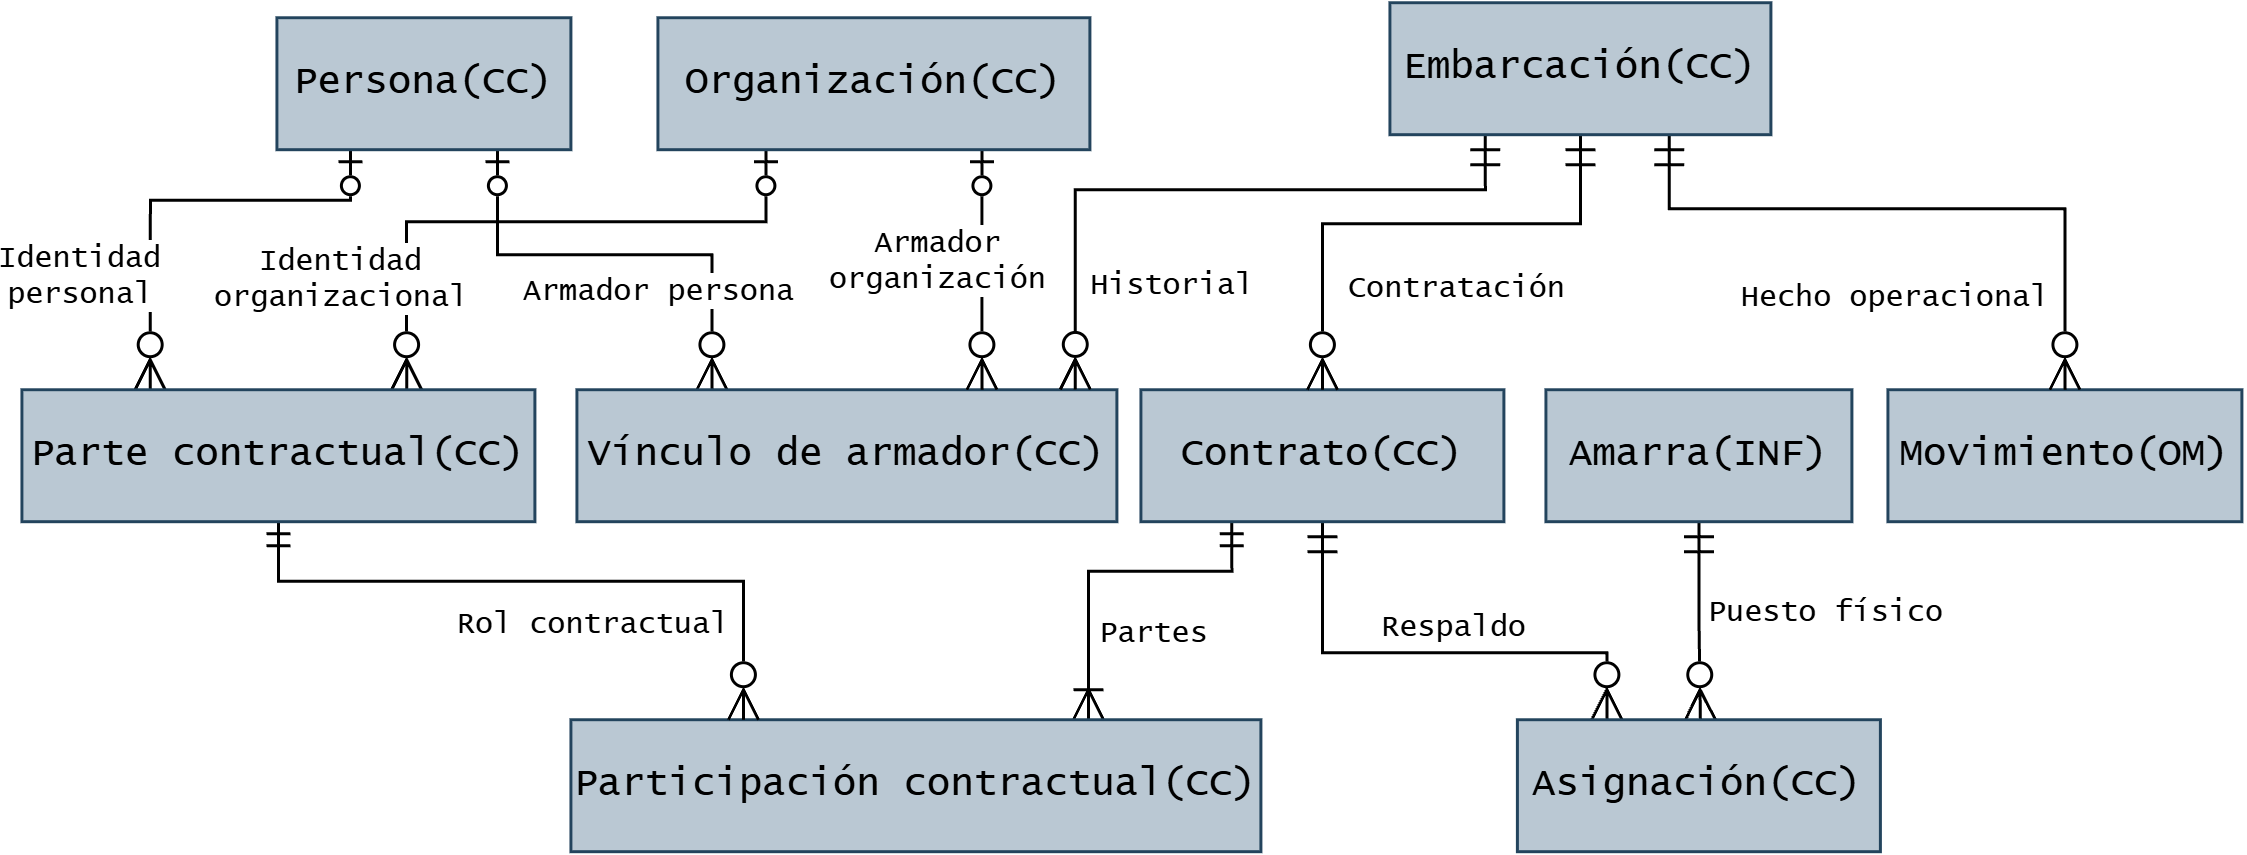
\includegraphics[width= \linewidth]{figuras/F5_1.png}
    \caption{Entidades compartidas y sus responsabilidades}
    \label{fig:entidades_responsabilidades}
    \FuenteFigura{Modelo de datos de Synaptix; dominios y relaciones descritos en esta sección.}
\end{figure}

La Figura~\ref{fig:entidades_responsabilidades} distingue la identidad de una persona de la de una organización y muestra cómo participan en las relaciones del puerto sin confundirse entre sí. Parte contractual referencia exactamente una de esas identidades; Participación contractual registra el rol con que interviene en un contrato. Vínculo de armador conserva, de manera independiente, quién ejerce ese rol respecto de una embarcación y durante qué período. Cada vínculo identifica una persona o una organización, evitando registrar ambas como titulares indistintos de un mismo vínculo.

Asignación relaciona el contrato con la amarra y el intervalo autorizado, mientras Movimiento conserva el hecho operacional de la embarcación. El movimiento no modifica por sí solo el contrato, y la asignación contractual no acredita por sí sola la presencia física. Esta figura ofrece una vista transversal de identidades y relaciones compartidas; los sufijos de las entidades identifican sus dominios propietarios y las figuras siguientes desarrollan sus reglas específicas.

Una asignación vigente no garantiza la presencia física y una señal de presencia no identifica por sí sola al ocupante. Del mismo modo, el cierre declarado de un plan no sustituye la confirmación operacional de regreso. Mantener estas diferencias evita que un único campo de estado mezcle derechos contractuales, observaciones y hechos de seguridad. El mismo principio se aplica a asistencia y retiro, lectura y consumo validado, hecho facturable y documento contable, envío y acuse.

La responsabilidad sobre un dato permanece en su dominio aunque existan copias operacionales o proyecciones de consulta. Según DA-05 y DA-06, los demás dominios acceden mediante contratos o eventos y no modifican tablas ajenas. Los maestros contractuales se administran en nube, y los hechos producidos en el recinto o en terreno conservan su origen y se incorporan mediante el Runtime Operacional de Borde y la sincronización. Las proyecciones indican versión y fecha de actualización. La contabilidad externa mantiene autoridad sobre documentos tributarios, pagos y saldos; Synaptix conserva hechos facturables, respuestas y copias verificables para consulta y conciliación.
%(Synaptix, 2026c, sec. 4.1, pp. PDF 8-9).

La separación por dominio y los identificadores compartidos se mantienen tanto en PostgreSQL como en las copias operacionales locales y en los documentos asociados. Se toma como referencia la persistencia elegida en SD4, DA-08, y los permisos locales de DA-16 y DA-19. Esta sección define significado y propiedad. La justificación del motor, las garantías de consistencia, la sincronización y el ciclo de vida se desarrollan en 5.2. El detalle de atributos se incorpora en el diccionario A5.1.


\subsection{Modelo de datos por dominio} %5.1.2
El modelo lógico se organiza en entidades identificables, relaciones con cardinalidades explícitas y estados que solo pueden cambiar a partir de un hecho verificable. Para facilitar su lectura, los diagramas se presentan separados por dominio.

Cada recuadro identifica una entidad del modelo y cada conexión representa una asociación entre entidades. Las cardinalidades de los extremos indican cuántos registros pueden participar en esa asociación. Por ejemplo, una relación con \texttt{1} junto a Contrato y \texttt{0..N} junto a Asignación expresa que cada asignación pertenece a un contrato, mientras un contrato puede mantener ninguna o varias asignaciones a lo largo de su historia. Esa multiplicidad no autoriza usos simultáneos incompatibles: las restricciones de vigencia y concurrencia se establecen en las reglas del dominio.

Las figuras presentan las asociaciones principales de cada dominio y sus referencias compartidas. Una entidad conserva el mismo significado, identificador y propietario en todas las vistas en que aparece; su repetición no crea otra entidad ni transfiere la autoridad del dato. Las reglas de exclusión, conciliación y cierre se explican junto a la figura porque una cardinalidad no representa todas las condiciones del negocio. El detalle por atributo y las asociaciones complementarias deben documentarse de manera consistente en A5.1.

Todas las entidades poseen una clave primaria estable, denominada \texttt{id}. Para las identidades creadas por software, se propone utilizar UUID v4. El identificador se genera una sola vez por operación y se conserva durante sus reintentos. Esta propuesta concreta el uso de identificadores globales definido en SD4 y apoya la idempotencia establecida en SD3.

Los identificadores externos (matrícula de una nave, el folio contable, el código de un medidor o un documento de identidad) se conservan como claves alternativas, junto con su emisor y ámbito de unicidad. Si no se dispone de un documento verificado, su ausencia se registra como dato no acreditado.

Las referencias entre entidades de un mismo dominio se validan mediante integridad referencial. Las referencias a otros dominios se verifican mediante el contrato del dominio correspondiente o una proyección autorizada de sus datos. Estas referencias no habilitan consultas directas a tablas ajenas.

Los intervalos incluyen el instante de inicio y excluyen el de término. Mientras un vínculo siga vigente, su intervalo permanece sin fecha de término.

Los instantes de los eventos se almacenan en UTC y se muestran en la zona horaria operacional correspondiente. Se distingue entre el momento en que ocurrió un evento y el momento en que fue recibido. Los importes y las mediciones se representan con precisión decimal y una unidad explícita. Además, todo cambio relevante conserva su versión, responsable y motivo.

Cada evento utiliza el sobre de metadatos definido en SD4, compuesto por los campos \texttt{eventId}, \texttt{eventType}, \texttt{schemaVersion}, \texttt{aggregateId}, \texttt{aggregateSequence}, \texttt{occurredAt}, \texttt{recordedAt}, \texttt{source}, \texttt{actor}, \texttt{correlationId}, \texttt{causationId} y \texttt{payload}. La secuencia de eventos tiene validez dentro de la autoridad de su agregado; no se presupone un contador global fiable entre dispositivos desconectados.
%(Synaptix, 2026b, §3.4.2, p. PDF 22; Synaptix, 2026c, §4.1, pp. PDF 8-9).

El registro de negocio y su evento de salida se guardan en una misma transacción local al dominio. Al recibir un evento, la bandeja de entrada utiliza eventId para detectar duplicados y registra el efecto junto con su procesamiento.

Si se recibe una clave ya registrada con un contenido distinto, se conserva como un conflicto. No se acepta silenciosamente como una nueva operación. Las discrepancias mantienen ambos antecedentes y el registro de su resolución: guardar y sincronizar la evidencia no autoriza, por sí solo, el cambio disputado.

Estas reglas concretan DA-05 y DA-06 y distinguen la entrega de mensajes de la ejecución de sus efectos una sola vez.

En los siguientes diagramas por dominio, el azul claro identifica las entidades propias del dominio; el gris claro, las referencias a entidades de otros dominios; el verde claro distingue las entidades del servicio compartido de notificaciones.

\subsubsection{Clientes y contratos}
Este dominio mantiene Persona, Organización, Parte contractual, Representación, Vínculo de armador, Embarcación, Contrato, Versión de contrato, Asignación, Reserva, Solicitud de espera y Tarifa versionada. Parte contractual referencia exactamente una Persona o una Organización. Los campos determinantes son la vigencia y función del vínculo; emisor e identificador de la nave; período, estado y partes del contrato; amarra y período de asignación; y regla de compatibilidad y tarifa aplicadas. Contactos, representaciones y condición de socio tienen vigencia y origen verificable.

La Figura~\ref{fig:clientes_contratos} separa identidad, titularidad y uso contractual. Las partes se vinculan a cada contrato mediante participación contractual, que distingue titular, representante y otras funciones admitidas. Las versiones documentales conservan aceptación y evidencia de firma sin sustituir el identificador del contrato.

\begin{figure}[htbp]
    \centering
    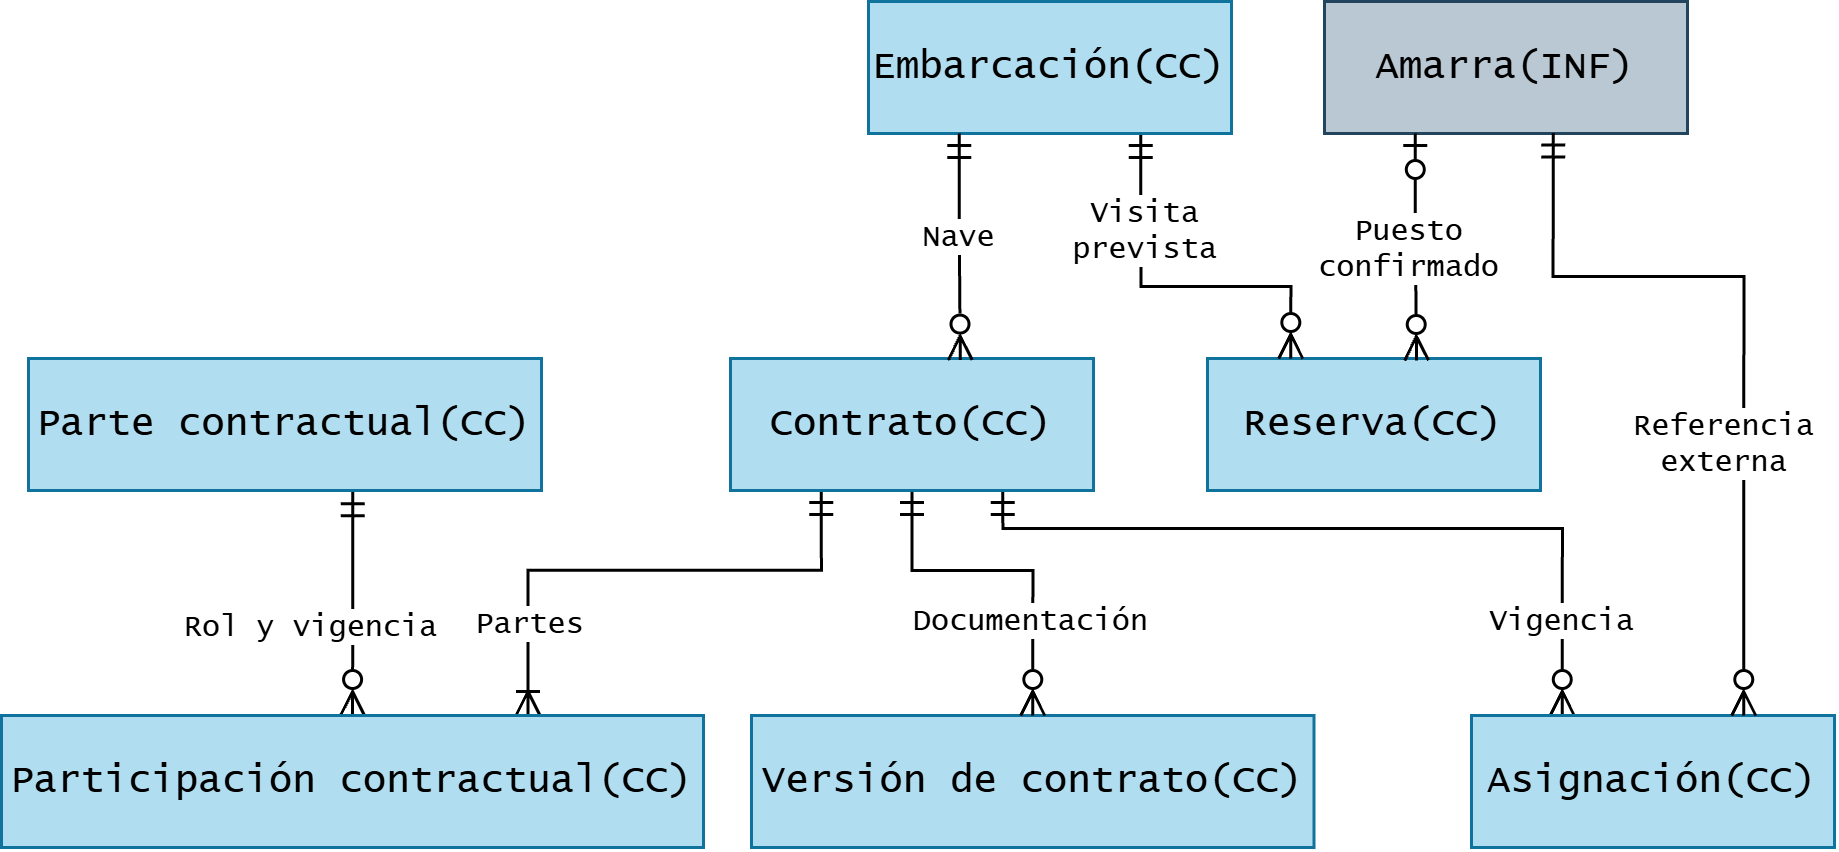
\includegraphics[width=0.8 \linewidth]{figuras/F5_2.png}
    \caption{Clientes, contratos y asignaciones}
    \label{fig:clientes_contratos}
    \FuenteFigura{Modelo de datos de Synaptix; dominios y relaciones descritos en esta sección.}
\end{figure}

La relación entre contrato y asignación ayuda a mantener su historia sin interpretar que una embarcación ocupa físicamente la amarra durante toda la vigencia contractual. Esa condición se obtiene de Operación marítima. Una reserva comienza como 'solicitada' y puede avanzar a 'confirmada', 'atendida', 'cancelada' o 'vencida', su confirmación requiere compatibilidad, período y autorización operacional del puesto. Las asignaciones y reservas confirmadas no pueden comprometer simultáneamente un mismo recurso para usos incompatibles.

La autoridad local registra la autorización operacional de puesto antes de confirmar el resultado comercial. El portal pide esa autorización y, durante una desconexión, el recinto conserva la capacidad de recibir embarcaciones y asignarles amarra. La llegada sin reserva o prepago origina una Recalada con los antecedentes disponibles; posteriormente se vincula con el responsable de pago y el hecho facturable. La formalización contractual mantiene su autoridad en nube, conforme a SD4, y la continuidad local responde a C07 RT-03.10. La lista de espera conserva fecha de ingreso, compatibilidad, oferta, respuesta y vencimiento, junto con la versión de la política utilizada.

Este dominio pertenece al Núcleo Administrativo y distribuye versiones de consulta autorizadas al recinto. Los eventos \texttt{ContratoActualizado}, \texttt{AsignaciónModificada} y \texttt{ContactoActualizado} comunican cambios a los consumidores definidos en SD4. El diseño desarrolla los requerimientos de administración, amarras y autoatención vinculados con RF-ADM-01/04 y RF-AUT-02/03, además de DEC-09 a DEC-11 y RN-07 a RN-09 de los anexos del SD2. El contrato de autorización local de puesto debe quedar reflejado en las interfaces y en la disponibilidad funcional del SD4.

\subsubsection{Operación marítima}
Operación marítima reúne los hechos que permiten determinar dónde se encuentra una embarcación y qué evidencias respaldan ese estado. Recalada identifica una permanencia en el recinto; Salida, un episodio de navegación; y Movimiento registra salida, regreso u otro hecho operacional con instante, lugar, informante y registrador. Confirmación operacional conserva quién comprobó el hecho y mediante qué evidencia. Estas entidades permiten reconstruir la operación aún cuando el registro inicial se realice desde un dispositivo sin conexión.

El Plan de navegación conserva patrón, itinerario declarado, retorno previsto, contactos y consentimiento aplicable. Sus cambios se registran mediante Versión de plan. Persona a bordo y Legajo de zarpe relacionan a los participantes con los antecedentes preparados para el trámite, conservando la versión de los documentos utilizada. Evidencia de ocupación recopila observaciones, movimientos confirmados, declaraciones y señales instrumentales. Estado operacional conserva la conclusión y Sustento de estado identifica las evidencias y la versión de regla que la produjo. La Figura~\ref{fig:operacion_maritima} presenta las asociaciones principales de navegación, confirmación y sustento operacional.

\begin{figure}[htbp]
    \centering
    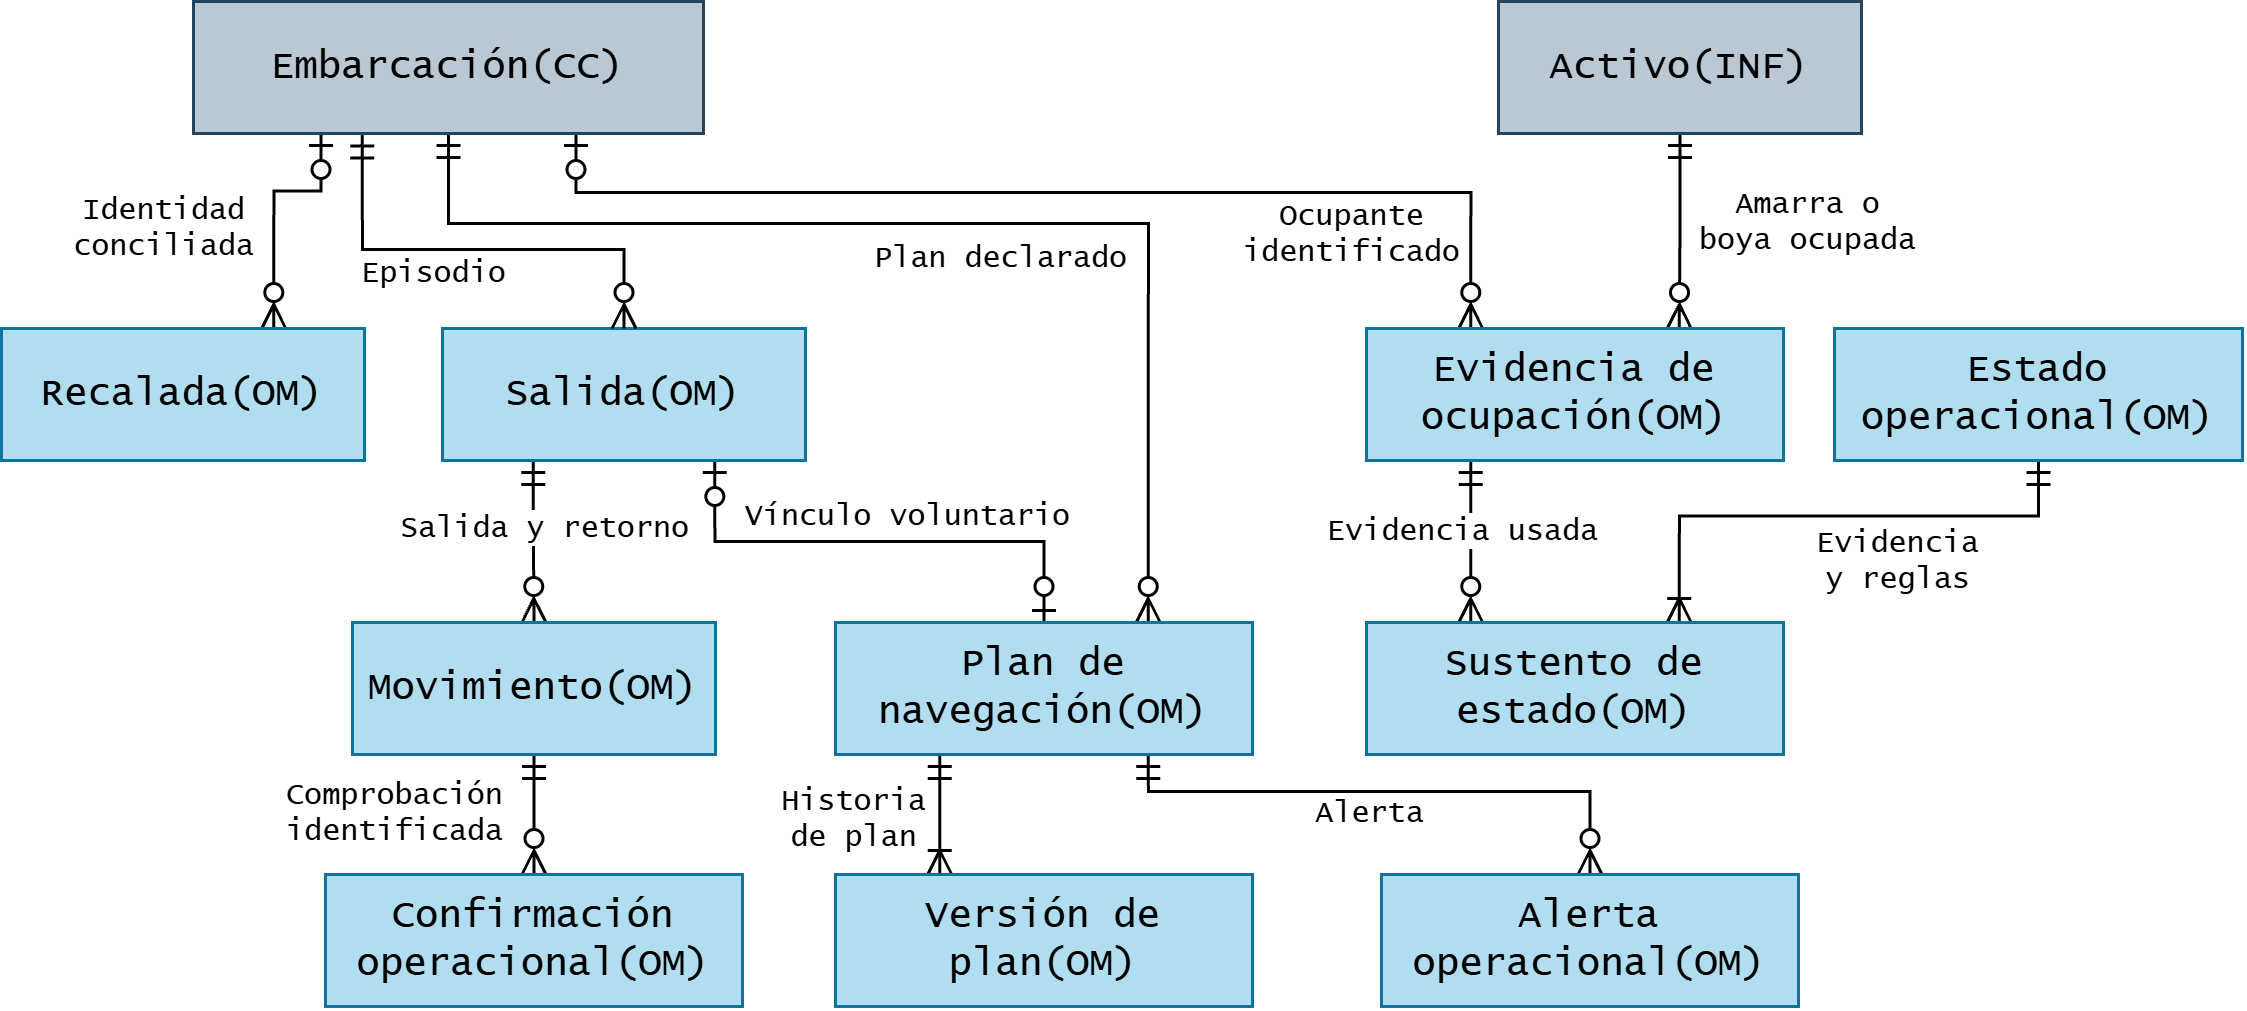
\includegraphics[width= \linewidth ]{figuras/F5_3.png}
    \caption{Navegación, confirmación y evidencia operacional}
    \label{fig:operacion_maritima}
    \FuenteFigura{Modelo de datos de Synaptix; dominios y relaciones descritos en esta sección.}
\end{figure}

La Figura~\ref{fig:operacion_maritima} separa el movimiento informado de su comprobación operacional. Confirmación operacional conserva la actuación que verifica un hecho. Su ausencia mantiene ese hecho pendiente de confirmación, conforme a las reglas del dominio. Versión de plan conserva la historia del Plan de navegación y pertenece a Operación marítima. Esta versión no corresponde a una modificación del contrato comercial ni se registra como participación contractual.

La evidencia de ocupación referencia un Activo de Infraestructura que, en esta asociación, debe corresponder a una Amarra o una Boya. Utilizar su identidad común permite reconocer el lugar observado sin crear una entidad adicional denominada Amarra--Boya. La referencia de embarcación puede permanecer pendiente mientras se concilia una recalada o una observación, conservando sus antecedentes originales. Sustento de estado vincula las evidencias utilizadas con la conclusión operacional y la versión de la regla aplicada. La figura representa esta cadena principal; Persona a bordo y Legajo de zarpe conservan el tratamiento descrito en el texto y deben quedar relacionados en el modelo detallado de A5.1.

La asociación entre Salida y Plan es opcional, una embarcación puede salir sin plan voluntario y un plan puede existir antes de una salida efectiva. El estado de la embarcación distingue en recinto confirmado, salida confirmada, regreso pendiente y discrepancia. El estado del puesto distingue libre verificado, ocupado identificado, ocupado no identificado e indeterminado. La disponibilidad contractual y las restricciones administrativas se consultan como antecedentes adicionales.

El regreso se confirma cuando el marinero observa a la embarcación amarrada en condición segura, la guardia puede registrar lo informado por radio, identificando tanto al informante como al registrador. El armador puede declarar el cierre de su plan, pero se diferencia de la confirmación operacional. El plan distingue borrador, declarado, vencido sin cierre, cierre declarado, cerrado conciliado y cancelado. Alerta operacional conserva el vencimiento, su atención y la resolución, con generación dentro de los quince minutos exigidos desde el retorno previsto. Los mensajes tardíos se interpretan según su versión y relación causal, preservando la historia del episodio (C07, RT-09.01; SD2, DEC-04/05).

Reserva operacional de puesto registra la autorización local utilizada para coordinar la asignación de amarra con Clientes y contratos. Cuando las evidencias de ocupación se contradicen o pierden vigencia, el estado se declara indeterminado y se inicia verificación. En el campo de boyas se conserva la última observación con fecha, autor y alcance: conocer lo observado durante una visita no acredita la ocupación actual entre inspecciones. Las señales del piloto de sensores pueden aportar evidencia mediante el mismo contrato, manteniendo el funcionamiento del modelo sin depender de su despliegue.

El dominio se ejecuta en el Núcleo Operacional y en el Runtime Operacional de Borde, de acuerdo con DA-01/05/10. Publica \texttt{SalidaRegistrada}, \texttt{RegresoConfirmado}, \texttt{PlanVencido} y \texttt{OcupaciónActualizada}. Su trazabilidad comprende los ámbitos NAV, AMA y BOY, DEC-01/04/05/11/19/21 y las reglas RN-01 a RN-05 y RN-23/26. Los dispositivos aportan hechos identificados, mientras que la autoridad local controla las decisiones operacionales del recinto.

\subsubsection{Escuela náutica}
Escuela náutica mantiene una misma unidad de seguimiento desde la inscripción del alumno hasta la confirmación de su regreso o entrega. Matrícula referencia a Persona y Participación vincula esa matrícula con una Clase, con unicidad por dicho par. Asignación de clase identifica la embarcación y el monitor responsables durante un intervalo, mientras Evento de participación conserva los cambios observados. Esta estructura permite responder quién está en el agua, en qué bote y bajo responsabilidad de quién, manteniendo el historial de los cambios ocurridos durante la actividad.

Vínculo de apoderado y Autorización de actividad establecen representación, facultades, alcance y vigencia. Solicitud de retiro y Confirmación de entrega utilizan la misma participación que controla la escuela, evitando que portería mantenga un registro de asistencia independiente. Antecedente de salud conserva la información declarada y su versión; Vista de emergencia autorizada expone únicamente los datos necesarios para atender al alumno. La Figura~\ref{fig:escuela_nautica} muestra las relaciones que sostienen el control de participación y retiro.

\begin{figure}[htbp]
    \centering
        \makebox[\linewidth][c]{%
        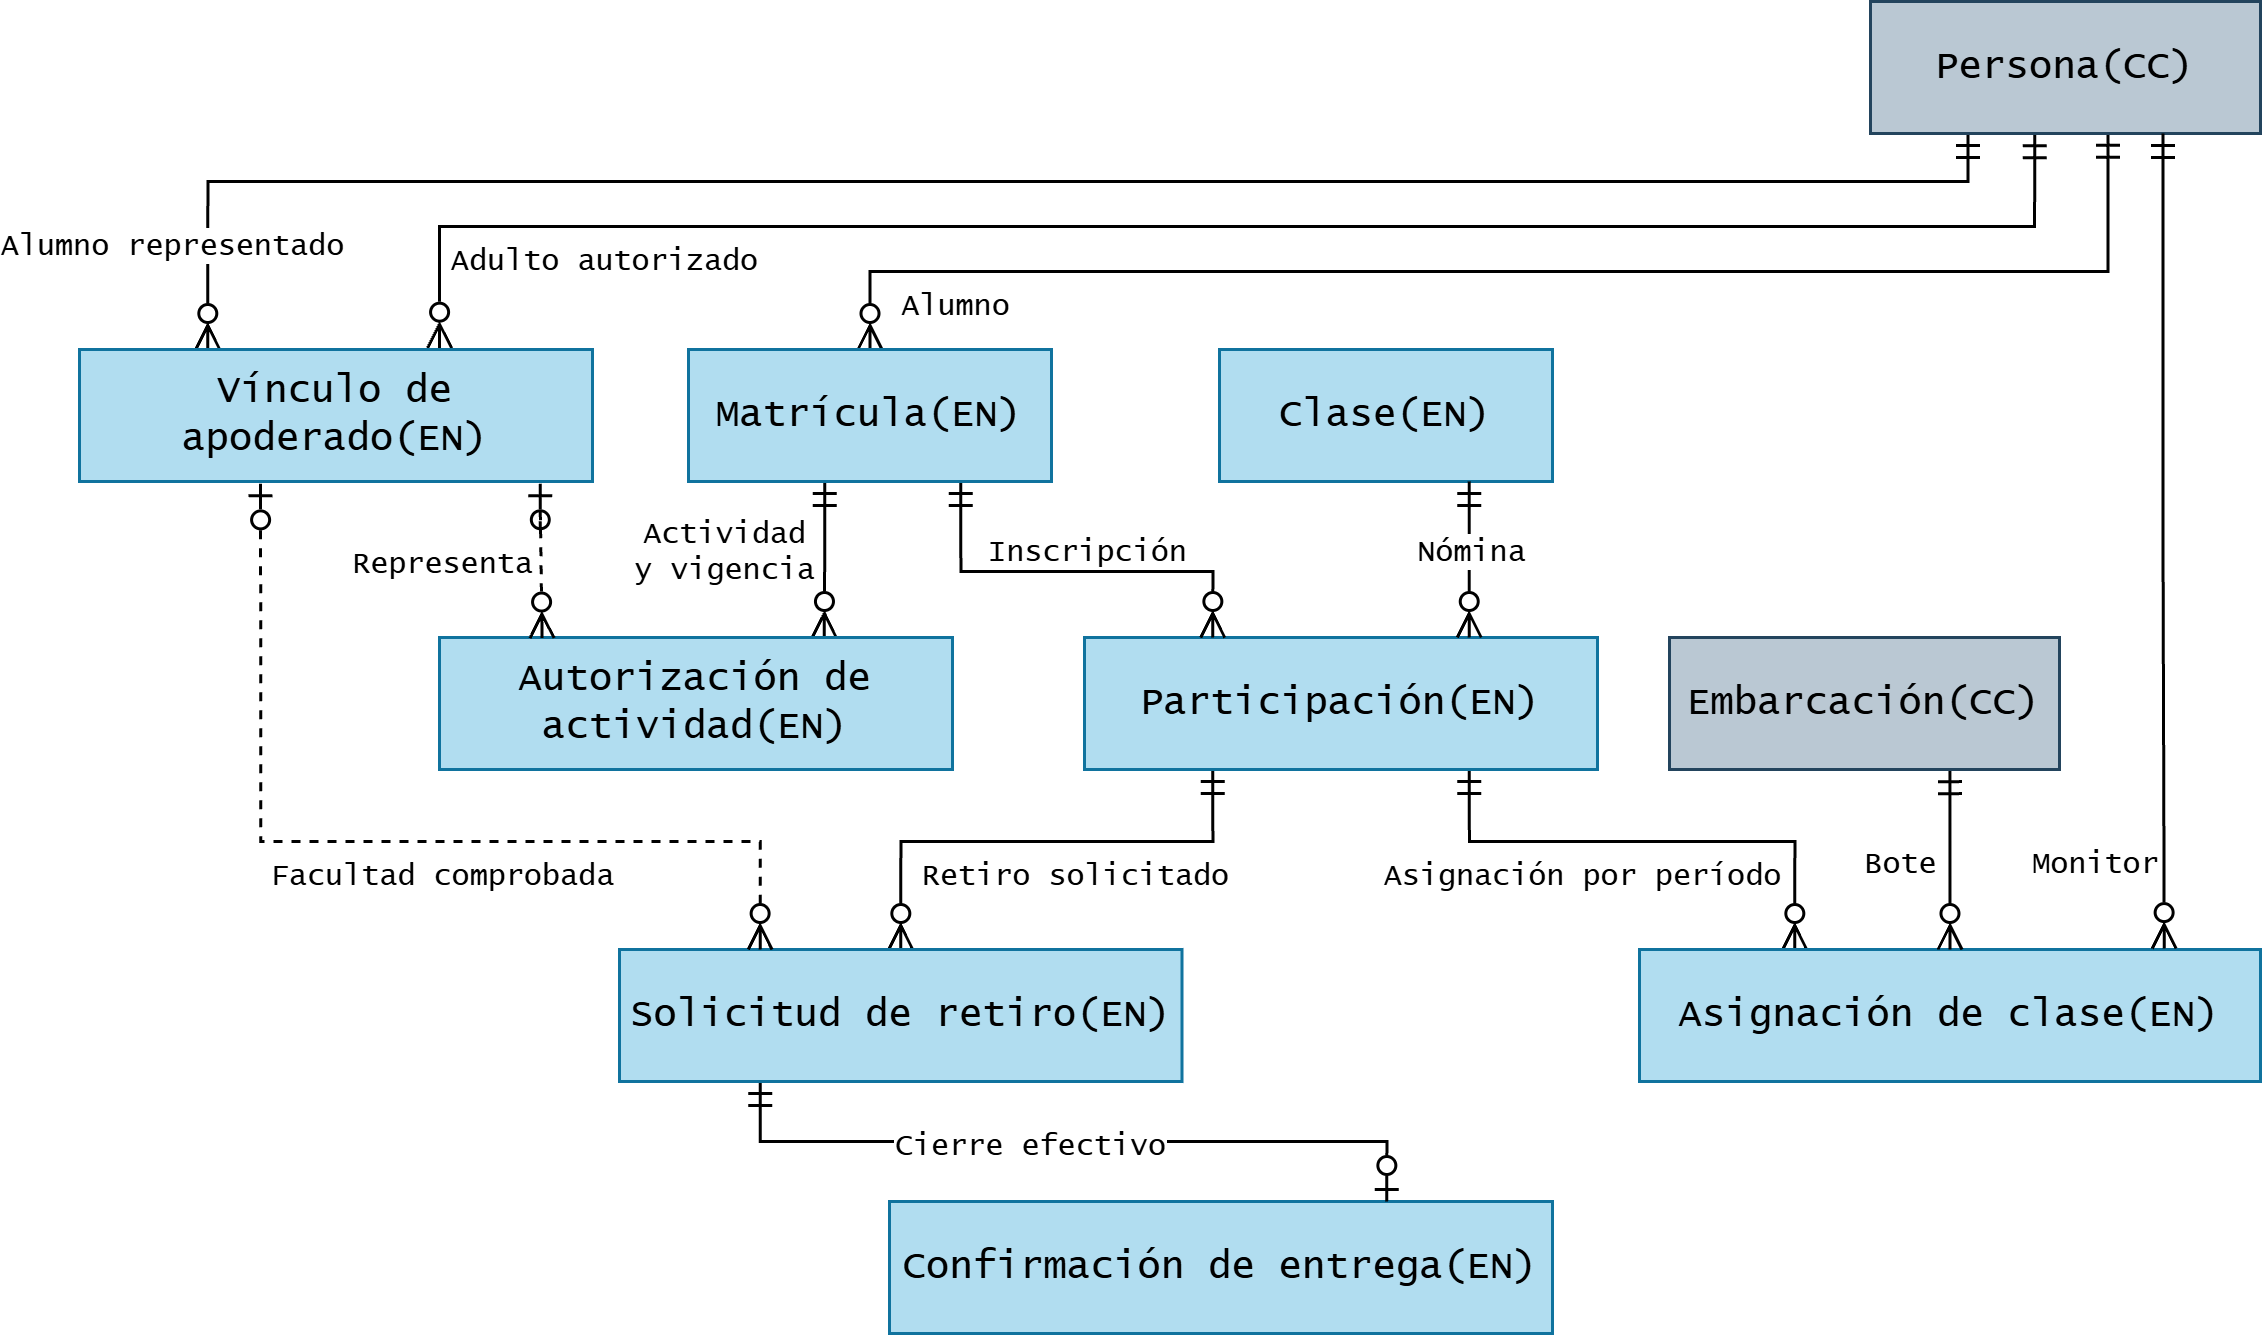
\includegraphics[width=1 \linewidth ]{figuras/F5_4.png}
    }
    \caption{Participación de escuela y retiros}
    \label{fig:escuela_nautica}
    \FuenteFigura{Modelo de datos de Synaptix; dominios y relaciones descritos en esta sección.}
\end{figure}

La participación distingue prevista, presente en tierra, en el agua, regreso confirmado, retirada y ausente. Antes de confirmar una salida deben existir autorización vigente, presencia comprobada y asignación válida, sin un retiro pendiente incompatible. Un cambio de bote o monitor cierra el intervalo anterior y abre otro con hora e informante; se impiden asignaciones simultáneas incompatibles. La proporción de alumnos por monitor se comprueba contra la política técnica versionada que corresponda a la actividad. Un incidente se conserva como registro adicional y no modifica por sí solo la situación efectiva del alumno.

El retiro avanza por solicitud, verificación de identidad, entrega pendiente y confirmación, o termina rechazado o cancelado. Portería verifica la identidad y la facultad de retiro, escuela comprueba la ubicación y la entrega segura. Ambas actuaciones quedan vinculadas a una confirmación única. Si el alumno está en el agua, la solicitud permanece pendiente hasta coordinar su entrega. Durante una interrupción de comunicaciones se utiliza el procedimiento operacional por radio, registrando informante, hora y resultado. La captura aislada no se presenta como confirmación compartida y la clase solo se cierra cuando todos los participantes tienen su regreso confirmado.

Un alumno puede tener varios adultos autorizados y un adulto puede representar a varios alumnos, además, ser contacto de emergencia no concede automáticamente permiso para retirar. La vista de emergencia incluye alertas y pautas autorizadas, contacto, vigencia y responsable de aprobación, mientras que la ficha completa permanece restringida. El acceso del monitor exige una asignación vigente y deja registro de sujeto, finalidad, dato consultado y resultado. Las autorizaciones de actividad, de retiro y de tratamiento de datos mantienen su significado propio (C07, caps. 10 y 15, RT-16.09; SD2, DEC-06/07/08).

Escuela náutica pertenece al Núcleo Operacional y conserva un subconjunto protegido para continuidad local, conforme a DA-05/16/19. Los eventos \texttt{ClaseIniciada}, \texttt{AlumnoRetirado} y \texttt{ClaseCerrada} comunican actuaciones confirmadas. El modelo desarrolla RF-ESC-02 a RF-ESC-14, RF-AUT-05, DEC-06/07/08/21 y RN-10 a RN-14. El control de acceso y la auditoría son comunes, mientras la decisión sobre participación y entrega permanece en este dominio.

\subsubsection{Varadero y contratistas}
Varadero y contratistas relaciona la programación de una faena con los antecedentes que permiten ejecutarla. Orden de trabajo identifica embarcación, solicitante, empresa contratista, actividades y estado. Maniobra conserva tipo, agenda, posiciones y recursos requeridos. Plan de izaje, Versión de plan y Validación de plan mantienen la preparación y revisión previa a la ejecución, de modo que sea posible conocer qué versión respaldó una maniobra específica y quién la validó.

Reserva de recurso vincula la actividad con un intervalo de uso de travelift, puesto, cuna o personal; Reprogramación conserva las modificaciones de agenda y su causa. Acreditación, Inducción y Habilitación de trabajador reúnen los documentos revisados, formación, resultado de evaluación y vigencia. Los trabajadores y empresas referencian Persona y Organización de Clientes y contratos. La Figura~\ref{fig:varadero_contratistas} muestra cómo el plan y las habilitaciones se relacionan con la ejecución y el acceso de faena.

\begin{figure}[htbp]
    \centering
    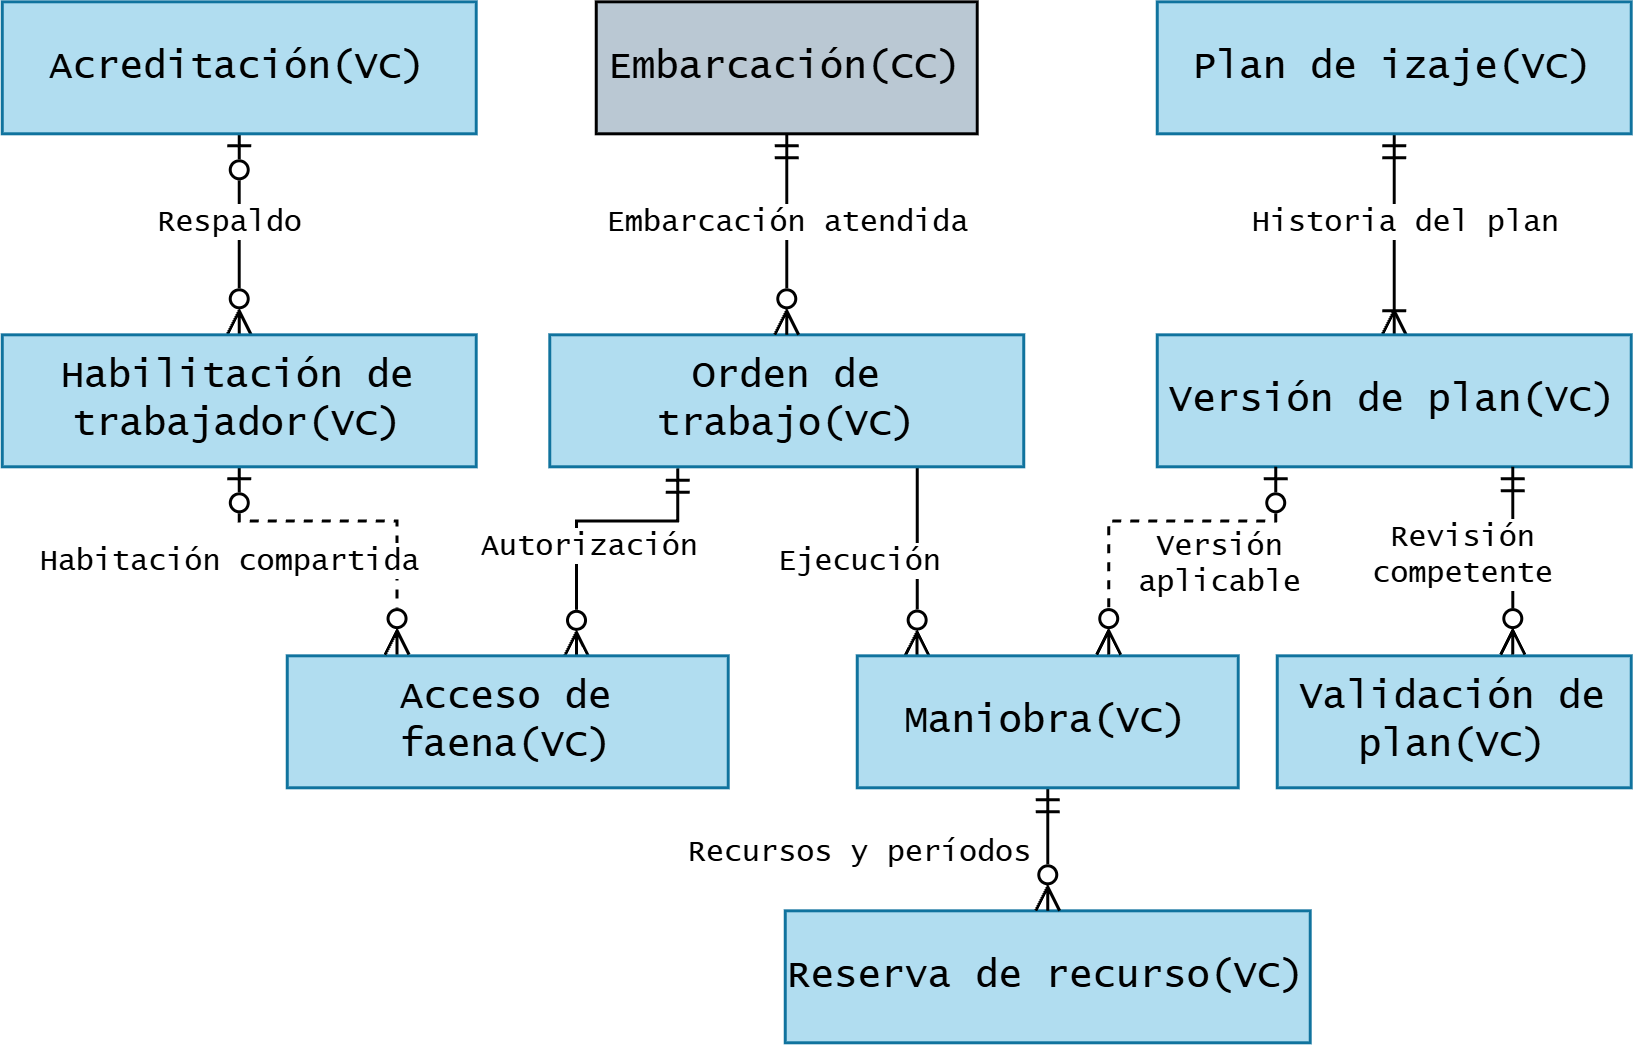
\includegraphics[width=0.8 \linewidth ]{figuras/F5_5.png}
    \caption{Faenas, plan de izaje y habilitación}
    \label{fig:varadero_contratistas}
    \FuenteFigura{Modelo de datos de Synaptix; dominios y relaciones descritos en esta sección.}
\end{figure}
\newpage
Una maniobra pasa por planificada, habilitada, en ejecución y finalizada, y puede quedar suspendida o cancelada. La planificación puede comenzar antes de disponer del plan aprobado, pero la habilitación y el inicio requieren una versión válida y aplicable a la embarcación. Las revisiones posteriores conservan la versión utilizada en la faena. Los recursos se reservan sin solapamientos incompatibles, y una suspensión por clima registra la evidencia disponible, las dependencias afectadas y la actuación del encargado. La nueva fecha se relaciona con la anterior mediante Reprogramación y conserva las comunicaciones realizadas.

Acceso de faena registra trabajador, empresa, orden, autorización, entrada, salida y resultado de los controles. Una excepción requiere motivo y aprobador competente, manteniendo los procedimientos de emergencia. El personal autorizado puede incorporar antecedentes de forma asistida, de acuerdo con la restricción de no imponer una aplicación a los contratistas. La información requerida para el izaje se registra antes de comenzar; la captura posterior documenta lo ejecutado sin exigir interacción durante la carga suspendida (SD2, DEC-12/13/15/16; C07, cap. 10).

Este dominio pertenece al Núcleo de Servicios y mantiene planes y acreditaciones vigentes disponibles en el borde según SD4, tabla 4.3. Publica \texttt{PlanAprobado}, \texttt{ManiobraFinalizada} y \texttt{AcreditaciónVencida}. El diseño se vincula con los ámbitos VAR y CTR, RF-AUT-06 y RN-15 a RN-18. La integración con control de acceso recibe la habilitación necesaria para la actuación, sin exponer el expediente completo del trabajador.

\subsubsection{Combustible}
Combustible conserva el hecho de cada expendio y los antecedentes que permiten comprobar su cantidad. Despacho identifica embarcación, operador, punto de suministro, producto, inicio, término, unidad y volumen validado. Tramo de medición relaciona el despacho con los acumulados de inicio y término, la época del contador y los cambios de instrumento. Evidencia de despacho mantiene el respaldo original y Rectificación registra las correcciones posteriores con motivo y autor.

El punto de suministro y su instrumento pertenecen a Infraestructura, mientras el dominio Combustible mantiene la operación realizada con ellos. Esta separación permite conservar la identidad física del surtidor aunque cambie el equipo de medición y evita confundir una sustitución de contador con un nuevo despacho. La Figura~\ref{fig:combustible} representa la relación entre el expendio, sus tramos y la evidencia que lo respalda.

\begin{figure}[htbp]
    \centering
    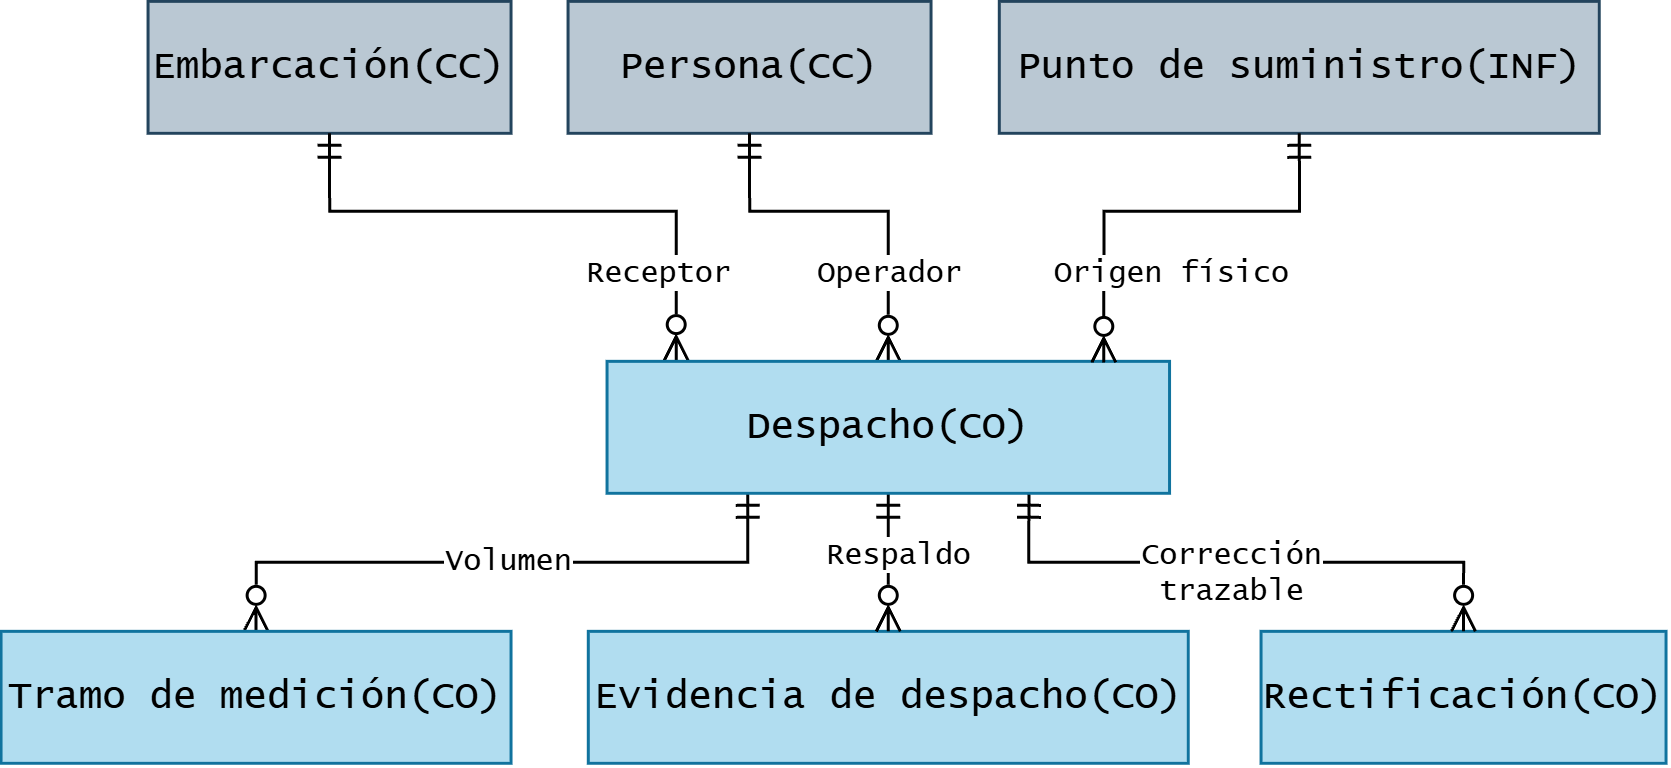
\includegraphics[width=0.8 \linewidth ]{figuras/F5_6.png}
    \caption{Despacho de combustible y evidencia original}
    \label{fig:combustible}
    \FuenteFigura{Modelo de datos de Synaptix; dominios y relaciones descritos en esta sección.}
\end{figure}
% Fuente: Elaboración del modelo a partir de SD4 tabla 4.2 y \S\,4.2; SD2/A2.1, ámbito CON.

El despacho distingue preparado, en curso, pendiente de conciliación, validado y anulado con motivo. Para cada tramo, el volumen se obtiene de lecturas compatibles del mismo instrumento y época de contador. Si existe un reinicio, cambio de escala o lectura inválida, se conserva la anomalía y se abre el tramo correspondiente, evitando interpretar una diferencia negativa como consumo válido. La suma de los tramos verificados permite consolidar el despacho; cuando la evidencia es insuficiente, permanece observado hasta resolverla.

Una corrección mantiene el dato original y agrega la rectificación autorizada. La combinación del origen instrumental, la unidad y el identificador de operación permite reconocer reenvíos del mismo expendio. El evento \texttt{CombustibleDespachado} se publica para los efectos administrativos una vez validado el hecho, y Finanzas y cobranza conserva su referencia al generar el hecho facturable. Los estados del documento contable o del pago se conocen mediante la integración externa correspondiente.

La captura se ejecuta en el Runtime Operacional de Borde y se sincroniza con el Núcleo de Servicios. El modelo desarrolla los RF del ámbito CON relativos a combustible y captura desconectada, DEC-21 y C07 RT-03.10/RT-05.10. La selección y certificación del equipo físico corresponde a SD4; este apartado define los datos que deben conservarse para identificarlo y evaluar la calidad de su evidencia.

\subsubsection{Ambiente y consumos}
Ambiente y consumos mantiene las series conciliadas de agua y energía y la trazabilidad de residuos e incidentes ambientales. Lectura original conserva medidor, secuencia, época de contador, instante, acumulado, unidad, calidad y origen. Intervalo de consumo identifica comienzo y fin, asociación temporal, cantidad y estado de conciliación. Soporte de consumo relaciona el intervalo con sus lecturas y regla de cálculo, mientras Incidencia de medición y Serie conciliada conservan observaciones, resultados y rectificaciones.

Registro de residuo identifica tipo, cantidad, unidad, recipiente, ubicación, generador declarado y registrador. Movimiento de residuo conserva los traslados; Entrega a gestor y Detalle de entrega vinculan las cantidades transferidas con sus registros de origen; Certificado mantiene la evidencia recibida. Incidente ambiental reúne derrame, respuesta, participantes y antecedentes. La Figura~\ref{fig:ambiente} muestra ambas cadenas y permite seguir el resultado hasta su origen.

\begin{figure}[htbp]
    \centering
    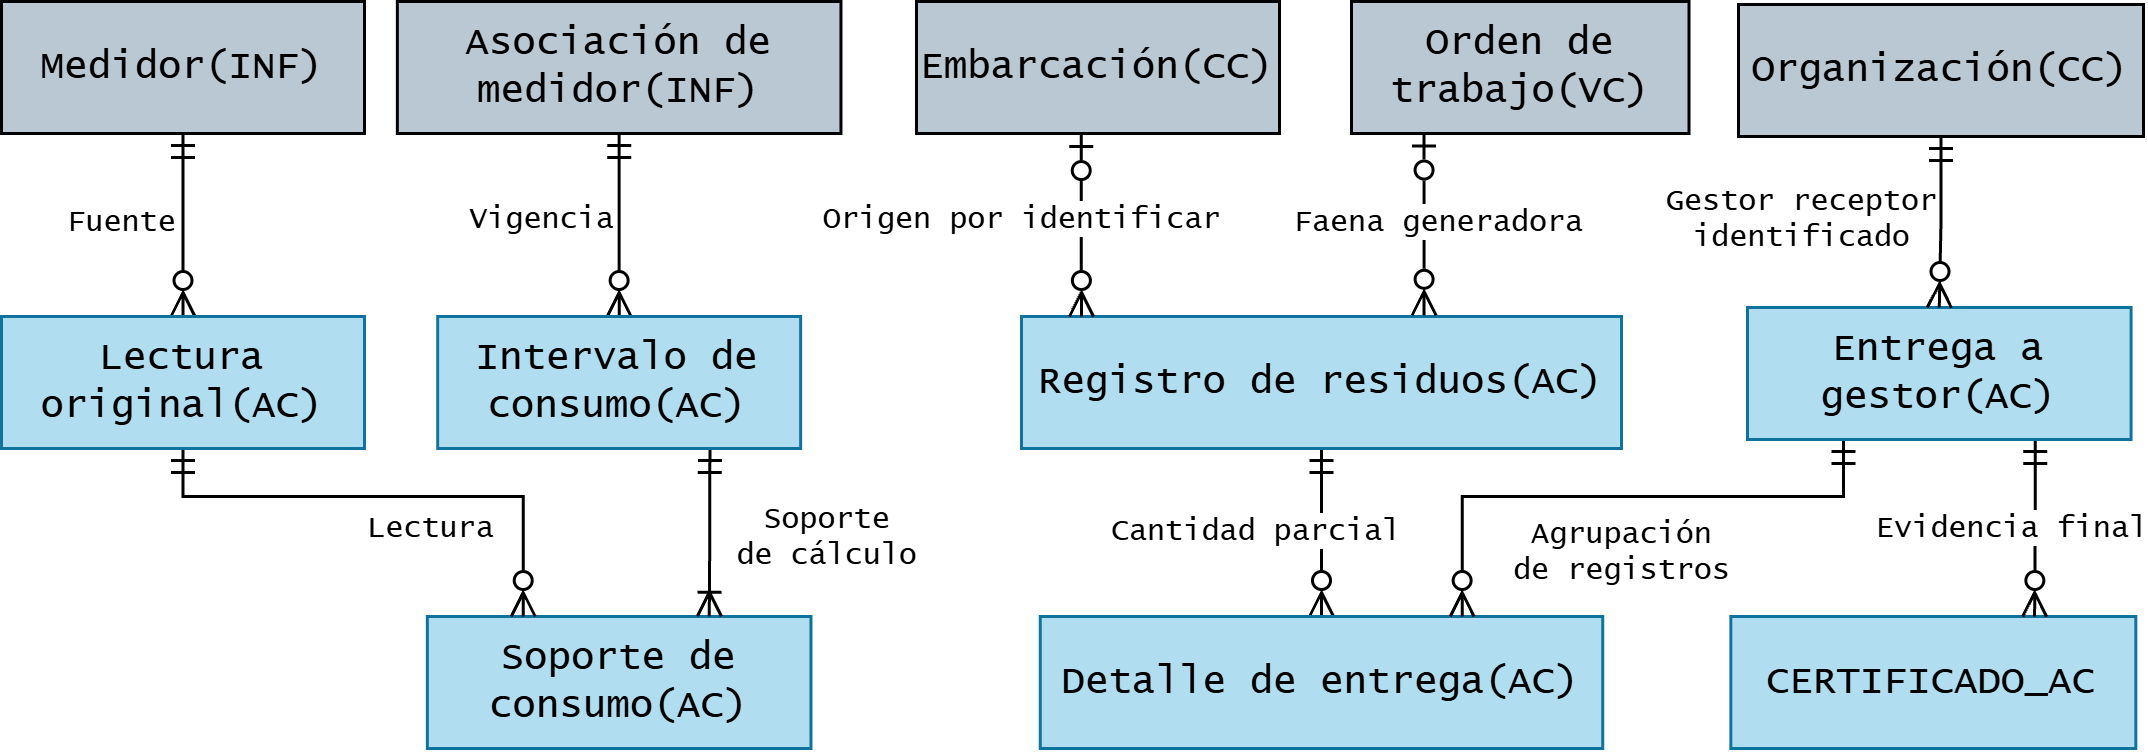
\includegraphics[width= \linewidth ]{figuras/F5_7.png}
    \caption{Consumos y trazabilidad ambiental}
    \label{fig:ambiente}
    \FuenteFigura{Modelo de datos de Synaptix; dominios y relaciones descritos en esta sección.}
\end{figure}
% Fuente: SD4 DA-09 y \S\,4.2, pp. PDF 24-25; SD2/A2.3, DEC-03/14; RN-19 a RN-21.
La Figura~\ref{fig:ambiente} muestra dos cadenas de trazabilidad. En consumos, Soporte de consumo relaciona el resultado del intervalo con las lecturas originales utilizadas para calcularlo, la asociación temporal del medidor permite reconocer a qué servicio y amarra correspondían esas lecturas. En residuos, la embarcación o la orden de trabajo se vincula con el Registro de residuo que documenta su generación o recepción. Entrega a gestor agrupa cantidades mediante Detalle de entrega, de modo que una misma entrega puede contener residuos procedentes de distintos registros y faenas.

El gestor receptor se identifica mediante Organización, cuya identidad mantiene Clientes y contratos. Como complemento de diseño, la entrega conserva la evidencia aplicable de su autorización y la comprobación de su vigencia; identificar al receptor no demuestra por sí solo que esté autorizado. El certificado recibido se vincula con la entrega efectiva y no sustituye automáticamente ese antecedente previo. Cuando no se conoce el origen del residuo, se mantiene la discrepancia y la evidencia disponible. La embarcación o faena de origen se identifica a partir de registros verificados.

Se mantiene el esquema de SD4 DA-09: un punto de agua y otro de energía por amarra, muestreo local por minuto y publicación de acumulados cada quince minutos. La asociación medidor--amarra pertenece a Infraestructura y tiene vigencia temporal. Cuando un intervalo cruza una sustitución, un cambio de asociación o de ocupante, se separa utilizando la evidencia disponible. Si falta una lectura de corte, se conserva la incertidumbre y se impide atribuir automáticamente el consumo completo al nuevo ocupante. La lectura original permanece inalterada y las correcciones producen una versión nueva del resultado conciliado.

El consumo distingue recibido, observado, conciliado y rectificado. Una lectura ausente no equivale a consumo cero; una estimación conserva método, autor y condición de uso. Solo el resultado validado, con unidad, período y asociación verificables, se publica como \texttt{MediciónConsolidada}. La serie puede respaldar tanto indicadores ambientales como hechos facturables, mientras la autorización comercial para trasladar su costo se mantiene en la regla contractual correspondiente. La adquisición por minuto y la publicación cada quince minutos son decisiones de diseño; C07 RT-05.29 exige actualización del consumo al menos horaria.

En residuos, el origen desconocido se registra como discrepancia y mantiene su investigación abierta. El modelo permite dividir una recepción en entregas parciales y agrupar varios registros en una entrega al gestor, controlando cantidades comparables y disponibilidad. La evidencia del retiro físico se conserva aunque subsista una discrepancia de origen; el cierre conciliado requiere resolverla o documentar formalmente su tratamiento. Los certificados se vinculan con la entrega efectiva, y los indicadores mantienen período, versión de regla y referencias a los registros que los sustentan.

El dominio pertenece al Núcleo de Servicios, con captura local y servicio especializado de telemetría. Publica \texttt{MediciónConsolidada}, \texttt{ResiduoRecibido} y \texttt{ResiduoEntregado}. Su trazabilidad comprende los ámbitos AMB y CON, DEC-03/14, RN-19 a RN-21 y C07 RT-05.10/29. La propiedad de la serie conciliada permanece en Ambiente y consumos, mientras Infraestructura conserva la del medidor y Finanzas y cobranza la del hecho facturable.


\subsubsection{Finanzas y cobranza}
Finanzas y cobranza relaciona los servicios prestados con su procesamiento contable y mantiene los antecedentes de las actuaciones de cobranza y custodia. Hecho facturable y Detalle de hecho identifican el origen, concepto, cantidad, unidad, período, responsable de pago, moneda y referencia a la tarifa aplicable. Lote de envío e Inclusión en lote registran cómo se remiten los hechos; Respuesta contable conserva la aceptación, observación o rechazo emitidos por el sistema externo.

Cuenta externa, Movimiento contable importado y Saldo informado mantienen referencias y versiones cuya autoridad corresponde al sistema contable. Gestión de cobranza registra comunicaciones y actuaciones; Decisión de medida conserva su propuesta, autorización y ejecución; Expediente de custodia y Antecedente de expediente reúnen la evidencia asociada al bien. La Figura~\ref{fig:finanzas} permite seguir el servicio, su respuesta externa y la documentación de custodia.

\begin{figure}[htbp]
    \centering
    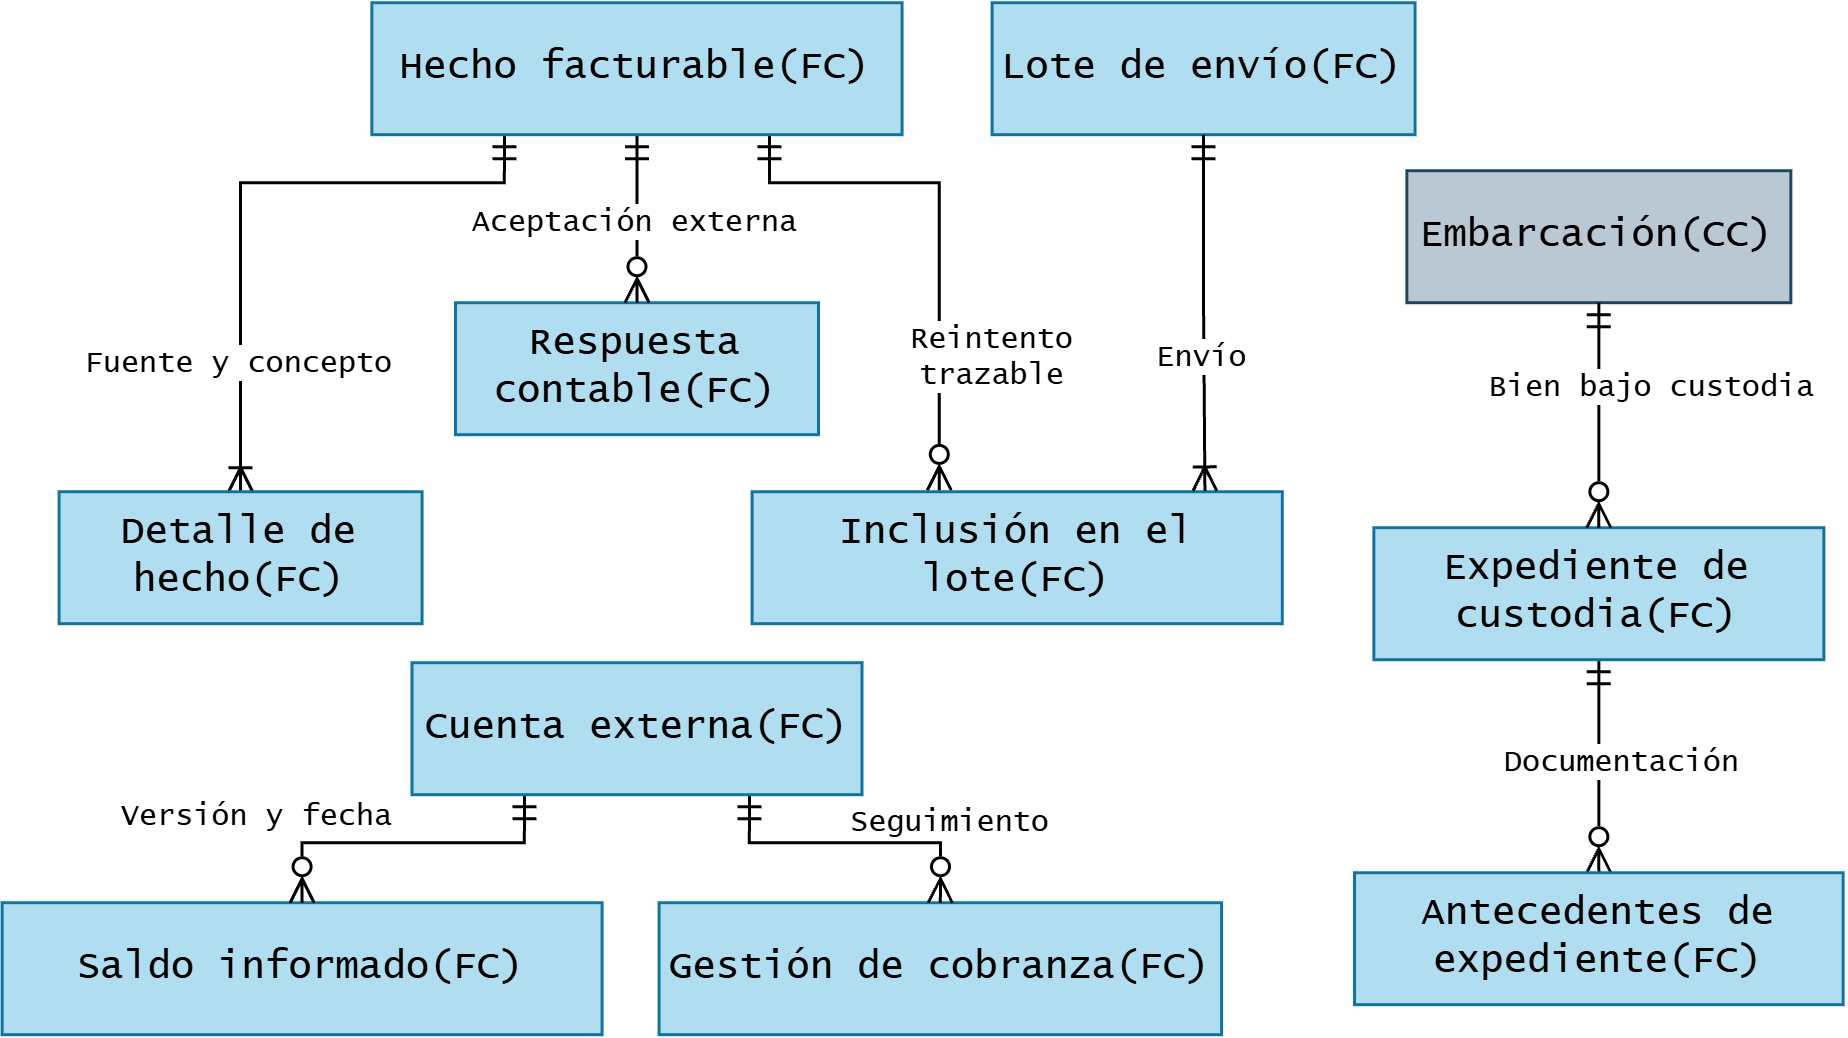
\includegraphics[width=0.86 \linewidth ]{figuras/F5_8.png}
    \caption{Hechos facturables, conciliación y custodia}
    \label{fig:finanzas}
    \FuenteFigura{Modelo de datos de Synaptix; dominios y relaciones descritos en esta sección.}
\end{figure}
%SD3 \S\,3.4.2 y SD4 \S\,4.1, autoridad contable externa; SD2/A2.3, DEC-17/18.

La clave de negocio formada por origen, versión y concepto impide duplicar un cargo por reenvío del mismo evento. El hecho pasa por preparado, observado, validado, enviado, aceptado o rechazado por contabilidad y rectificado. La aceptación registra el resultado del procesamiento externo; el pago requiere su confirmación y conciliación propias. Cuando el sistema contable agrupa o divide documentos, se conservan asociaciones identificadas en lugar de asumir una correspondencia de un documento por hecho.

Saldo informado conserva el instante al que corresponde el dato y el momento de recepción. La vista identifica una copia desactualizada y consulta la interfaz autorizada para obtener el estado vigente. El diseño mantiene el requerimiento de actualización en tiempo real de C07 RT-05.29; su comprobación depende de verificar el mecanismo disponible en contabilidad. El intercambio periódico de archivos puede apoyar una contingencia, pero no demuestra por sí solo esa oportunidad.

Las medidas de cobranza requieren una decisión competente registrada y no se activan como restricción física por el solo tramo de deuda. El expediente conserva folio, documento, versión, origen, integridad, incorporación y responsable. Para las catorce embarcaciones abandonadas se mantiene la totalidad de los antecedentes exigidos, con un índice que permita identificar documentos faltantes y su tratamiento. La exportación conserva esas relaciones y evidencia de integridad, sin reemplazar antecedentes que aún no existan (C07, cap. 10 y RT-05.15; SD2, DEC-17/18).

El dominio pertenece al Núcleo Administrativo y utiliza el adaptador contable definido en SD4. Publica \texttt{HechoFacturableGenerado} y \texttt{SaldoActualizado}, con trazabilidad al ámbito FAC, RF-AUT-03, hechos de CON/VAR/AMA y DEC-02/11/17/18. La información local pendiente corresponde a servicios o actuaciones registrados, mientras la autoridad sobre documentos tributarios, pagos y saldos permanece en el sistema externo.


\subsubsection{Infraestructura}
Infraestructura identifica los bienes físicos que utiliza el puerto y conserva su configuración e historial. Activo proporciona la identidad común y Ubicación describe su emplazamiento. Amarra agrega dimensiones y condiciones de uso; Boya, identificación y posición; Tren de fondeo y Componente de fondeo, la composición del sistema; y Medidor, servicio, unidad, número de serie y época de contador. Los puestos de invernada, cunas y equipos de varadero se registran como tipos de activo y se utilizan desde los dominios que administran sus operaciones.

Instalación de componente conserva dónde estuvo instalado cada elemento y durante qué intervalo. Asociación de medidor identifica la amarra, el servicio y la vigencia de la medición. Inspección, Hallazgo y Actuación sobre activo separan lo observado, su evaluación y la respuesta ejecutada. La Figura~\ref{fig:infraestructura} relaciona estos antecedentes y permite reconstruir la condición de un activo en un momento determinado.

\begin{figure}[htbp]
    \centering
    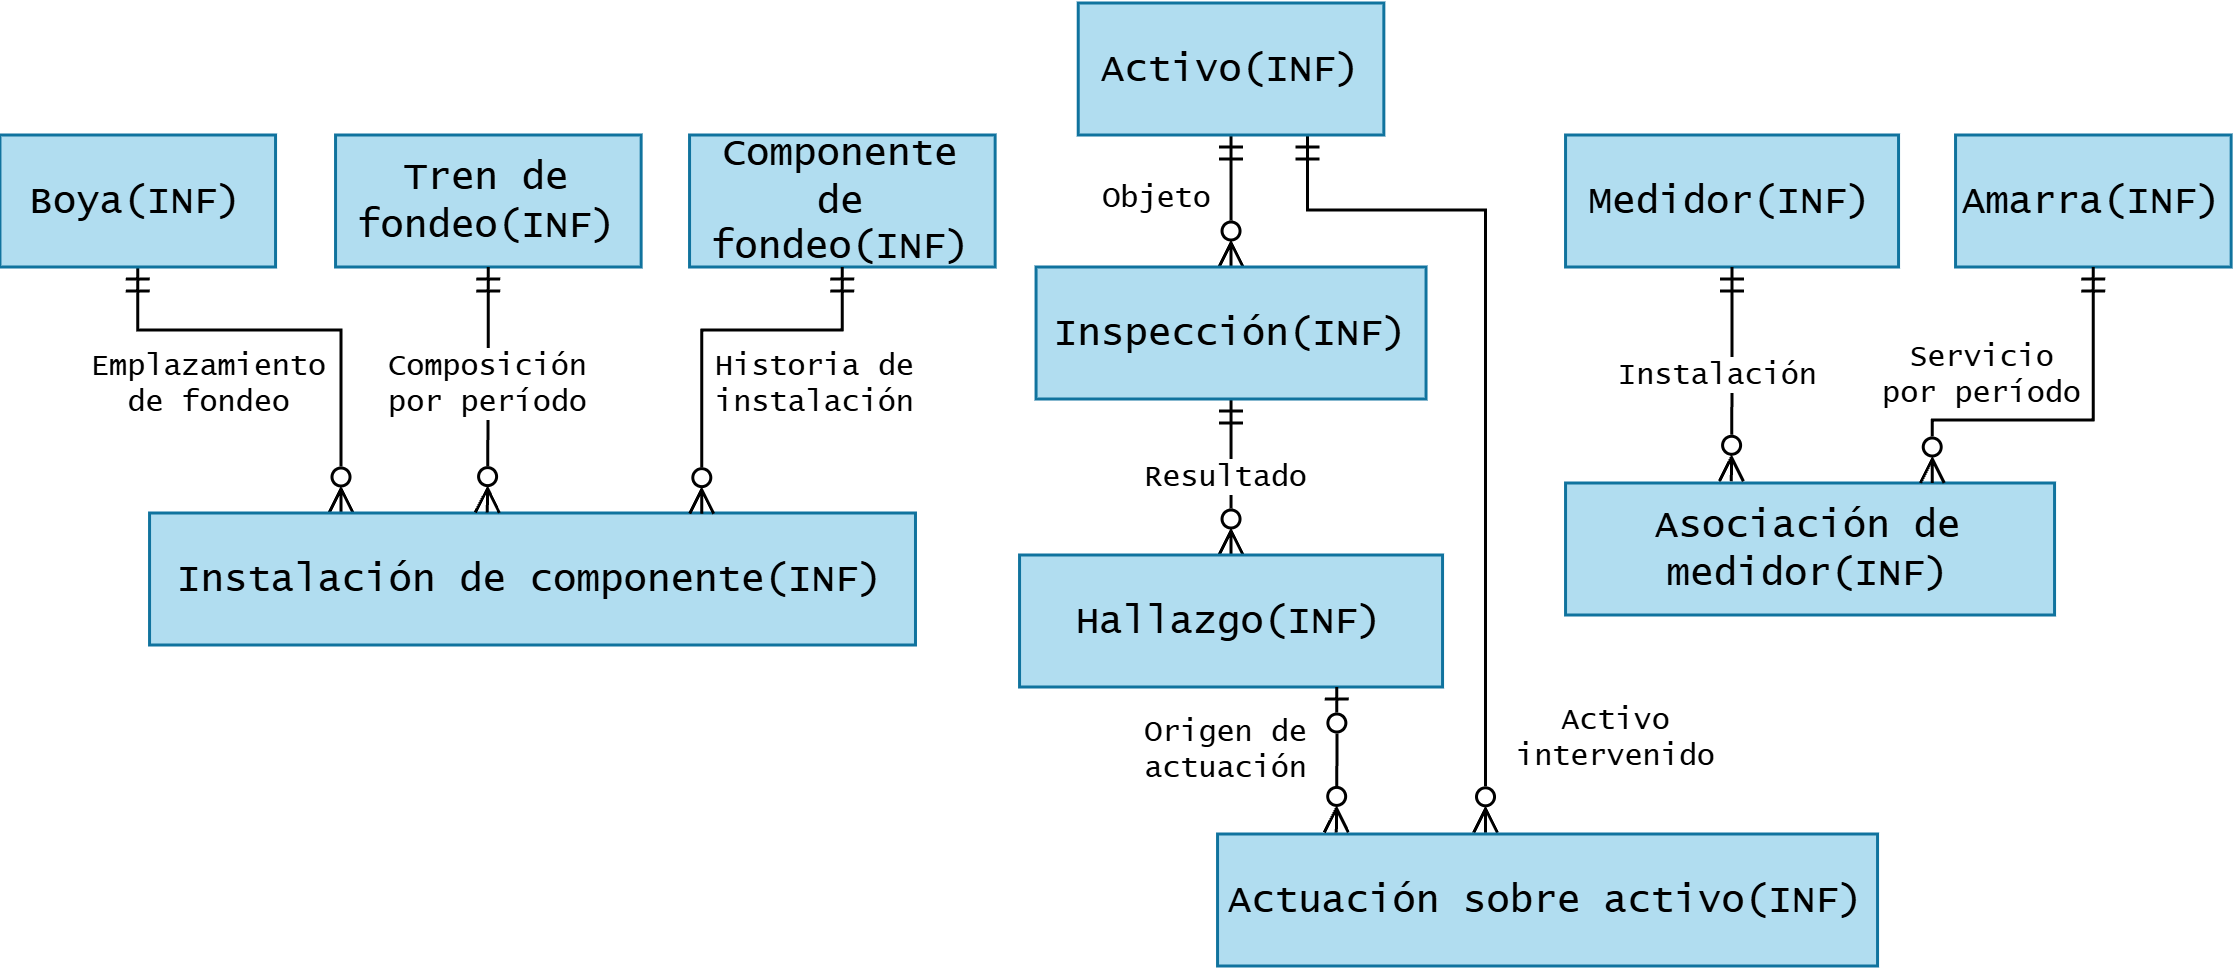
\includegraphics[width= \linewidth ]{figuras/F5_9.png}
    \caption{Activos, asociaciones de medición e inspecciones}
    \label{fig:infraestructura}
    \FuenteFigura{Modelo de datos de Synaptix; dominios y relaciones descritos en esta sección.}
\end{figure}
% Fuente: Elaboración del modelo sobre SD4 tabla 4.2 y \S\,4.2; SD2/A2.3, DEC-03/19/20.

La Figura~\ref{fig:infraestructura} separa la identidad común de Activo de las entidades que describen cada bien y su configuración. Asociación de medidor vincula un Medidor con una Amarra, un servicio y un intervalo de vigencia. Por eso, su recuadro de origen corresponde a Medidor y no a un activo de tipo indeterminado. Amarra, Boya, Medidor, Tren de fondeo y Componente de fondeo conservan su identidad de activo, que permite relacionar inspecciones y actuaciones con el mismo bien a lo largo del tiempo.

Instalación de componente conserva el componente, el tren de fondeo, la boya de emplazamiento y el período al que corresponde esa configuración. Sus referencias deben ser coherentes y no pueden permitir que un mismo componente quede como instalado simultáneamente en dos trenes. La actuación se relaciona directamente con el activo intervenido, el hallazgo previo es opcional porque también puede originarse en mantenimiento preventivo. Las cardinalidades muestran el historial y se complementan con las restricciones temporales y de compatibilidad descritas en el dominio.

Un componente no puede figurar instalado simultáneamente en dos trenes de fondeo, y un medidor no puede mantener asociaciones primarias incompatibles durante un mismo intervalo. La sustitución cierra la asociación anterior y registra la lectura de corte que respalda la nueva. Cuando existe medición de contraste, se identifica expresamente esa función para evitar sumarla como consumo adicional. Las asociaciones históricas permanecen disponibles después del retiro del equipo.

La inspección registra método, autor competente, fecha, condición, evidencia y recomendación. Una actuación conserva su activo de destino, orden y ejecución, aunque provenga de mantenimiento preventivo y no de un hallazgo previo. La periodicidad y los disparadores se vinculan con la versión del programa técnico aplicable. La vida útil del componente y los cinco años adicionales de conservación de sus inspecciones se interpretan conforme a C07 RT-05.10, manteniendo la historia tras su retiro.

La posición de la boya es parte del inventario; su ocupante y la vigencia de la observación pertenecen a Operación marítima. El dispositivo de inspección registra los datos durante el trabajo sin cobertura y conserva separadas la hora de origen y la de sincronización, conforme a la autonomía de ocho horas del caso. Este dominio pertenece al Núcleo Operacional y publica \texttt{ActivoInspeccionado}, \texttt{MedidorAsociado} y \texttt{CondiciónReportada}. Su trazabilidad comprende BOY, AMA y CON, DEC-03/19/20/21 y DA-19. Registrar el mantenimiento conserva sus resultados sin incorporar por ello su ejecución física al alcance del software.

\subsubsection{Auditoría y seguridad}
Auditoría y seguridad mantiene las evidencias que permiten comprobar quién accedió a la información y con qué autorización. Identidad de acceso relaciona el identificador del proveedor de identidad con Persona. Asignación de rol, Política versionada y Permiso operacional offline establecen funciones, alcance y vigencia. La autorización considera además la relación efectiva con el dato, como alumno a cargo, embarcación representada o expediente habilitado.

Consentimiento y Evento de consentimiento conservan otorgamiento, cambios, revocación y vencimiento. Evento de auditoría y Decisión sensible registran actuaciones y fundamentos. Documento y Versión documental proporcionan los metadatos de custodia: ubicación, formato, versión, integridad, sensibilidad y conservación; el dominio que origina el contenido conserva su responsabilidad de negocio. La Figura~\ref{fig:auditoria} presenta las relaciones entre identidad, permisos y evidencia documental.

\begin{figure}[htbp]
    \centering
    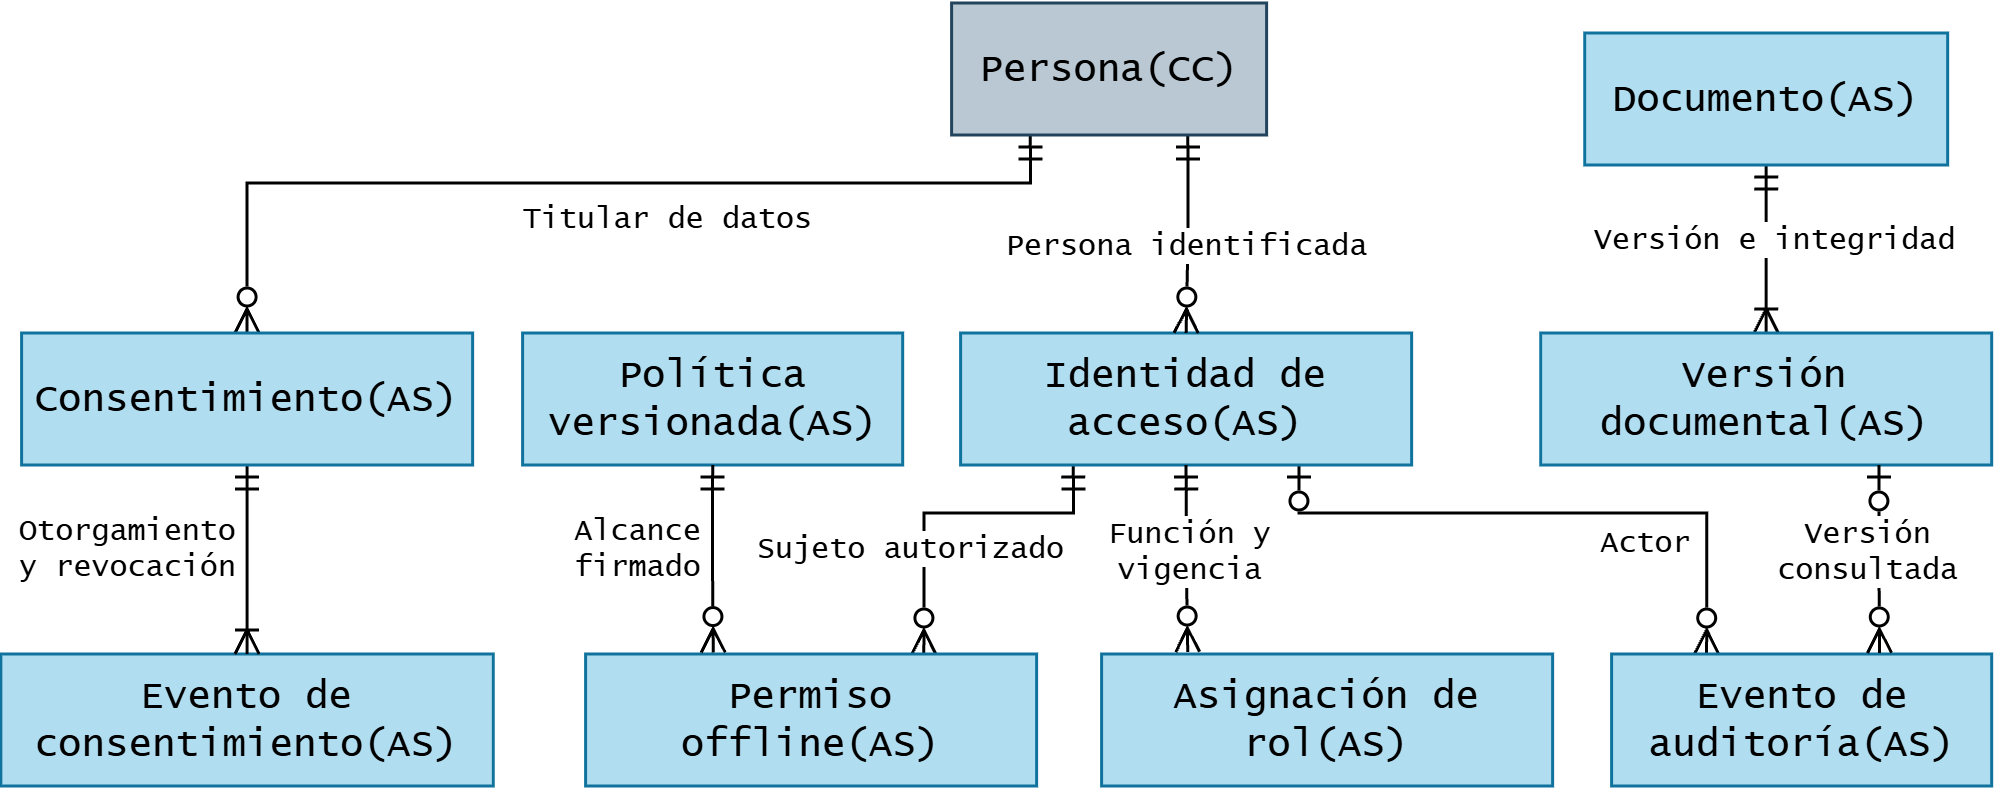
\includegraphics[width=0.9 \linewidth ]{figuras/F5_10.png}
    \caption{Identidad, consentimiento y evidencia de acceso}
    \label{fig:auditoria}
    \FuenteFigura{Modelo de datos de Synaptix; dominios y relaciones descritos en esta sección.}
\end{figure}
% Fuente: SD4 DA-16 y \S\,4.1; BT RT-05.03/08; C07 RT-16.09.

El consentimiento identifica titular, otorgante, representación cuando corresponda, finalidad, alcance, versión de la información aceptada y vigencia. Su revocación impide nuevos usos que dependan de esa autorización y conserva evidencia del acto realizado. Los antecedentes sujetos a otra obligación de conservación mantienen esa condición registrada. La autorización para participar en una clase, la facultad para retirar a un alumno y el consentimiento sobre tratamiento de datos permanecen como objetos distintos, aunque puedan compartir un documento de respaldo.

Cada evento de auditoría conserva actor humano o técnico, informante cuando sea diferente, acción, dominio, entidad, instante, dispositivo, finalidad, resultado y correlación. Los valores anteriores y posteriores se registran directamente o mediante una referencia protegida que permita reconstruirlos durante su retención. Los datos sensibles se mantienen cifrados y restringidos; los registros técnicos generales evitan reproducirlos. Las consultas a salud, datos de menores, posición compartida y antecedentes de deuda quedan auditadas aun cuando no modifiquen información (BT RT-05.03/08; C07 RT-11.10 y RT-16.09).

El permiso offline conserva sujeto, dispositivo, funciones autorizadas, política, emisión, expiración, emisor y revocación conocida. Su vigencia se rige por DA-16 y limita las acciones a las funciones operacionales permitidas. Los cambios de parámetros conservan autor y aprobador diferenciados, versión, motivo y fecha efectiva cuando su impacto lo requiere. La modalidad de firma se vincula con el tipo de acto, de modo que el sistema preserve tanto su integridad técnica como la evidencia de la autorización exigida.

Auditoría y seguridad se ejecuta como proceso especializado y mantiene controles en cada dominio, conforme a DA-08/16/19. Publica \texttt{ConsentimientoModificado} y \texttt{AccesoSensibleRegistrado}. Desarrolla RF-ADM-03/05/09 y RF-ADM-11 a RF-ADM-19, RF-ESC-11/12 y DEC-08/17/22. La seguridad verifica el acceso y conserva su evidencia; la validez de la actuación solicitada se resuelve mediante las reglas del dominio de negocio correspondiente.

\medskip
\noindent\textbf{Servicios compartidos, notificaciones y cierre del modelo}

El servicio de notificaciones relaciona un hecho de negocio con sus destinatarios y con el resultado de los contactos. Aviso conserva dominio, evento causal, contenido versionado, prioridad y autorización. Destinatario de aviso identifica persona, contacto y versión utilizados; Intento de entrega registra canal, proveedor, identificador externo, inicio y resultado. Acuse distingue aceptación del proveedor, entrega técnica, lectura y confirmación humana, mientras Tarea de escalamiento conserva las actuaciones requeridas cuando falta respuesta. La Figura~\ref{fig:notificaciones} muestra esta cadena como servicio compartido de los dominios.

\begin{figure}[htbp]
    \centering
    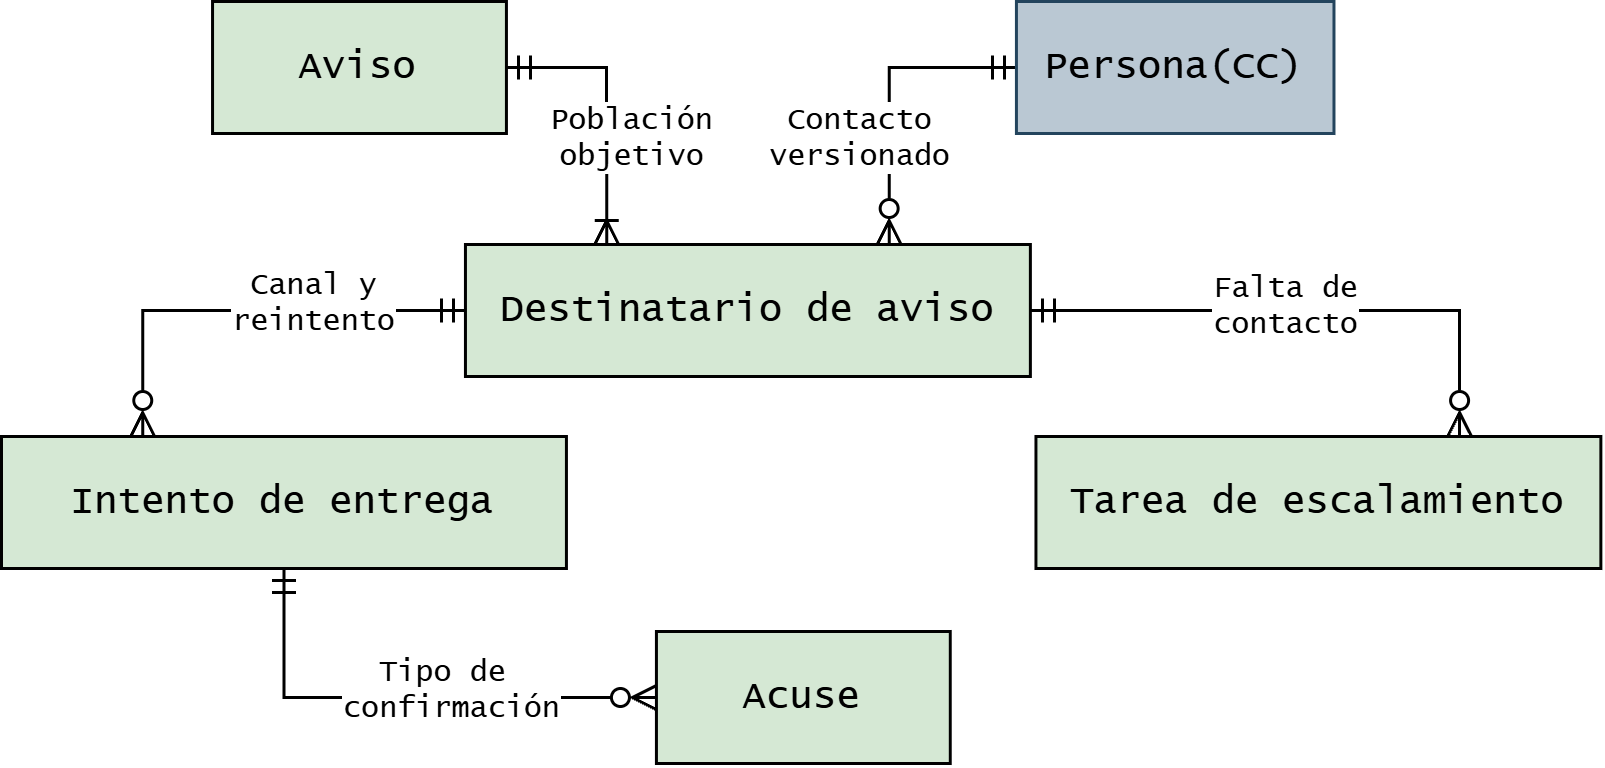
\includegraphics[width=0.75 \linewidth ]{figuras/F5_11.png}
    \caption{Notificaciones como servicio compartido}
    \label{fig:notificaciones}
    \FuenteFigura{Modelo de datos de Synaptix; dominios y relaciones descritos en esta sección.}
\end{figure}
% Fuente: SD4 \S\,4.1, servicio de notificaciones; SD2/A2.1, ALE, y A2.5, RN-06.

La campaña de emergencia conserva la población destinataria y los intentos por los canales exigidos. El tiempo hasta el último envío se mide separadamente del seguimiento de quienes no han acusado recibo. Cada tarea de llamada mantiene responsable, intentos, resultado y siguiente actuación; el silencio se conserva como falta de confirmación. La regla de escalamiento debe permitir cumplir los diez minutos máximos de envío a los 296 armadores y el seguimiento establecido por C07 RT-09.01 y RT-16.21. El servicio desarrolla el ámbito ALE y RN-06, sin convertirse en un décimo dominio canónico.

Los formularios del portal y los dispositivos utilizan estas mismas entidades y conservan el identificador de cada solicitud durante los reintentos. Su estado distingue captura, aceptación por la autoridad de negocio y confirmación de un tercero. Las copias de consulta mantienen procedencia y versión; las discrepancias conservan los antecedentes y la resolución. Así, la trazabilidad permite recorrer desde una ocupación hasta su evidencia, desde un retiro hasta la entrega confirmada y desde un cargo propuesto hasta la prestación que lo originó. 

\newpage
La Tabla~\ref{tab:sd5_invariantes_modelo} resume las condiciones que deben conservarse al implementar y verificar el modelo.

\begingroup
\setlength{\tabcolsep}{3pt}
\begin{longtable}{@{}L{.20\textwidth}L{.45\textwidth}L{\dimexpr.35\textwidth-12pt\relax}@{}}
\caption{Invariantes esenciales del modelo}\label{tab:sd5_invariantes_modelo}\\
\hline
\EncabezadoTabla{Ámbito} & \EncabezadoTabla{Condición que debe conservarse} & \EncabezadoTabla{Evidencia de control} \\ \hline
\endfirsthead
\hline
\EncabezadoTabla{Ámbito} & \EncabezadoTabla{Condición que debe conservarse} & \EncabezadoTabla{Evidencia de control} \\ \hline
\endhead
Identidad & Una identidad de negocio por entidad & Claves y vínculos vigentes \\ \addlinespace \hline
Amarras & Sin asignaciones simultáneas incompatibles & Autorización y períodos \\ \addlinespace \hline
Regreso & Declaración separada de confirmación & Informante, registrador y origen \\ \addlinespace \hline
Escuela & Retiro único y situación efectiva comprobada & Participación y confirmaciones \\ \addlinespace \hline
Medición & Sin consumo duplicado ni origen sobrescrito & Secuencia, época y lecturas \\ \addlinespace \hline
Residuos & Origen desconocido visible como discrepancia & Cadena de entrega y conciliación \\ \addlinespace \hline
Finanzas & Contabilidad externa como autoridad & Identificador y respuesta externa \\ \addlinespace \hline
Sincronización & Sin pérdida ni duplicación de efectos & Outbox, inbox y versión \\ \addlinespace \hline
Privacidad & Acceso mínimo con trazabilidad & Política, relación y auditoría \\ \addlinespace \hline
\end{longtable}
\FuenteTabla{BT RT-05.01 a RT-05.09 y parámetros de C07.}
\endgroup

Estas invariantes vinculan las reglas de negocio con sus evidencias de control. Las garantías de persistencia y sincronización se desarrollan en 5.2, mientras el diccionario A5.1 especifica los atributos y restricciones necesarios para aplicarlas.

%-----
\subsection{Datos maestros y diccionario}
Los datos maestros proporcionan las identidades y definiciones que permiten relacionar los servicios del puerto. Una misma persona puede participar como armador, apoderado o trabajador, y una embarcación puede intervenir en contratos, movimientos y servicios de varadero. Si cada módulo crea su propio registro sin una correspondencia controlada, una modificación puede dejar antecedentes contradictorios y dificultar la reconstrucción de la operación. Por ello, el modelo mantiene una identidad estable y representa los distintos roles mediante vínculos con alcance y vigencia definidos. Esta organización conserva los nueve dominios de SD4 y las entidades descritas en 5.1.1-5.1.2. Compartir una referencia mantiene la propiedad del dato en su dominio de origen y permite utilizarla sin crear registros incompatibles en cada servicio.

La gestión de maestros comprende la creación, verificación, actualización y conciliación de esas identidades. También establece quién puede autorizar una corrección y cómo se comunica a los demás dominios. El diccionario complementa esta responsabilidad de forma que se documenta qué significa cada entidad y atributo, bajo qué condiciones se utiliza y qué controles permiten interpretar su contenido.

\textbf{Identidad, autoridad y responsabilidades:} cada entidad conserva el identificador técnico estable definido en 5.1.2. Los números documentales, matrículas, códigos de activos e identificadores heredados se registran como identificadores de negocio o referencias externas, indicando su sistema emisor, ámbito y período de validez cuando corresponda. Un cambio de nombre, documento, armador, responsable o ubicación no origina por sí solo una nueva entidad. Esta separación permite conservar la continuidad del registro y reconocer los códigos utilizados por otros sistemas durante la migración y el intercambio de información.

Persona y Organización mantienen identidades distintas. Los vínculos de representación, armador y apoderado describen la relación que habilita una actuación y el período durante el cual resulta válida. Así, reconocer a una persona en el padrón no acredita automáticamente que pueda representar a una organización, modificar un contrato o retirar a un alumno. Cada dominio comprueba las facultades pertinentes a su servicio, utilizando la identidad compartida y la evidencia del vínculo correspondiente.

La autoridad se determina por entidad, atributo y actuación, conforme a la separación de responsabilidades de SD4, tabla 4.2 y DA-03/DA-05. Clientes y contratos mantienen las identidades de personas, organizaciones y embarcaciones, mientras Escuela náutica mantiene los vínculos de apoderado y autorizaciones propios de su actividad. La infraestructura registra los activos y las asociaciones temporales entre medidores e instalaciones. El sistema contable externo conserva la autoridad sobre documentos tributarios, pagos y saldos. Finanzas y cobranza utiliza sus referencias y proyecciones para conciliar los hechos del puerto.

La Tabla~\ref{tab:sd5_maestros_autoridad} resume las responsabilidades y los roles de validación funcional previstos para el diseño. La asignación nominal de responsables y suplentes se formaliza en la organización del proyecto, sin presumir que el cliente dispone de personal TI.

\begingroup
\setlength{\tabcolsep}{3pt}
\begin{longtable}{@{}L{.32\textwidth}L{.32\textwidth}L{\dimexpr.36\textwidth-12pt\relax}@{}}
\caption{Datos maestros, autoridad y validación funcional}\label{tab:sd5_maestros_autoridad}\\
\hline
\EncabezadoTabla{Conjunto de información} & \EncabezadoTabla{Autoridad del dato} & \EncabezadoTabla{Validación funcional prevista} \\ \hline
\endfirsthead
\hline
\EncabezadoTabla{Conjunto de información} & \EncabezadoTabla{Autoridad del dato} & \EncabezadoTabla{Validación funcional prevista} \\ \hline
\endhead
Personas y organizaciones & Clientes y contratos & Administración \\ \addlinespace \hline
Embarcaciones y vínculos de armador & Clientes y contratos & Administración y operaciones \\ \addlinespace \hline
Contratos y asignaciones contractuales & Clientes y contratos & Administración y aprobador comercial \\ \addlinespace \hline
Amarras, boyas, medidores y componentes & Infraestructura & Operaciones y mantenimiento \\ \addlinespace \hline
Vínculos de apoderado y autorizaciones & Escuela náutica & Responsable de escuela \\ \addlinespace \hline
Catálogos y reglas de servicio & Dominio que aplica la regla & Jefatura funcional, aprobación de un segundo perfil con justificación para cambios con impacto operacional \\ \addlinespace \hline
Identidades y permisos de acceso & Proveedor de identidad; Auditoría y seguridad & Perfil funcional autorizado \\ \addlinespace \hline
Documentos tributarios, pagos y saldos & Sistema contable externo & Administración; conciliación en Finanzas y cobranza \\ \addlinespace \hline
\end{longtable}
\endgroup

Clientes y contratos mantiene la identidad de una embarcación, pero la Operación marítima registra sus movimientos y la conclusión sobre su situación operacional. Infraestructura mantiene la instalación de un medidor y Ambiente y consumos interpreta las lecturas dentro del intervalo correspondiente. Del mismo modo, disponer de una copia de un saldo permite consultarlo con su fecha de actualización, pero no habilita a Finanzas y cobranza para sustituir el saldo autorizado por el sistema contable.

Los catálogos y reglas de cada servicio conservan versión, vigencia y aprobador. Todo cambio de parámetro con impacto operacional requiere validación funcional, aprobación de un segundo perfil y justificación registrada. En contratos y asignaciones contractuales se mantiene la administración de versiones en nube establecida en SD4, diferenciada de la autoridad local para las actuaciones operacionales descritas en 5.1.2.

Los consumidores acceden a estos antecedentes mediante los contratos de intercambio definidos por el propietario. Sus proyecciones conservan origen, versión y fecha de actualización para determinar si el dato disponible resulta adecuado para la actuación solicitada. Las claves externas se verifican mediante esos contratos o sus proyecciones autorizadas, no se habilitan escrituras ni consultas directas entre esquemas ajenos. 

\textbf{Alta, actualización y conciliación de identidades:} antes de crear un maestro se revisan los identificadores disponibles y las coincidencias relevantes. Un identificador verificado permite localizar una identidad existente, una coincidencia de nombre o contacto genera una revisión y requiere comprobar antecedentes adicionales, sin desencadenar una fusión automática. Cuando se localiza la entidad, el nuevo hecho se vincula con ella y las modificaciones se tramitan conforme a los permisos del dominio propietario. Cada cambio conserva su fuente, responsable, fecha y evidencia.

Durante una atención sin conexión puede ser necesario registrar una persona o embarcación que no aparece en el padrón disponible. En ese caso, se conserva una referencia provisional con identificador estable, origen y datos mínimos para identificar la actuación. Esta referencia permite mantener el hecho operacional y sus evidencias mientras se resuelve la identidad. El registro del hecho y sus evidencias se conserva aunque la identidad esté pendiente. Su carácter provisional permanece visible, es decir, no se presenta como maestro central validado ni acredita por sí solo representación, permisos o una decisión exclusiva sobre recursos compartidos.

Al recuperar la comunicación, el dominio propietario revisa los antecedentes y determina si corresponde vincular la referencia con un maestro existente, aprobar una identidad nueva o mantener la resolución pendiente. Para personas y embarcaciones, esa revisión corresponde a Clientes y contratos. Si los antecedentes son insuficientes, el registro conserva su condición pendiente y se solicita la información necesaria, manteniendo identificable la operación ya registrada. El procedimiento de transporte, reintento y recepción se desarrolla en 5.2.2, la aceptación de la identidad requiere además esta validación de negocio.

La Figura~\ref{fig:datos_maestros} presenta el recorrido desde la solicitud inicial hasta la distribución de la identidad resuelta.

Los colores del diagrama describen funciones: el gris identifica el inicio del proceso; el azul, las actividades de búsqueda, revisión, actualización e intercambio; el amarillo, las preguntas o decisiones que separan caminos; el verde, las confirmaciones y resultados aceptados; el naranjo, las situaciones provisionales o pendientes de resolución; el violeta, una regla de conservación que se aplica al proceso.


\begin{figure}[htbp]
    \centering
    \makebox[\linewidth][c]{%
        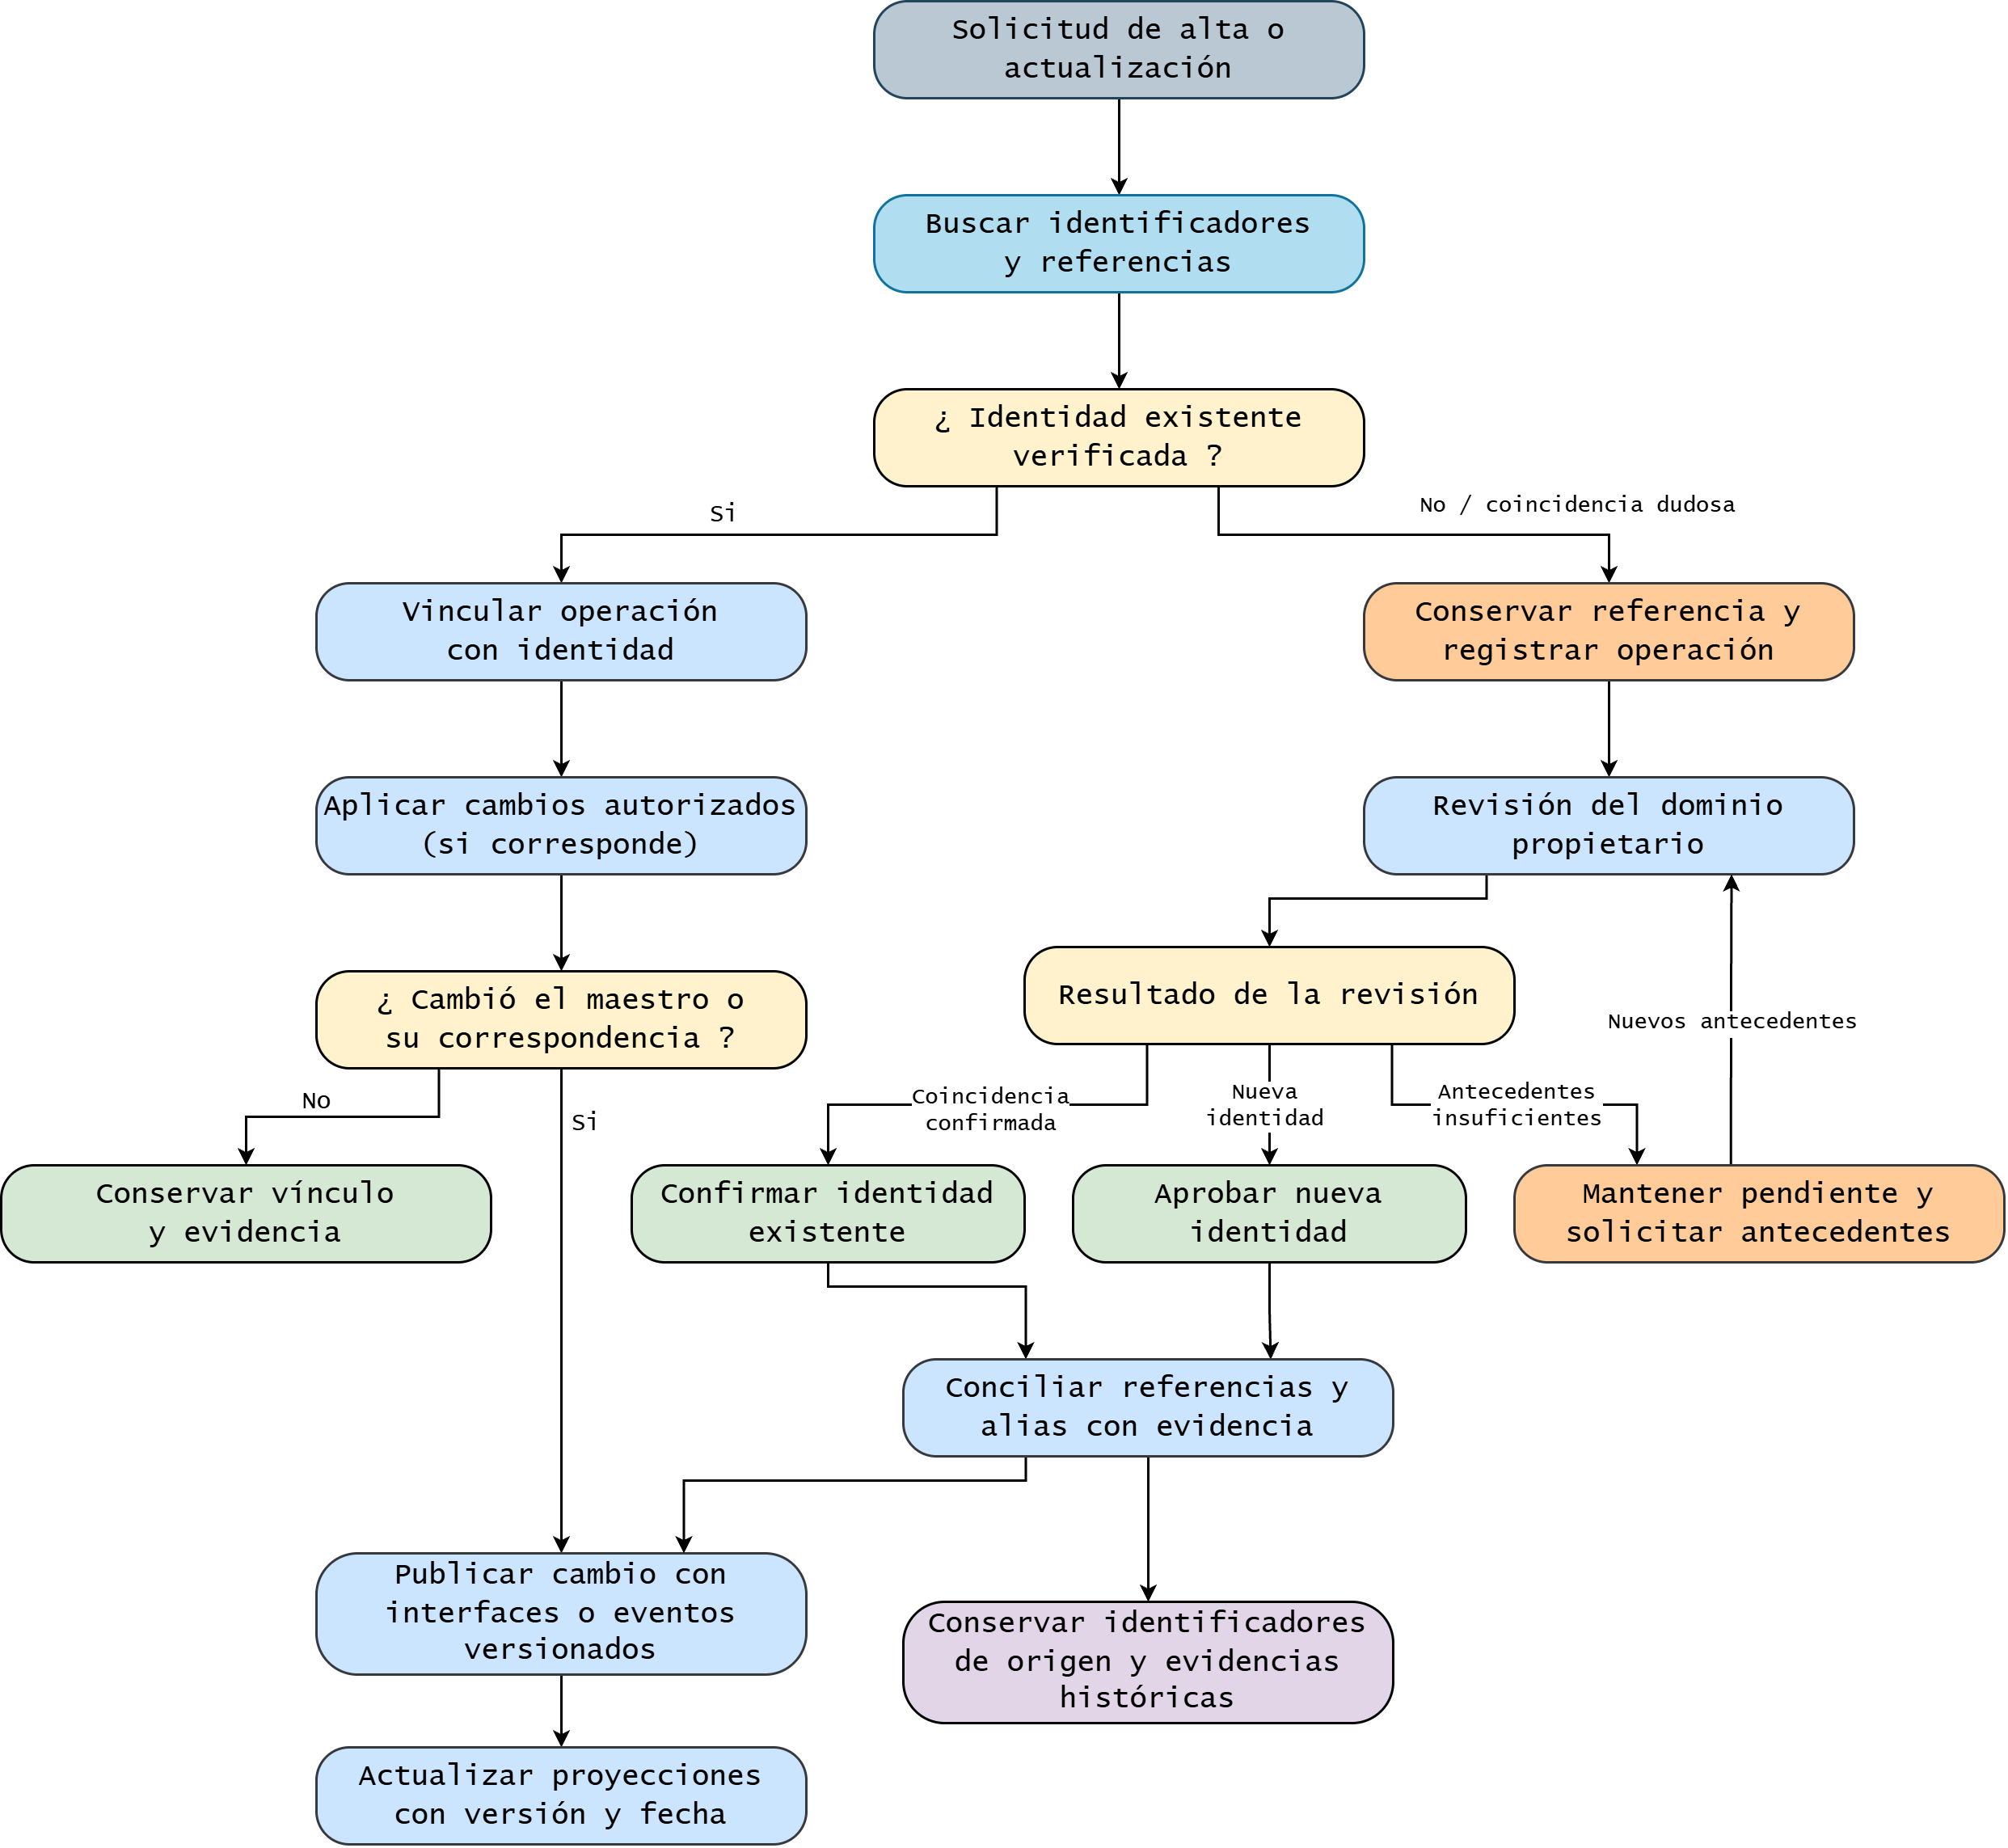
\includegraphics[width=\linewidth]{figuras/F5_12.png}
    }
    \caption{Proceso de identificación y conciliación de datos maestros}
    \label{fig:datos_maestros}
    \FuenteFigura{Flujo de conciliación de Synaptix; autoridad y correspondencias descritas en esta sección.}
\end{figure}
\newpage

La figura muestra que la confirmación de una identidad existente y la aprobación de una nueva conducen a una correspondencia explícita entre el identificador provisional, los códigos heredados o externos y la identidad canónica. Esa correspondencia permite a los consumidores actualizar sus proyecciones sin volver a decidir la identidad por cuenta propia. Cuando una identidad verificada solo requiere vincular una operación, se conserva ese vínculo. La publicación de un cambio procede cuando efectivamente se modifica el maestro o sus correspondencias.

La conciliación debe preservar la explicación histórica del registro. Una fusión requiere evidencia y autorización, conserva los identificadores anteriores como alias y registra las relaciones afectadas. El contenido firmado y el informante original de los hechos permanecen íntegros. Si una fusión resulta incorrecta, su separación posterior debe reconstruir las referencias y relaciones afectadas, registrar la corrección y comunicar el ajuste a los consumidores mediante interfaces o eventos versionados. Las proyecciones conservan la versión y la fecha de actualización para reconocer la correspondencia utilizada. Por tanto, recibir y sincronizar un registro no equivale automáticamente a aprobar su identidad(la figura representa esa diferencia entre recepción técnica y resolución funcional).

\textbf{Contenido y utilización del diccionario:} el anexo A5.1 concentra la especificación de las entidades y atributos del modelo. Cada entrada documenta nombre funcional y técnico, definición, tipo, precisión, dominio de valores, obligatoriedad, propietario y sensibilidad. El diseño incorpora además unidad cuando corresponda, condición de uso, clave o referencia, origen, regla de validación, clasificación de acceso, regla de retención y correspondencia con RF/RNF y DEC aplicables. Estos campos complementan el mínimo exigido sin trasladar al anexo la explicación de los modelos del cuerpo.

Estas definiciones permiten comprobar que formularios, interfaces, almacenamiento y migración interpretan el dato de la misma manera. Por ejemplo: \texttt{occurredAt} identifica el momento informado de ocurrencia de un hecho y \texttt{recordedAt} el momento en que se registró. La diferencia resulta necesaria cuando un dispositivo recupera la conexión después de la operación. Una medición de combustible requiere unidad y precisión decimal. Un totalizador o lectura acumulativa necesita época de contador y secuencia para reconocer reinicios. Un identificador externo requiere su sistema emisor para evitar coincidencias aparentes entre códigos de distinto origen.

El diccionario también especifica cómo se representan un valor ausente, un valor cero y una condición que no aplica. Para los estados, se documenta su significado, las transiciones permitidas, el rol autorizado y la evidencia requerida. Así se conserva la distinción entre una declaración, una solicitud y una confirmación efectiva desarrollada en 5.1.2. Las relaciones temporales indican su inicio, término y condición de vigencia, de modo que pueda reconstruirse qué vínculo era válido al ocurrir el hecho.

\textbf{Versionamiento y control de cambios:} el diccionario se registra cada version junto con los esquemas y contratos de intercambio. Un cambio de significado, unidad, sensibilidad o estado requiere revisar los consumidores, la migración, los permisos, la retención y las pruebas antes de desplegarse. Renombrar una columna no resuelve por sí solo un cambio de significado. El responsable funcional valida el significado del cambio y se comprueban sus efectos técnicos, utilizando las responsabilidades del proyecto y conservando la evidencia de aprobación correspondiente.

La revisión de integración comprueba que cada atributo persistido tenga una definición, cada entidad tenga propietario y cada referencia utilice una versión compatible y no apunte a estados eliminados. La gestión cotidiana de calidad y correcciones se desarrolla en 5.2.4, mientras que en la 5.2.5 establece protección y ciclo de vida.El anexo A5.1 reúne el detalle que permite aplicar estos controles y describir su estructura.








%---------------------------------------------
\newpage
\section{Gestión de datos}
La gestión de datos convierte el modelo en reglas de conservación, procesamiento y acceso aplicables en nube, recinto y dispositivos. Se adopta como base arquitectónica el SD4 v0.1 recibido. Las especificaciones de este apartado precisan su aplicación al dato de autoridad de escritura, resultado de cada confirmación, límites de las proyecciones y evidencia necesaria para comprobar el funcionamiento. Las precisiones nuevas son parte del diseño propuesto, no se presentan como acuerdos ya validados por el cliente.

\subsection{Persistencia y consistencia}
\label{subsec:sd5_persistencia}

El paradigma principal es relacional. Contratos, participaciones de alumnos, asignaciones, maniobras, despachos y hechos facturables requieren relaciones explícitas, estados controlados y restricciones que se evalúen al confirmar una operación. Se conserva PostgreSQL 18 como línea base para  la nube y el recinto, con migraciones versionadas y mantenimiento de versiones soportadas. La línea de versión se mantiene conforme al ciclo de soporte y a las migraciones probadas, no se heredan automáticamente las versiones distintas mencionadas en documentos anteriores.

La selección de PostgreSQL se fundamenta en su correspondencia con los controles del caso: las referencias vinculan contratos, embarcaciones y puestos. La unicidad identifica operaciones, y las restricciones de exclusión permiten expresar incompatibilidades entre intervalos. El aislamiento y los bloqueos complementan esas restricciones cuando la confirmación depende de decisiones concurrentes. Emplear el mismo motor en nube y recinto permite mantener un esquema y reglas de migración compatibles, aunque cada despliegue conserve su autoridad y sus recursos.

Los nueve dominios comparten esta selección para sus datos transaccionales. Los repositorios de documentos, las copias móviles y los conjuntos analíticos cumplen funciones complementarias, pero ninguno adquiere por ello autoridad sobre las entidades de otro dominio.

\textbf{Distribución de la persistencia:} PostgreSQL mantiene entidades, relaciones, transacciones, metadatos y bandejas de eventos. Amazon S3 conserva documentos y evidencias mediante objetos versionados referenciados desde el modelo. La aplicación Android utiliza Room sobre SQLite para el subconjunto operacional y su cola durable, Room proporciona una capa de acceso a SQLite y no sustituye el diseño de cifrado, autorización ni sincronización (Android Developers, s.\,f.). Parquet y Athena se reservan para explotación analítica. Cada medio responde a una necesidad distinta. Un objeto o un mensaje no reemplaza la transacción que acredita un hecho de negocio.

Frente a un núcleo documental o clave-valor, se prefiere el modelo relacional porque las relaciones e invariantes del caso son numerosas y estables. Un almacén de documentos simplificaría determinados contenidos variables, pero trasladaría a la aplicación controles de vínculos, vigencia y conciliación que aquí son centrales. S3 resuelve los binarios sin convertirlos en filas de gran tamaño. PostgreSQL conserva su identificación, propietario, clasificación, versión, huella de integridad y estado de verificación. No se incorpora un motor adicional de series temporales.

\textbf{Unidad transaccional y concurrencia:} La unidad de confirmación es la operación dentro de su dominio y autoridad. Dato de negocio, versión, registro de auditoría local y evento de salida se confirman en una misma transacción. Una falla previa al cierre revierte esos efectos. En el receptor, la marca de deduplicación y el efecto aplicado se confirman también conjuntamente. El envío por red ocurre fuera de esa transacción y admite reintentos.

PostgreSQL permite restricciones de unicidad, referencia y exclusión, además de distintos niveles de aislamiento. Se propone usar restricciones para invariantes declarativas y serialización o bloqueos sobre el recurso afectado cuando una decisión dependa de lecturas concurrentes. Las fallas de serialización deben provocar el reintento completo y acotado de la transacción, conservando la clave idempotente. En particular, dos solicitudes de una misma amarra no se resuelven mediante una consulta libre seguida de dos escrituras independientes. El control se realiza sobre la autoridad de asignación operacional y el intervalo solicitado.

No se extiende esa atomicidad a la nube, recinto, dispositivos incomunicados y sistemas externos. Una operación que involucra varios dominios conserva pasos y resultados explícitos como: solicitada, aceptada, rechazada o pendiente de conciliación según el proceso. La reversión de un cobro propuesto o de una reserva se expresa mediante una corrección trazable, esto no borra el despacho o la presencia física que efectivamente ocurrieron. Para evidencias binarias se emplea carga provisional, verificación de integridad y vinculación confirmada. Un archivo aún no recibido no se marca como disponible ni se elimina del origen por un acuse de sus solos metadatos.

\textbf{Consistencia y disponibilidad ante particiones:} CAP establece el límite entre consistencia fuerte de una copia lógica distribuida y respuesta a todas las solicitudes durante una partición de red. No clasifica de forma absoluta un producto ni elimina la integridad de una transacción local. En este diseño se restringen las escrituras exclusivas a la autoridad correspondiente y se mantiene la captura local de hechos, cuyas proyecciones remotas convergen al reconectar. 
La Tabla~\ref{tab:sd5_consistencia_dominios} precisa el compromiso por dominio, evitando prometer actualidad global mientras existe aislamiento.

\begingroup
\setlength{\tabcolsep}{3pt}
\begin{longtable}{@{}L{.24\textwidth}L{.20\textwidth}L{.28\textwidth}L{\dimexpr.28\textwidth-18pt\relax}@{}}
\caption{Autoridad y consistencia ante pérdida de conectividad}\label{tab:sd5_consistencia_dominios}\\
\hline
\EncabezadoTabla{Dominio} & \EncabezadoTabla{Autoridad de escritura} & \EncabezadoTabla{Confirmación exclusiva} & \EncabezadoTabla{Disponibilidad local} \\ \hline
\endfirsthead
\hline
\EncabezadoTabla{Dominio} & \EncabezadoTabla{Autoridad de escritura} & \EncabezadoTabla{Confirmación exclusiva} & \EncabezadoTabla{Disponibilidad local} \\ \hline
\endhead
Clientes y contratos & Nube & Maestros y contratos & Consulta versionada \\ \addlinespace \hline
Operación marítima & Recinto & Puesto y maniobra & Captura operacional \\ \addlinespace \hline
Escuela náutica & Recinto & Participación y entrega & Captura y coordinación \\ \addlinespace \hline
Varadero y contratistas & Según actuación & Plan y acreditación vigentes & Consulta y ejecución \\ \addlinespace \hline
Combustible & Recinto & Despacho identificado & Captura de despachos \\ \addlinespace \hline
Ambiente y consumos & Recinto & Consumo validado & Lecturas y residuos \\ \addlinespace \hline
Finanzas y cobranza & Dominio / contabilidad & Documento, pago y saldo externos & Hechos pendientes \\ \addlinespace \hline
Infraestructura & Según actuación & Maestro autorizado & Inventario e inspección \\ \addlinespace \hline
Auditoría y seguridad & Central / local & Política central vigente & Evidencia durable \\ \addlinespace \hline
\end{longtable}
% Fuente de referencia: SD4, tablas 4.2--4.3 y DA-05/DA-06/DA-16; BT RT-05.02; C07 RT-03.10.
\endgroup

La tabla distingue la disponibilidad de captura de la posibilidad de confirmar una decisión exclusiva. Clientes y contratos priorizan consistencia, es decir, sin acceso a la autoridad central, sus copias permiten consultar versiones, pero no aprobar nuevos cambios. La Operación marítima, Escuela náutica y Combustible mantienen la autoridad operacional del recinto y proyectan sus hechos hacia nube al reconectar. Un dispositivo aislado conserva hechos y solicitudes, no arbitra por sí solo un puesto o una entrega compartidos con otro equipo.

En Varadero y contratistas, la ejecución puede registrarse localmente, pero una copia antigua no acredita una aprobación nueva. La Infraestructura conserva la separación entre cambios maestros autorizados e inspecciones capturadas en terreno. Ambiente y consumos recibe lecturas y registros de residuos. Una serie pendiente de validación no produce un consumo facturable confirmado. Finanzas y cobranza conserva sus hechos y difiere los efectos que dependen de contabilidad externa. Auditoría y seguridad conserva evidencia local con permisos acotados, mientras la actualización de políticas requiere su autoridad central.

Así, la consistencia de decisiones exclusivas se protege en la autoridad correspondiente y la disponibilidad de captura se mantiene dentro de su alcance. Las proyecciones entre sitios son de convergencia eventual, Durante una partición no se promete una versión global actualizada. Esta postura se aplica por operación y dominio, sin declarar consistencia fuerte y disponibilidad total simultáneas entre copias incomunicadas.

La continuidad local no equivale a escritura simultánea de dos primarios. El mecanismo de conmutación del SD4 debe aislar al nodo anterior antes de habilitar al sustituto. Si no puede establecerse una autoridad única, se conserva la captura identificada en dispositivos, pero no se emiten decisiones exclusivas incompatibles. Del mismo modo, la réplica regional asíncrona y los objetivos RPO/RTO no acreditan pérdida nula frente a cualquier desastre. Las pruebas deben distinguir pérdida de enlace, falla de nodo y pérdida del sitio. Las restricciones de seguridad operacional permanecen aplicables en cada escenario.

\subsection{Operación sin conexión y sincronización}
\label{subsec:sd5_sincronizacion}

El recinto debe sostener al menos 24 horas sin enlace exterior; los dispositivos de pantalán, varadero y escuela, 12 horas sin cobertura; y la inspección de boyas, 8 horas. La sincronización posterior a 24 horas de desconexión no puede superar 30 minutos ni perder los registros críticos especificados por C07 RT-03.10 y RT-03.13. Son exigencias diferentes y se ensayan separadamente. La Célula Operacional Local se utiliza también con enlace disponible, mientras cada dispositivo conserva una copia mínima de trabajo y sus operaciones todavía no confirmadas por el siguiente nivel.

\textbf{Información disponible y autoridad:} antes de la jornada o salida se distribuyen las versiones necesarias de identidades, permisos, nóminas, contratos de consulta, inventario, asignaciones, planes y acreditaciones. Cada paquete identifica origen, versión, vigencia y alcance. La expiración de un permiso o plan no se resuelve prolongándolo silenciosamente; activa el procedimiento autorizado para esa función. Las funciones cloud suspendidas en SD4, como cambios contractuales, configuración global y nueva facturación, permanecen suspendidas.

La recepción de una embarcación y su asignación local de amarra sí deben continuar. Se distingue la autorización operacional de puesto, emitida por la autoridad local, de la reserva comercial o del contrato gestionado en nube. Con enlace disponible, la confirmación comercial obtiene esa autorización; sin acceso a ella, el portal no confirma contra una copia antigua. Una atención local registra la recalada y su responsable de pago, aunque la conciliación contractual quede pendiente. Esta precisión desarrolla C07 RT-03.10 y la solución de 5.1.2; requiere explicitar el mismo contrato de autoridad en SD4 y en el flujo del SD3.

\textbf{Protocolo de persistencia y confirmación:} cada operación conserva identificador global, autor, dispositivo, versión de regla y los instantes de ocurrencia y registro. Los eventos utilizan el sobre de SD4: \texttt{eventId}, \texttt{eventType}, \texttt{schemaVersion}, \texttt{aggregateId}, \texttt{aggregateSequence}, \texttt{occurredAt}, \texttt{recordedAt}, \texttt{source}, \texttt{actor}, \texttt{correlationId}, \texttt{causationId} y \texttt{payload}. La secuencia representa el flujo de su productor y agregado; no se presume un contador global coordinado entre equipos desconectados.

La sincronización sigue un procedimiento automático:
\begin{enumerate}
\item Guardar la operación y su bandeja de salida en almacenamiento durable antes de informar ``registrada en el dispositivo''.
\item Transmitir lotes autenticados al recinto o nube, identificando productor, intervalo de secuencias, cantidad, versión de esquema y suma de comprobación.
\item Validar autenticidad y estructura, detectar duplicados y conservar los eventos recibidos de forma durable. Un mensaje mal formado se conserva como incidencia aislada; no bloquea los restantes.
\item Aplicar reglas y efectos en el dominio propietario, con bandeja de entrada idempotente. Una dependencia ausente deja un estado explícito y solicita el elemento faltante; no se inventa su contenido.
\item Emitir acuses diferenciados de recepción durable, aceptación de negocio y recepción íntegra de archivos. Reanudar desde el último punto confirmado, sin volver a crear efectos.
\item Conciliar cantidades, secuencias, versiones y huellas. Actualizar proyecciones, emitir el resumen de sincronización y retirar copias de transporte solo conforme a su política de conservación.
\end{enumerate}

Los reintentos tienen espera progresiva y variación temporal; una falla persistente genera alerta y un expediente de reproceso. Recibir dos veces un mismo evento no debe duplicar un despacho, un retiro ni un cargo. Dos mensajes con igual identificador y contenido diferente constituyen una anomalía, no un duplicado aceptable. Los relojes se controlan, pero la última marca temporal nunca decide por sí sola qué hecho prevalece. Las reglas siguientes distinguen anomalías de transporte, decisiones incompatibles y antecedentes pendientes.

\textbf{Duplicados y mensajes fuera de orden:} un duplicado exacto obtiene el resultado de su primera aplicación y no repite el efecto. Se conserva el identificador y la respuesta asociada. Los mensajes tardíos permanecen registrados con secuencia, ocurrencia, recepción y relación causal; las dependencias se reconstruyen antes de aplicar sus consecuencias. La corrección de nube sobre un hecho local conserva ambas versiones y exige motivo y responsable, sin sustituir silenciosamente el hecho observado.

\textbf{Decisiones operacionales incompatibles:} una ocupación o asignación contradictoria impide emitir dos confirmaciones exclusivas: se conserva un estado indeterminado, las evidencias y la autorización del puesto hasta la verificación operacional. En escuela, la solicitud de retiro se coordina con el responsable de la clase; la entrega se confirma solo tras comprobar la situación efectiva del alumno. La solicitud, la comunicación y la confirmación quedan identificadas para reconstruir la actuación.

\textbf{Lecturas, identidades y documentos pendientes:} una lectura o asociación inconsistente se conserva con medidor, época, secuencia, unidad y vigencia, pero se aísla del cálculo facturable hasta su conciliación. Una identidad provisional o un documento pendiente conserva el hecho y su origen; el propietario completa la vinculación mediante una resolución trazable. Ninguna de estas incidencias habilita a inventar referencias ni a borrar la operación ya ocurrida.

Estas reglas desarrollan SD4 DA-05/DA-06 y SD2/A2.3, DEC-01/05/07, conforme a C07 RT-03.13. La separación entre recepción y aceptación se muestra en la Figura~\ref{fig:sincronizacion}; el mismo recorrido lógico se aplica al salto dispositivo-recinto o recinto-nube, según la autoridad de la operación.

\begin{figure}[htbp]
    \centering
    \makebox[\linewidth][c]{%
        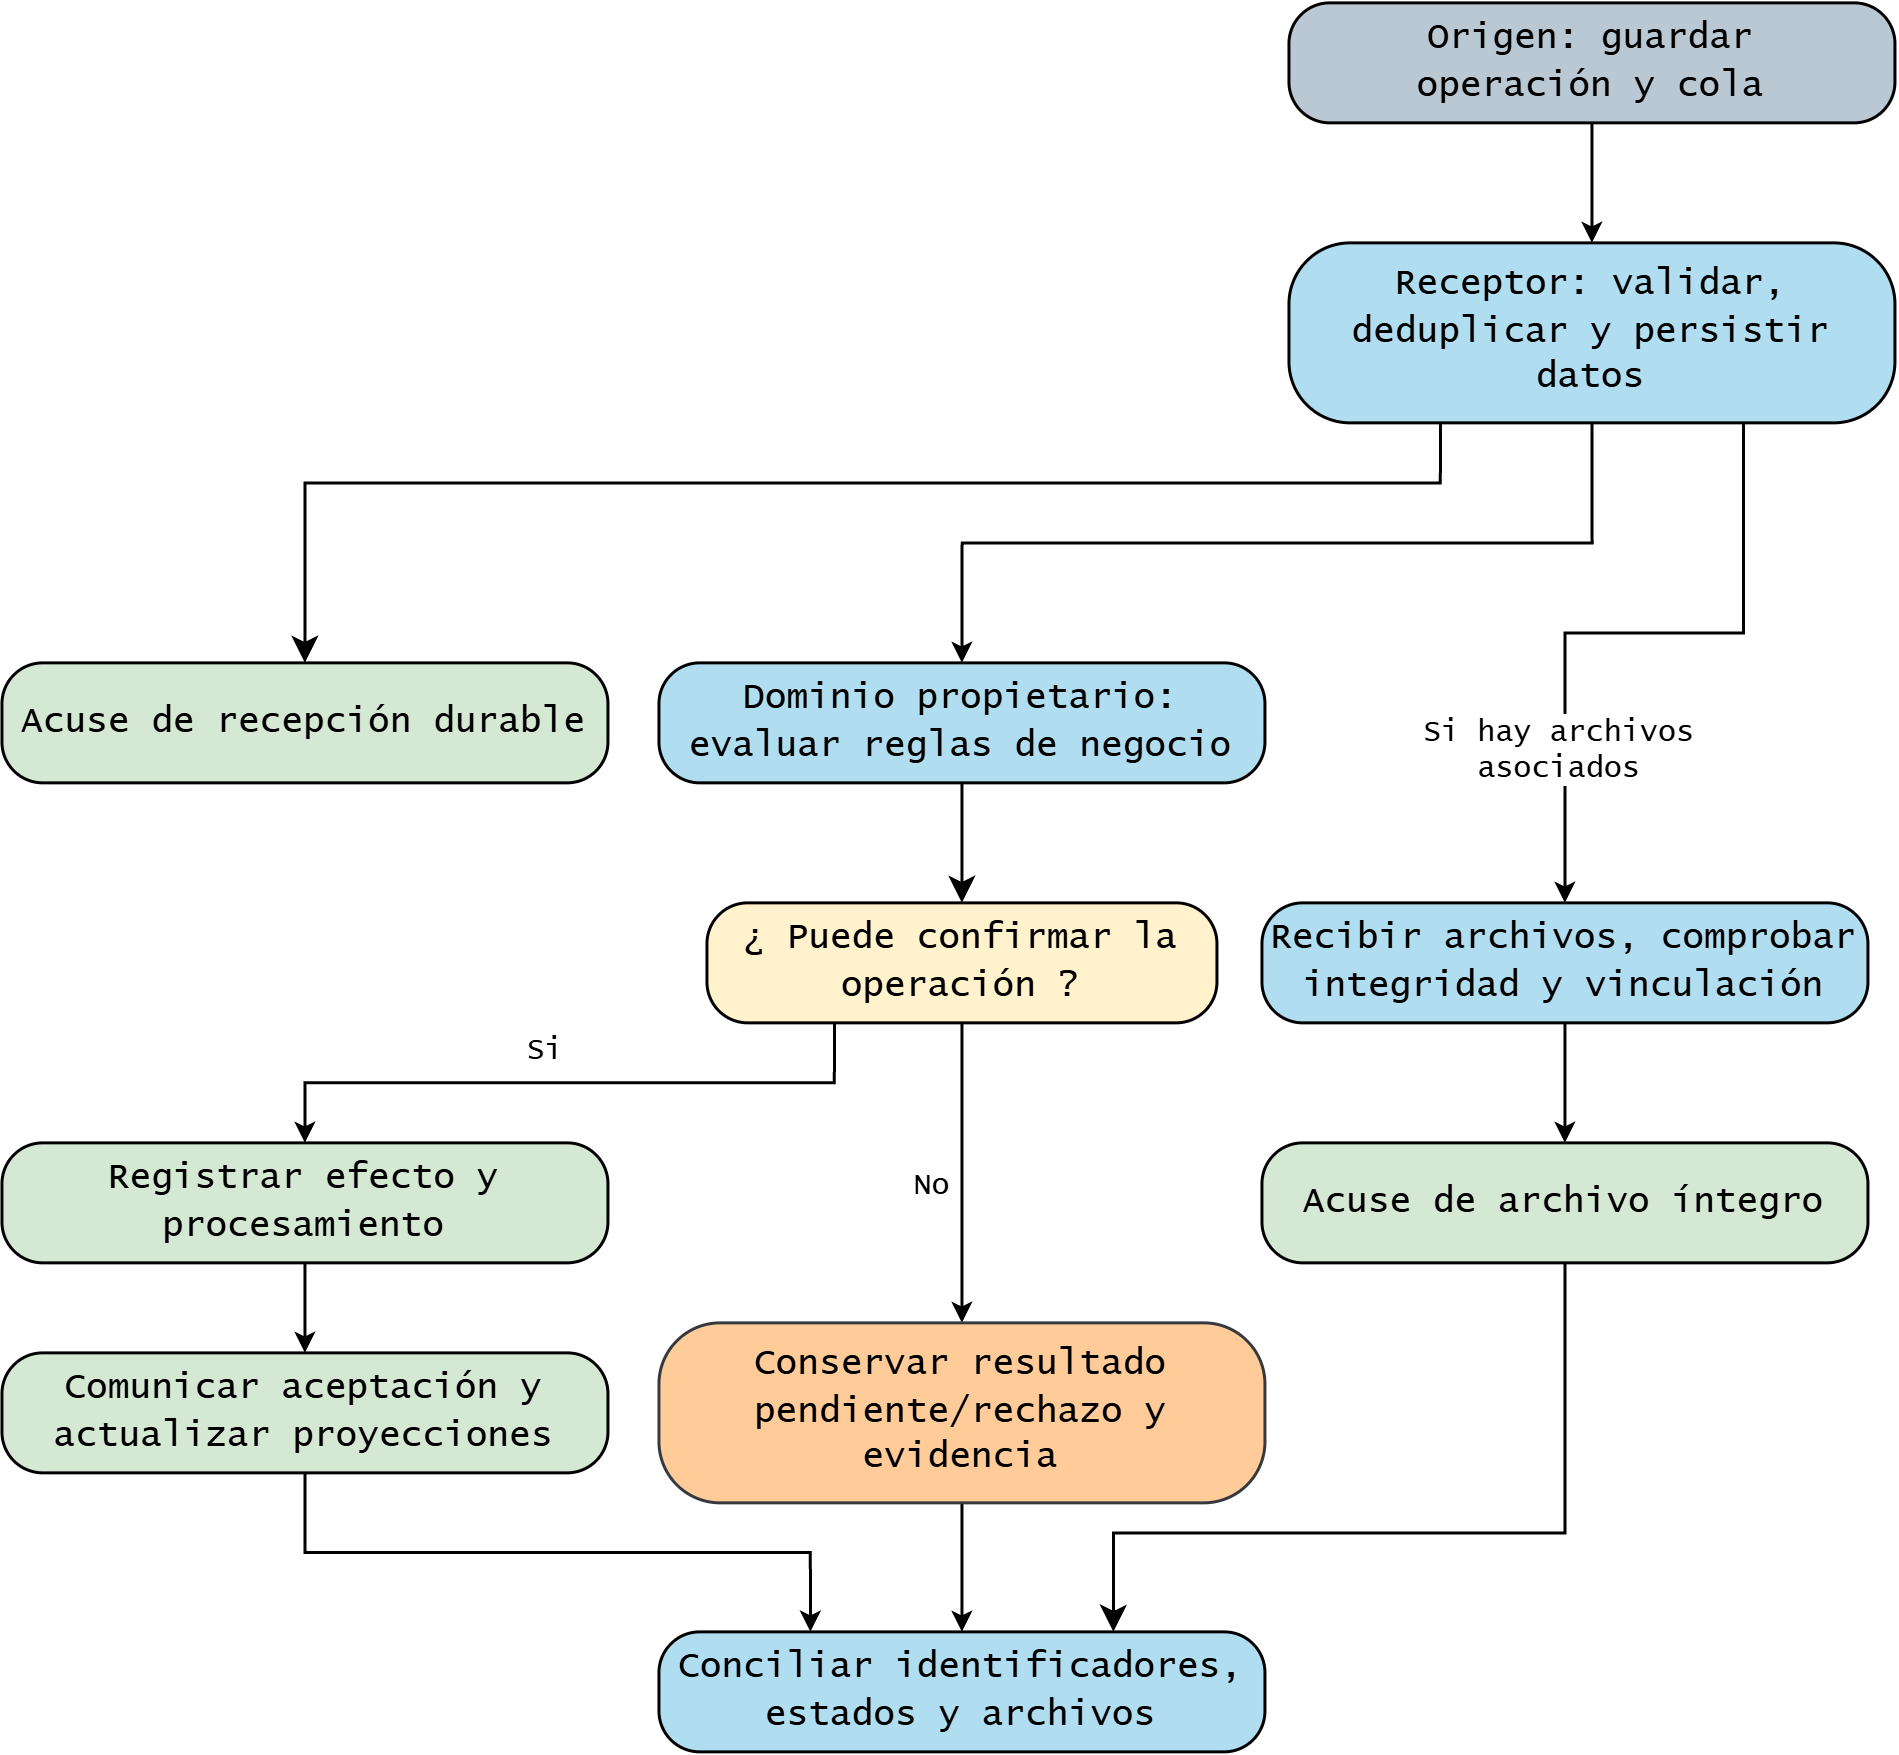
\includegraphics[width=\linewidth]{figuras/F5_13.png}
    }
    \caption{Persistencia, recepción y aceptación durante la sincronización}
    \label{fig:sincronizacion}
    \FuenteFigura{Flujo de sincronización de Synaptix; persistencia, acuses y aceptación descritos en esta sección.}
\end{figure}
\newpage

El primer acuse acredita conservación durable en el receptor; no acredita que las reglas de negocio hayan aceptado la operación. La autoridad emite un resultado independiente, y la recepción íntegra de archivos tiene su propia comprobación. Los reintentos conservan estos resultados sin repetir efectos. Una discrepancia sigue visible hasta su resolución y un expediente con archivos obligatorios faltantes no se declara íntegro. Las flechas representan pasos lógicos y no una transacción distribuida entre equipos.

La revisión humana de una discrepancia no es condición para transferir e incorporar automáticamente los registros válidos. Al cumplirse el plazo de sincronización, los hechos críticos deben estar persistidos y reflejados en un estado coherente, incluido un estado explícito de discrepancia cuando la evidencia no permita otra conclusión. No se informará ``sincronización completa'' si faltan registros del lote. Las fotografías pueden transferirse con prioridad posterior, como plantea SD4, pero un expediente no se declara íntegro mientras falte evidencia obligatoria; su atraso se mide por separado y no justifica demorar un dato requerido para el control operacional.

Las pruebas simulan la desconexión completa, trabajo nuevo durante la reconexión, mensajes repetidos, desorden, reinicio del proceso, archivo incompleto y falla tras confirmar una transacción pero antes del acuse. Se comprueban igualdad de conjuntos de identificadores, ausencia de efectos duplicados, conciliación de secuencias y tiempo extremo a extremo. La duración se mide desde la restitución efectiva del enlace hasta la convergencia operacional del conjunto acumulado. La capacidad y el ancho de banda se fundamentan en 5.4; el margen nominal del enlace no constituye por sí solo una prueba de cumplimiento.

\subsection{Almacenamiento transaccional y analítico}
\label{subsec:sd5_analitica}

El almacenamiento transaccional conserva el estado autorizado y sus eventos. La explotación histórica utiliza conjuntos derivados independientes, sin ejecutar consultas analíticas libres sobre la base operacional. Se mantiene el camino Parquet sobre S3 y consulta mediante Athena definido en SD4; Athena permite consultar datos en S3 mediante SQL (Amazon Web Services, s.\,f.-a). Los permisos, presupuesto de ejecución y concurrencia de los procesos analíticos se separan de los servicios críticos, conforme a BT RT-05.05.

\textbf{Flujo y modelo de explotación:} cada dominio publica hechos o extracciones incrementales mediante sus contratos, sin permitir que el extractor consulte esquemas ajenos. Los lotes incluyen versión, período, marcas de avance, cantidades y sumas de control. Una zona de recepción conserva la evidencia del lote; la validación produce conjuntos conciliados y posteriormente tablas de hechos y dimensiones. Una corrección tardía genera una versión del período afectado y mantiene trazabilidad del cambio; no sustituye silenciosamente un informe ya emitido.

El modelo semántico distingue hechos de navegación, intervalos de ocupación, participación escolar, servicios, despachos, consumos y movimientos de residuos. Sus dimensiones incluyen tiempo, ubicación, servicio y activo; los identificadores de personas se seudonimizan o excluyen cuando no son necesarios. Cada medida especifica unidad, numerador, denominador, filtros, exclusiones y estado de consolidación. Por ejemplo, recaladas no equivale a embarcaciones únicas; una matrícula no equivale a presencia en el agua; y un hecho facturable no equivale a ingreso cobrado. El saldo y los pagos provienen de contabilidad, conservando su fecha de origen.

\textbf{Información operacional oportuna:} la separación de cargas no permite enviar todas las consultas a un proceso por lotes. El estado inmediato se obtiene mediante proyecciones operacionales acotadas y mantenidas por los dominios, consultadas por sus servicios. Para las vistas derivadas de alta frecuencia se propone un almacén PostgreSQL de lectura con recursos separados del primario transaccional, alimentado por eventos; constituye una precisión de despliegue que debe incorporarse al dimensionamiento de SD4 y a los costos. La consulta de confirmación de una acción crítica verifica además la versión de su autoridad, evitando decidir a partir de una proyección atrasada.

La Figura~\ref{fig:explotacion} distingue las rutas de lectura operacional y explotación histórica. Ambas parten de contratos del propietario, pero tienen propósitos y condiciones de publicación diferentes.

\begin{figure}[htbp]
    \centering
    \makebox[\linewidth][c]{%
        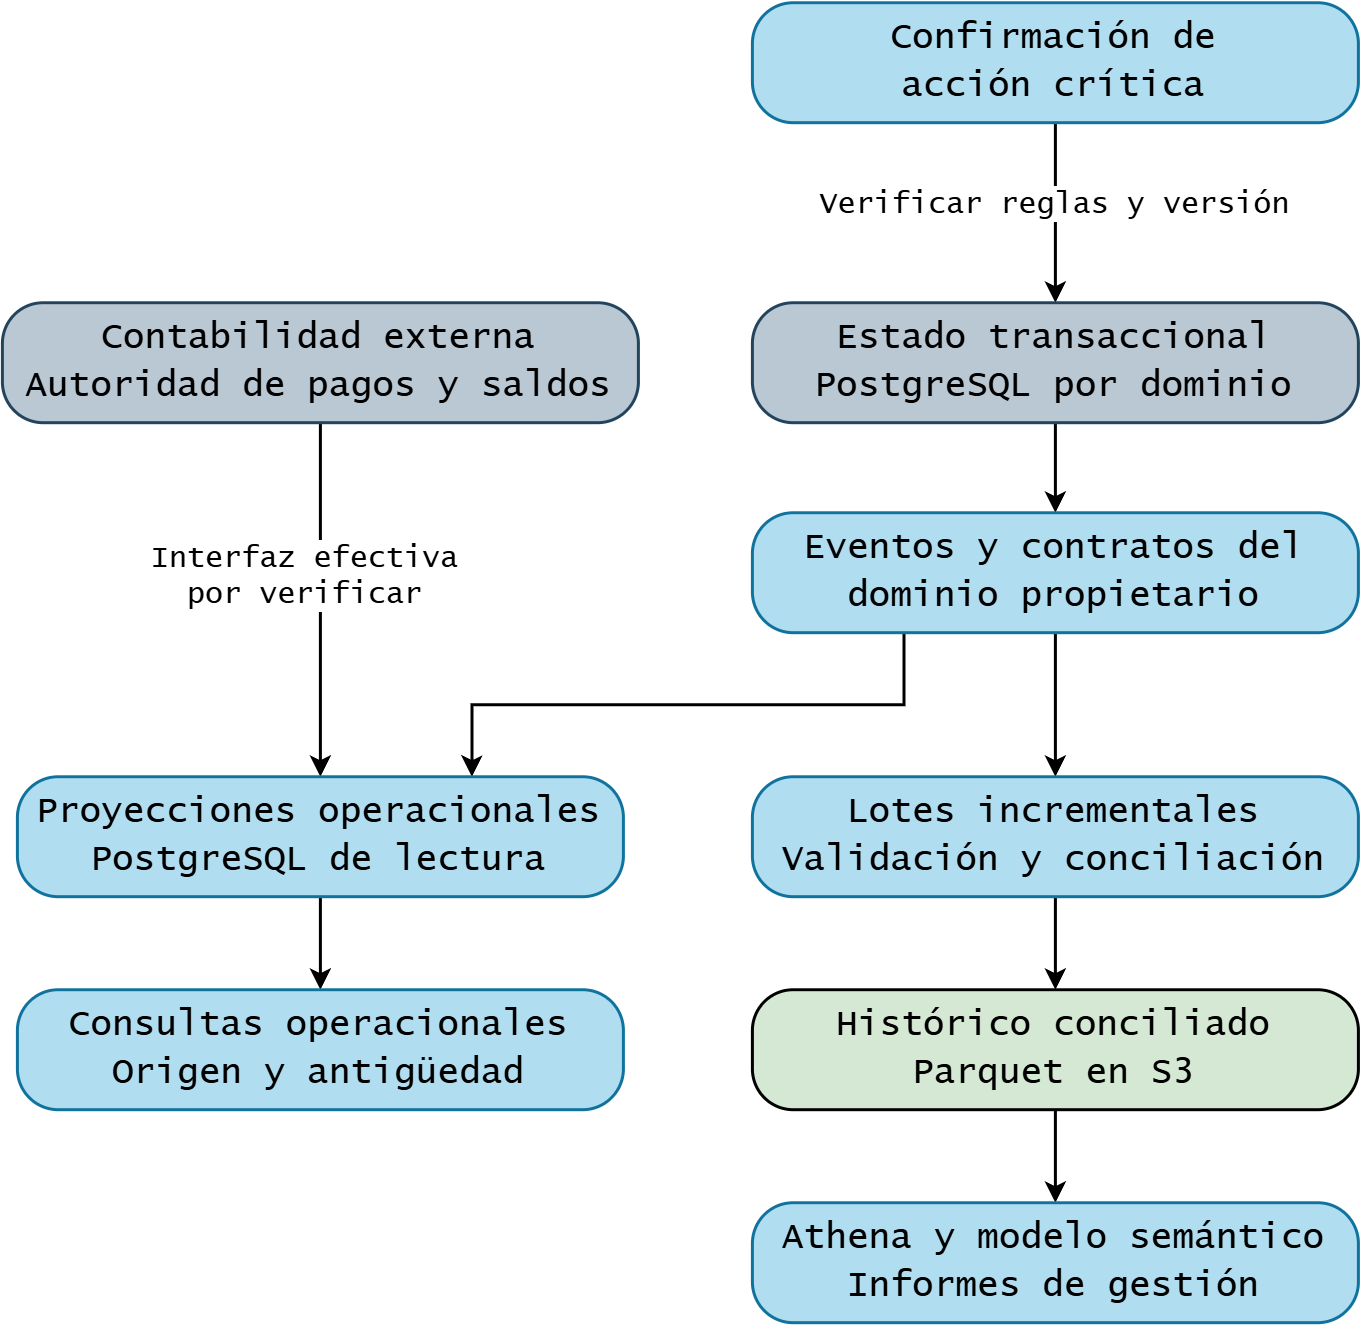
\includegraphics[width=0.8 \linewidth ]{figuras/F5_14.png}
    }
    \caption{Separación de la explotación operacional y la analítica histórica}
    \label{fig:explotacion}
    \FuenteFigura{Arquitectura de persistencia de Synaptix; separación transaccional y analítica descrita en esta sección.}
\end{figure}
\newpage

La ruta operacional publica proyecciones para consultas frecuentes, mientras la histórica valida y concilia lotes antes de exponerlos al modelo semántico. Una proyección no se transforma en maestro ni confirma acciones críticas por sí sola. Los documentos y evidencias originales almacenados en S3 constituyen un conjunto distinto de los archivos Parquet derivados: ambos conservan identificación, permisos y ciclo de vida según su finalidad. La actualización de pagos y saldos requiere además el contrato efectivo de contabilidad externa descrito más adelante.

La Tabla~\ref{tab:sd5_latencias} conserva los niveles de oportunidad exigidos por el caso. El término ``tiempo real'' no se reemplaza por un plazo inventado: el diseño debe reflejar cada confirmación en la vista correspondiente y medir su demora extremo a extremo, sin esperar una consolidación periódica.

\begingroup
\setlength{\tabcolsep}{3pt}
\begin{longtable}{@{}L{.28\textwidth}L{.40\textwidth}L{\dimexpr.32\textwidth-12pt\relax}@{}}
\caption{Oportunidad exigida y ruta de actualización}\label{tab:sd5_latencias}\\
\hline
\EncabezadoTabla{Información} & \EncabezadoTabla{Exigencia de C07 RT-05.29} & \EncabezadoTabla{Ruta prevista} \\ \hline
\endfirsthead
\hline
\EncabezadoTabla{Información} & \EncabezadoTabla{Exigencia de C07 RT-05.29} & \EncabezadoTabla{Ruta prevista} \\ \hline
\endhead
Ocupación de amarra & No superior a 60 segundos & Eventos operacionales \\ \addlinespace \hline
Consumo acumulado por amarra & Actualización al menos horaria & Acumulados de 15 minutos \\ \addlinespace \hline
Estado de cuenta & En tiempo real & Interfaz contable efectiva \\ \addlinespace \hline
Situación escolar & En tiempo real, sin excepción & Participación confirmada \\ \addlinespace \hline
Indicadores ambientales & Consolidación diaria & Cierre conciliado \\ \addlinespace \hline
\end{longtable}
\FuenteTabla{C07 RT-05.29; SD4 DA-09. Las rutas corresponden al diseño de Synaptix.}
\endgroup

Una interrupción de comunicaciones impide asegurar actualidad remota del hecho aún no recibido. La interfaz identifica cobertura, última confirmación y elementos pendientes; no presenta la última copia como realidad actual. En la escuela, la persistencia offline no basta para conocer inmediatamente hechos de otro dispositivo: la coordinación entre monitor, portería y autoridad local debe mantener el control efectivo de personas, según el flujo de 5.1.2. El contrato de actualización del saldo externo y los escenarios de operación escolar deben verificarse con SD3/SD4/SD9. Registrar una limitación técnica no rebaja las exigencias del caso ni acredita su cumplimiento.

El cliente dispondrá de informes de autoservicio sobre el modelo semántico publicado, con filtros de período, ubicación y servicio, profundización hasta el hecho autorizado, exportación abierta y programación por calendario. Las fórmulas y cambios de indicadores se versionan. El linaje se conserva al menos mediante identificadores de origen, lotes y transformaciones documentadas; la automatización integral del catálogo se trata como mejora deseable de BT RT-05.10, sin confundirla con los controles obligatorios de trazabilidad y calidad.

\textbf{Exportación íntegra y autónoma:} además de los informes, la solución permite al perfil autorizado del cliente exportar toda su información, en cualquier momento contractual, sin intervención de Synaptix ni cobro adicional, conforme a BT RT-05.06. El paquete contiene tablas en CSV UTF-8, eventos y estructuras en JSON/JSON Lines, conjuntos analíticos en Parquet cuando corresponda, archivos en sus formatos originales y metadatos documentados. Incluye diccionario, relaciones, versiones, unidades, zona temporal, clasificaciones, huellas y manifiesto de cantidades; no se limita a lo visible en una pantalla.

La exportación se ejecuta de forma asíncrona sobre instantáneas o cortes identificables por dominio y puntos de avance, declarando referencias pendientes o diferencias temporales entre fuentes. No se promete una instantánea global simultánea durante una partición. Un modo completo incorpora los registros pendientes al restablecerse la comunicación; un paquete solicitado antes indica expresamente su cobertura. La entrega se cifra y autoriza con autenticación reforzada; las claves de infraestructura y credenciales de terceros no forman parte del contenido exportable. Para evitar dependencia del proveedor, los datos se entregan legibles dentro de un paquete cifrado con acceso controlado por el cliente. La prueba de portabilidad comprueba cantidades, relaciones y lectura en un entorno independiente.

\subsection{Calidad y gobierno de datos}
\label{subsec:sd5_calidad}

La calidad se gestiona desde la captura hasta la explotación, considerando completitud, exactitud y consistencia conforme a la exigencia de BT RT-05.04. La gestión conforme a ISO/IEC 25012 es una exigencia de la base y se operacionaliza mediante reglas, métricas y evidencias; esta formulación no constituye una certificación del diseño. Las reglas de calidad se implementan por dominio y se documentan junto al atributo, su fuente y el efecto de un incumplimiento. El criterio es impedir decisiones incorrectas sin ocultar hechos ocurridos.

\textbf{Validación y tratamiento de defectos:} en captura se verifican formato, obligatoriedad condicional, unidad, intervalo temporal, referencia conocida, autorización y transición de estado. En recepción se verifican identidad técnica, esquema, secuencia e integridad. Antes de publicar un consumo o hecho facturable se valida la asociación y se comprueba que no exista un efecto anterior para el mismo origen. Los defectos se clasifican como bloqueantes para la decisión, advertencias o incidencias que permiten conservar el hecho con uso restringido. Una lectura inválida no genera cargo, pero conserva su evidencia; una embarcación no identificada no se elimina del registro de presencia.

Cada incidencia posee identificador, dominio, regla incumplida, registros afectados, fecha, severidad, responsable, plazo propuesto y estado de resolución. El responsable funcional determina la corrección de negocio; el equipo técnico de Synaptix ejecuta reparaciones, transformaciones y reprocesos autorizados. La resolución registra el antes y después, su fundamento y los consumidores afectados. Si una corrección cambia un indicador o una exportación ya generada, se publica una revisión identificable.

Los indicadores de la Tabla~\ref{tab:sd5_calidad_indicadores} se calculan sobre universos explícitos y períodos definidos. Una población vacía se informa como ``no aplica'', no como cumplimiento total. Los registros pendientes no se excluyen del denominador sin una regla visible. Las metas de aceptación son propuestas de diseño y se distinguen de los plazos establecidos por las bases.

\begingroup
\setlength{\tabcolsep}{3pt}
\begin{longtable}{@{}L{.27\textwidth}L{.43\textwidth}L{\dimexpr.30\textwidth-12pt\relax}@{}}
\caption{Indicadores de calidad y metas de diseño}\label{tab:sd5_calidad_indicadores}\\
\hline
\EncabezadoTabla{Indicador} & \EncabezadoTabla{Razón o conteo} & \EncabezadoTabla{Meta propuesta} \\ \hline
\endfirsthead
\hline
\EncabezadoTabla{Indicador} & \EncabezadoTabla{Razón o conteo} & \EncabezadoTabla{Meta propuesta} \\ \hline
\endhead
Completitud & $N_{\mathrm{válidos}}/N_{\mathrm{aplicables}}$ & 100\,\% al confirmar \\ \addlinespace \hline
Exactitud & $N_{\mathrm{coincidentes}}/N_{\mathrm{contrastados}}$ & Cero diferencias críticas \\ \addlinespace \hline
Consistencia & $N_{\mathrm{conformes}}/N_{\mathrm{evaluados}}$ & Cero contradicciones críticas \\ \addlinespace \hline
Unicidad de efectos & $N_{\mathrm{efectos\ indebidos}}$ & Cero \\ \addlinespace \hline
Oportunidad & $N_{\mathrm{en\ plazo}}/N_{\mathrm{exigibles}}$ & Plazos de C07 \\ \addlinespace \hline
Integridad de sincronización & $N_{\mathrm{recibidos}}/N_{\mathrm{manifestados}}$ & 100\,\% de registros críticos \\ \addlinespace \hline
\end{longtable}
\FuenteTabla{Criterios de calidad de datos de Synaptix conforme a BT RT-05.04 y C07 RT-03.13/RT-05.29; metas por verificar con SD9.}
\endgroup

En completitud se cuentan campos obligatorios aplicables, según el estado y la actuación evaluados; un campo opcional no integra ese denominador. En exactitud se contrastan valores con evidencia independiente dentro de una muestra cuya población, selección y tamaño quedan registrados. Validar el formato de un dato no prueba su exactitud. En consistencia se cuentan registros sometidos a reglas identificadas, conservando el detalle de las reglas fallidas. Las razones se expresan como porcentaje multiplicándolas por cien, sin mezclar universos entre períodos.

Para el control propuesto, un defecto crítico es aquel que puede habilitar una actuación insegura, una autorización incompatible, pérdida de evidencia obligatoria o un efecto económico incorrecto. Por ejemplo, confirmar una entrega escolar sin autorización vigente, aceptar dos asignaciones incompatibles de una misma amarra o generar consumo facturable desde una asociación medidor--amarra inválida bloquea la decisión correspondiente. El dato y su evidencia se conservan para resolución, sin convertir el bloqueo en pérdida de registros.

La oportunidad usa los resultados exigibles del período, incluidos los pendientes, y mide también demora máxima y antigüedad. La integridad de sincronización compara conjuntos de identificadores críticos del manifiesto con los recibidos; un porcentaje de recepción no sustituye el control separado de efectos duplicados. El diccionario A5.1 y la especificación de pruebas SD9 deben mantener la correspondencia entre característica de calidad, regla, población, métrica y evidencia. Estos ejemplos desarrollan el método, sin acreditar que los anexos o las pruebas ya estén completos.

El tablero de calidad se habilita al cliente con acceso según función. Presenta tendencia, población evaluada, reglas ejecutadas, registros pendientes, antigüedad de defectos, última sincronización y responsable. Las alertas de pérdida, duplicación o contradicción de seguridad se emiten al detectarse; la revisión consolidada se propone diaria en operación y antes de cada cierre contable o ambiental. Los indicadores agregados no exponen nombres de menores, antecedentes de salud ni deuda a perfiles sin autorización.

\textbf{Gobierno y cambios:} cada dominio tiene un responsable funcional y un custodio técnico. La administración del cliente aprueba criterios comerciales; operaciones valida estados y asignaciones; escuela valida participación y autorizaciones; mantenimiento valida activos; y los responsables de seguridad autorizan políticas de acceso. Synaptix mantiene los procesos técnicos, respaldos, controles, tableros y soporte. DEC-22 y la organización de SD6/SD7 deben reflejar estas funciones y suplencias; no se asigna al cliente administración de bases de datos.

Los cambios de catálogo o parámetro conservan versión, vigencia, motivo, solicitante y aprobador. Los de impacto operacional requieren segundo perfil conforme a BT RT-16.03 y no pueden rebajar límites exigidos por el caso. Las modificaciones de esquema siguen compatibilidad progresiva: incorporar, migrar y verificar antes de retirar campos. El despliegue conserva un camino de reversión de aplicación y datos comprobado en Preproducción; no se promete reversibilidad automática de una transformación destructiva. Se bloquea una promoción con pérdida de referencias, reglas críticas fallidas o migración sin conciliación.

\subsection{Protección y ciclo de vida}
\label{subsec:sd5_proteccion}

La protección se define por finalidad, relación con la persona o entidad y etapa de vida del registro. Se distinguen datos operacionales, personales restringidos, sensibles y evidencia sujeta a conservación. La clasificación se aplica a atributos y documentos, no solo al nombre de la tabla. C07 RT-11.10 exige cifrado a nivel de campo para salud, datos personales de menores, armadores, tripulantes y trabajadores contratistas, y posición de embarcación compartida con consentimiento. El cifrado del disco o del almacén no sustituye esa exigencia.

\textbf{Acceso mínimo, consentimiento y auditoría:} las autorizaciones combinan identidad, rol, dominio, relación vigente, finalidad y estado del dispositivo. Un monitor accede a la nómina y antecedentes mínimos necesarios para su clase; portería verifica autorización y entrega sin recibir la ficha de salud completa; administración consulta los antecedentes económicos de su función; y un contratista accede a su personal y faenas autorizadas. Se evita copiar identificadores personales en nombres de objetos, mensajes de error, trazas o tableros generales. Desarrollo y pruebas emplean datos sintéticos o tratados para impedir identificación indebida.

Los campos restringidos se cifran en aplicación con claves de datos protegidas por el mecanismo de gestión de claves de SD4. La especificación de seguridad de SD4 debe identificar el algoritmo, la versión de clave asociada a cada campo cifrado, la política de rotación y la separación de funciones de custodia. Esta referencia exige una definición verificable en ese documento; no se presenta un algoritmo todavía no fijado como acuerdo del equipo. La rotación conserva la capacidad de lectura de versiones durante su retención. En dispositivos solo se distribuye el subconjunto necesario, cifrado y vinculado a identidad y permiso vigentes; las claves no se almacenan en texto claro ni se incluyen en la aplicación. El permiso offline de DA-16, con renovación diaria y vigencia máxima de 72 horas, es una decisión arquitectónica distinta de las autonomías de 24, 12 y 8 horas del caso. Su vencimiento deniega nuevas acciones fuera del procedimiento de contingencia autorizado.

El consentimiento identifica titular, representante cuando proceda, finalidad, datos autorizados, versión de información entregada, fecha, canal y evidencia de otorgamiento o revocación. El plan voluntario y la posición consentida de una embarcación no se convierten en condición obligatoria para todos los armadores. La revocación detiene los nuevos tratamientos dependientes de ese consentimiento y propaga la restricción a consumidores, exportaciones futuras y copias operacionales. No elimina automáticamente evidencias cuya conservación esté exigida; el registro distingue la finalidad terminada de la obligación de conservar.

Con enlace, la revocación se aplica y distribuye inmediatamente. En equipos incomunicados no se afirma recepción instantánea: se limita la exposición mediante vigencia, alcance mínimo y caducidad local, y se aplica la revocación antes de reanudar el servicio al reconectar. Los tratamientos voluntarios de posición no se habilitan offline por la sola existencia de un permiso general del dispositivo. El consentimiento y la política vigentes deben autorizar específicamente su finalidad.

La auditoría registra creación, modificación, eliminación y consultas sensibles, con sujeto, instante, dispositivo, finalidad, entidad, resultado, versión de política y correlación. Incluye accesos a salud, menores, posición consentida y antecedentes de deuda, conforme a C07 RT-16.09. Los valores anteriores y posteriores necesarios para BT RT-05.03 se conservan cifrados en evidencia restringida, separados de los registros técnicos generales. Los cambios de auditoría generan nuevas evidencias; ningún perfil administrativo dispone de una función para alterar el historial protegido.

Se propone sellar los lotes de auditoría con manifiestos e integridad verificable y conservarlos en el repositorio separado previsto por SD4. Para evidencia con plazo definido se aplica Object Lock en modo de cumplimiento cuando corresponda a la política aprobada: su protección actúa sobre versiones de objetos y limita su eliminación durante la retención. Una retención o bloqueo vigente debe resolverse por su procedimiento de conservación, no mediante un intento de borrado anticipado (Amazon Web Services, s.\,f.-b). La huella de integridad ayuda a detectar alteraciones, pero no reemplaza la evidencia de autor, permisos ni firma cuando esta sea exigible.

\textbf{Retención y archivado:} la Tabla~\ref{tab:sd5_retencion} sintetiza los plazos expresos de las bases. Los criterios complementarios del diseño se explican a continuación. Cuando la fuente no precisa el inicio del cómputo, se propone un evento de referencia conservador y se registra como decisión de política. La matriz A5.2 debe materializar estas reglas por entidad y atributo; no puede reducirlas por razones de costo o capacidad.

\begingroup
\setlength{\tabcolsep}{3pt}
\begin{longtable}{@{}L{.53\textwidth}L{.29\textwidth}L{\dimexpr.18\textwidth-12pt\relax}@{}}
\caption{Síntesis de las retenciones exigidas por las bases}\label{tab:sd5_retencion}\\
\hline
\EncabezadoTabla{Categoría} & \EncabezadoTabla{Plazo} & \EncabezadoTabla{Fuente} \\ \hline
\endfirsthead
\hline
\EncabezadoTabla{Categoría} & \EncabezadoTabla{Plazo} & \EncabezadoTabla{Fuente} \\ \hline
\endhead
Escuela: menores, autorizaciones y salud & Hasta 23 años; mínimo 10 años & C07 RT-05.10 \\ \addlinespace \hline
Salida, regreso y antecedentes de zarpe & 5 años & C07 RT-05.10 \\ \addlinespace \hline
Contratos de amarra, custodia y estado de cuenta & 6 años & C07 RT-05.10 \\ \addlinespace \hline
Residuos peligrosos y actas de derrame & 6 años & C07 RT-05.10 \\ \addlinespace \hline
Series de consumo por amarra & 5 años & C07 RT-05.10 \\ \addlinespace \hline
Inspección de trenes de fondeo & Vida útil + 5 años & C07 RT-05.10 \\ \addlinespace \hline
Despacho de combustible & 5 años & C07 RT-05.10 \\ \addlinespace \hline
Videovigilancia & 6 meses & C07 RT-05.10 \\ \addlinespace \hline
Auditoría & Al menos 5 años & BT RT-16.10 \\ \addlinespace \hline
Eventos técnicos de seguridad & 12 meses + 24 en archivo & BT RT-11.14 \\ \addlinespace \hline
\end{longtable}
\FuenteTabla{C07 RT-05.10; BT RT-16.10 y RT-11.14. El detalle de cómputos y bloqueos se especifica mediante A5.2.}
\endgroup

La síntesis diferencia archivo documental de registros técnicos. Los eventos de seguridad permanecen al menos doce meses en línea y veinticuatro adicionales en archivo recuperable. La auditoría se conserva al menos cinco años y por el plazo mayor cuando respalda un expediente cuya conservación lo requiere. El video permanece en la plataforma existente; una evidencia extraída y vinculada a un expediente sigue la regla de ese expediente.

Como cómputos de diseño, se adopta cierre del episodio para salida, regreso y zarpe; término contractual para contratos de amarra; cierre de custodia o fecha del estado para sus antecedentes; cierre del registro o incidente para residuos y derrames; período de consumo para sus series; y fecha del despacho para combustible. El plazo adicional de las inspecciones de trenes de fondeo comienza al término de la vida útil del elemento. Ninguno de estos eventos de inicio se atribuye como cita literal a una base que no lo precise.

Las faenas, planes de trabajo y acreditaciones de contratistas se conservan, como política propuesta, seis años desde el cierre de la faena o el término de vigencia correspondiente. Los registros escolares de adultos tienen una propuesta de cinco años desde el cierre, salvo obligación de plazo mayor. Los avisos independientes tienen una propuesta de cinco años. Maestros, contactos y consentimientos mantienen su vigencia y el plazo de los hechos que respaldan; el término de una finalidad no elimina evidencias todavía necesarias para otra obligación.

La matriz A5.2 debe vincular estas reglas con los nueve dominios y sus categorías, incluidos planes voluntarios de navegación, ocupación e inspección de boyas y autorizaciones. Para cada categoría se especifican evento de inicio, vencimiento, bloqueo, archivo, repositorios y responsable. Una categoría sin correspondencia explícita queda pendiente de definición y no se incorpora a una purga automática. La descripción de esta matriz no acredita que su detalle ya esté completado.

Los objetos y atributos de una misma categoría heredan una regla versionada de vencimiento. Para un expediente de menor, la fecha propuesta de eliminación elegible es la posterior entre su cumpleaños número 23 y el cierre más diez años, siempre que no exista bloqueo. Una fecha de nacimiento desconocida impide calcular el vencimiento: genera una incidencia y revisión, no una eliminación automática. Las 14 embarcaciones abandonadas mantienen la totalidad de su expediente y las restricciones de conservación mientras exista una actuación o controversia pendiente. La retención no autoriza por sí sola una medida de cobro o disposición del bien.

Se propone mantener en consulta operacional los registros activos y los últimos doce meses de registros cerrados; el resto pasa a archivo consultable hasta su vencimiento, conservando índice, permisos, relaciones y comprobación de integridad. Este cambio de nivel no borra información ni altera los períodos de migración de 5.3. Los documentos necesarios para la operación siguen disponibles aunque sean antiguos. La recuperación de evidencia archivada se plantea como tarea asíncrona con objetivo de hasta cuatro horas para solicitudes ordinarias; los expedientes activos y críticos quedan en acceso inmediato. Son criterios operacionales propuestos que deben reflejarse en capacidad, costos y pruebas.

Las muestras de medición por minuto no se confunden con la serie consolidada cada quince minutos. Se propone conservar el detalle local durante treinta días y, antes de su purga, verificar la persistencia central de los extremos acumulativos, época, secuencias, asociación y reglas que permiten reconstruir el consumo de cada intervalo. Se conservan por cinco años esas bases de cálculo y las muestras adicionales que sustenten anomalías o rectificaciones. Una muestra vinculada a una incidencia abierta no se purga por antigüedad. Esta propuesta limita crecimiento sin eliminar el respaldo del consumo; debe conciliarse con la volumetría de 5.4 y SD4.

\textbf{Eliminación verificable:} la eliminación se ejecuta mediante una tarea controlada que selecciona registros vencidos, consulta bloqueos, comprueba dependencias y genera una lista revisable. La autorización se separa de la ejecución técnica; el vencimiento de una regla inmutable aprobada habilita el procedimiento, no una edición discrecional del historial. Se eliminan datos elegibles en bases, objetos y versiones, índices de búsqueda, conjuntos analíticos, exportaciones temporales y cachés administradas. Se registran categoría, cantidades, regla, fecha, responsable y resultado sin reproducir el contenido eliminado. Las fallas generan una incidencia hasta completar la propagación.

Para las copias fuera de línea se conserva una orden de eliminación que debe aplicarse al reconectar antes de habilitar acceso a datos vencidos. La caché de dispositivo se depura tras aceptación durable de los hechos y al concluir la necesidad operacional; un registro no sincronizado no se borra por el simple vencimiento de una ventana de caché. Las exportaciones bajo control de la plataforma caducan a los siete días como propuesta; las ya descargadas por el cliente quedan registradas como entregas y sujetas a su custodia, sin prometer borrado remoto de copias que el sistema ya no controla.

Los respaldos se gestionan separadamente de la retención documental. SD4 fija recuperación a un punto en el tiempo de 35 días y copias mensuales, pero no define aquí la permanencia de estas últimas. Se propone una rotación de doce copias mensuales cifradas para recuperación, distinta del archivo documental de largo plazo. Cada copia tiene fecha de expiración y acceso exclusivo de recuperación. Una restauración se efectúa en un entorno aislado, reaplica el registro vigente de eliminaciones y revocaciones, y se concilia antes de habilitar usuarios. La recuperación de RDS a un punto en el tiempo crea una instancia de destino, lo que permite preparar esta comprobación antes de sustituir el servicio (Amazon Web Services, s.\,f.-c).

Para los nueve dominios se propone respaldo automático diario, continuidad de registros para la recuperación a un punto en el tiempo en nube durante 35 días y copia mensual con la rotación indicada. En el recinto se propone copia diaria cifrada con 30 días de retención y envío fuera del sitio al disponer de enlace, complementando la réplica síncrona de SD4. Los objetos conservan versiones protegidas y copias fuera del sitio según su clasificación. Estos mecanismos deben integrarse al esquema 3-2-1-1-0 exigido por BT RT-07.09: contar réplicas no acredita por sí solo diversidad de medios ni protección contra corrupción. Se realiza una prueba de restauración mensual y se mide la recuperación de los dominios críticos contra el objetivo regional de cuatro horas de SD4; la estimación de restauración completa por dominio debe documentarse en 5.4/A5.4 conforme a BT RT-07.13, considerando preparación, transferencia, restauración, reaplicación de eliminaciones y conciliación. El objetivo regional no sustituye esas estimaciones ni sus mediciones posteriores. La recuperación analítica se secuencia después del servicio crítico, sin presentarla como incluida en un tiempo que aún no se ha medido.

La eliminación completa de una categoría solo se declara cuando las copias residuales han vencido o han sido destruidas de forma verificable; hasta entonces se informa su confinamiento y fecha prevista de expiración. No se utiliza la destrucción de una clave compartida como atajo si deja ilegibles registros que todavía deben conservarse. Los bloqueos de preservación suspenden la eliminación solo sobre su alcance justificado, con responsable, motivo, revisión y levantamiento registrados. Su duración no convierte toda la base en archivo perpetuo.

La validación con SD9 comprobará acceso indebido denegado, registro de consultas sensibles, revocación con y sin enlace, recuperación de versiones, integridad de archivo, eliminación propagada y restauración sin reaparición de datos vencidos. Las pruebas de sincronización, oportunidad y portabilidad de los apartados anteriores completan la evidencia de gestión. Estos controles son compromisos verificables de la propuesta; la redacción del diseño no acredita que las pruebas ya se hayan ejecutado.

%---------------------------------------------
\newpage
\section{Estrategia de migración} %5.3
La migración trasladará los antecedentes del sistema administrativo de 2014, las planillas y los expedientes del puerto a las estructuras definidas en 5.1. El proceso comprende extracción, saneamiento, carga, conciliación y cambio controlado de autoridad. La copia de archivos será una actividad de este proceso; la aceptación dependerá de comprobar que los antecedentes siguen siendo completos, interpretables y utilizables.

La estrategia conserva el alcance de SD2, apartado 2.5 y decisión DEC-02, y la implantación por procesos del SD3. Se aplican los requisitos de las Bases Técnicas Transversales sobre plan, perfilado, dos ensayos completos y conciliación cuantitativa, y el alcance histórico específico de las bases del caso (Pontificia Universidad Católica de Valparaíso [PUCV], 2026b, RT-05.11--RT-05.15; PUCV, 2026c, RT-05.15). Los procedimientos siguientes son el diseño de ejecución de Synaptix; los tiempos y volúmenes estimados se comprobarán en preproducción antes de autorizar un corte.

\subsection{Alcance de datos} %5.3.1

El alcance obligatorio y el período de conservación son dimensiones distintas. El sistema de origen contiene doce años de historia, pero el caso fija conjuntos y períodos concretos para la migración. Se inventariará toda esa historia para identificar qué se carga como dato operativo, qué se mantiene en consulta histórica y qué documentos respaldan un expediente vigente. La selección por antigüedad no podrá fragmentar los antecedentes de las catorce embarcaciones abandonadas ni retirar documentación necesaria para una actuación en curso.

La Tabla~\ref{tab:sd5_alcance_historico} establece la cobertura mínima por conjunto. El origen indicado identifica dónde se buscará la información; su existencia y estructura se comprobarán durante el inventario, sin suponer una interfaz de extracción disponible.

\begingroup
\setlength{\tabcolsep}{3pt}
\begin{longtable}{@{}L{.23\textwidth}L{.23\textwidth}L{.27\textwidth}L{\dimexpr.27\textwidth-18pt\relax}@{}}
\caption{Conjuntos incluidos en la migración}\label{tab:sd5_alcance_historico}\\
\hline
\EncabezadoTabla{Conjunto} & \EncabezadoTabla{Origen principal} & \EncabezadoTabla{Cobertura obligatoria} & \EncabezadoTabla{Destino funcional} \\ \hline
\endfirsthead
\hline
\EncabezadoTabla{Conjunto} & \EncabezadoTabla{Origen principal} & \EncabezadoTabla{Cobertura obligatoria} & \EncabezadoTabla{Destino funcional} \\ \hline
\endhead
Socios y armadores & Sistema 2014, padrones & Totalidad del padrón & Persona, Organización y vínculos \\ \addlinespace \hline
Contratos y documentos & Sistema 2014, carpetas & Todos los contratos vigentes y adjuntos & Contrato, partes y asignaciones \\ \addlinespace \hline
Pagos y saldos & Sistema 2014, contabilidad & Seis años de historia & Antecedentes financieros conciliados \\ \addlinespace \hline
Embarcaciones e invernadas & Sistema 2014, inventario & Totalidad del registro & Embarcación, ubicación e historial \\ \addlinespace \hline
Embarcaciones abandonadas & Sistema 2014, expedientes & 14 de 14, antecedentes completos & Expedientes y evidencia relacionada \\ \addlinespace \hline
Matrícula de escuela & Registros de escuela & Últimos tres años & Alumno, matrícula y relaciones \\ \addlinespace \hline
\end{longtable}
\FuenteTabla{PUCV (2026c, cap.~15, RT-05.15); correspondencia propuesta con el modelo de 5.1.}
\endgroup

La totalidad se comprobará contra manifiestos de origen y no contra las cifras actuales del caso. Los 1.240 socios y los 296 contratos permanentes sirven como referencias de escala, pero no determinan cuántas identidades, versiones o documentos existen en doce años. Las matrículas de tres años tampoco equivalen a tres padrones de personas distintas. Las relaciones entre alumno, apoderado y autorización se preservarán cuando formen parte del antecedente disponible; una autorización antigua no se convertirá en una autorización vigente por efecto de la carga.

Los antecedentes de otros procesos, como navegación, residuos, acreditación e inspección, se incorporarán desde sus fuentes cuando existan y deban conservarse conforme a 5.2.5. La ausencia de un registro se documentará como condición del origen. Los movimientos, pagos, autorizaciones y evidencias ambientales de una serie histórica se incorporarán únicamente con respaldo de las fuentes originales. La telemetría que se instale con el proyecto comenzará con una fecha de inicio identificada.

\textbf{Inventario y extracción:} el responsable de datos registrará cada fuente, custodio, ubicación, período, formato, número de registros, tamaño, sensibilidad y mecanismo de acceso autorizado. Administración comprobará los cierres y saldos; Escuela validará los antecedentes de alumnos; y Operaciones contrastará las embarcaciones, ubicaciones e invernadas con el inventario físico. El 22~\% de amarras mal asignadas descrito en el caso exige esta comprobación y no autoriza a corregir una asignación a partir de una planilla aislada.

Se obtendrá una copia autorizada del origen y se comprobará su integridad antes de analizarla. La extracción seguirá este orden: exportación nativa si conserva los datos y relaciones necesarios; lectura controlada de una copia de la base; y extracción supervisada de reportes para los antecedentes que no puedan recuperarse por los medios anteriores. No se presupone una API, un registro de cambios ni un proveedor capaz de explicar el modelo.

La falta de documentación se abordará examinando tablas, claves, relaciones y reportes en la copia. La persona que conoce el sistema demostrará los procesos de consulta, facturación y cierre, mientras Synaptix documentará sus entradas, resultados y reglas observables. La demostración ayudará a interpretar la información; no reemplazará las comprobaciones de recuentos y saldos.

La Figura~\ref{fig:ruta_migracion} representa los puntos de control desde el origen hasta el destino.

\begin{figure}[htbp]
    \centering
    \makebox[\linewidth][c]{%
        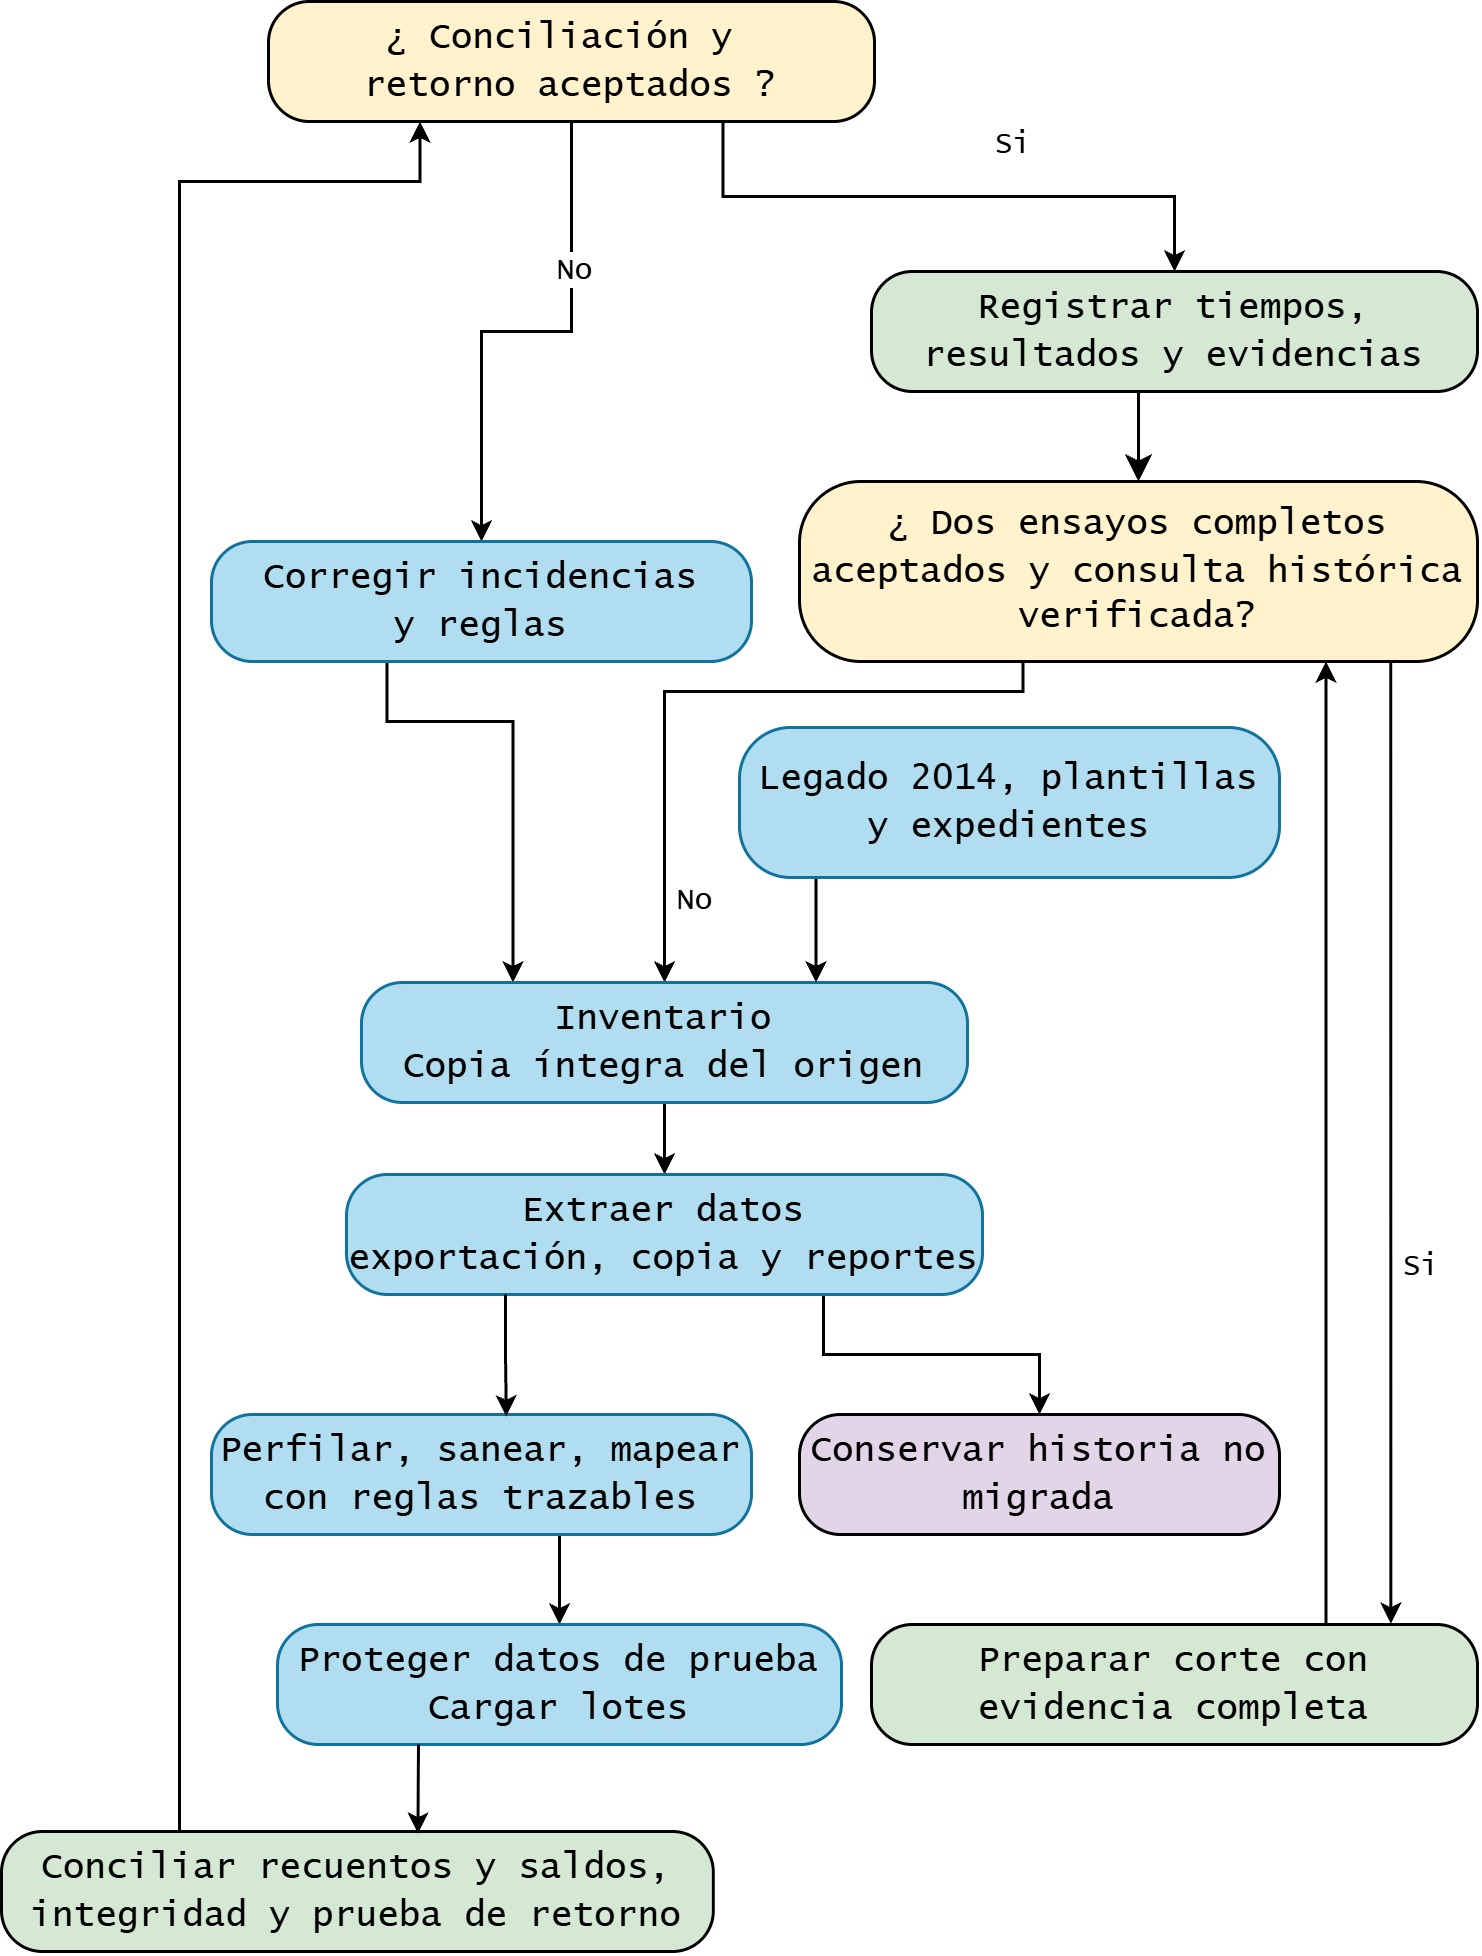
\includegraphics[width=0.9 \linewidth ]{figuras/F5_15.png}
    }
    \caption{Ruta controlada de migración}
    \label{fig:ruta_migracion}
    \FuenteFigura{Estrategia de migración de Synaptix; etapas y controles descritos en esta sección.}
\end{figure}
\newpage
%Fuente: PUCV (2026b, RT-05.11--RT-05.14

El recorrido mantiene la copia inicial sin modificaciones. Toda transformación deja una correspondencia verificable y toda carga produce un resultado conciliable. Una incidencia vuelve a la revisión de su regla y se reejecuta en un lote identificado; no se corrige manualmente el destino dejando el origen y la regla sin explicación.

\textbf{Perfilado, saneamiento y mapeo:} se identificarán campos vacíos, formatos inválidos, duplicados, referencias inexistentes, diferencias de unidad y contradicciones de vigencia. Cada defecto conservará fuente, valor original, regla aplicada, valor resultante, responsable y motivo. Los registros que no puedan aceptarse se mantendrán en una zona restringida de incidencias, incluidos en los recuentos del conjunto.

El mapeo por atributo documentará campo de origen, significado, entidad y atributo de destino, tipo, unidad, transformación, condición de obligatoriedad y control de aceptación. Se alineará con las definiciones de 5.1 y con la especificación del diccionario A5.1. Las conversiones de fechas distinguirán instantes de eventos de fechas administrativas: una fecha sin hora ni zona conocida no se transformará en un instante UTC supuestamente exacto. Importes y mediciones usarán decimales y unidades explícitas.

Los identificadores heredados se conservarán junto con su sistema emisor y su correspondencia con la identidad técnica de destino. La relación se generará una sola vez y se reutilizará en los reintentos. Coincidencias de nombre no bastarán para fusionar personas, ni dos documentos con el mismo importe se considerarán un solo pago. Las discrepancias que afecten identidad, titularidad, deuda, custodia, menores o consentimiento requerirán validación funcional y conservarán su evidencia anterior.

Las correcciones de parámetros con impacto operacional requerirán aprobación de un segundo perfil, conforme a BT RT-16.03. Esta aprobación es distinta de verificar una conversión técnica de formato. No se utilizará una tolerancia configurable para ocultar una diferencia crítica o rebajar un umbral de las bases.

Los documentos se conservarán en su formato original cuando sea posible. La digitalización de papel añadirá un índice que vincule pieza, expediente, fecha y origen; una persona verificará su legibilidad y su correspondencia. El reconocimiento automático de texto, si se utiliza, solo apoyará la búsqueda. La huella de integridad permite comprobar que un archivo no cambió; no acredita por sí sola autenticidad, firma ni suficiencia probatoria.

\textbf{Volumen y duración de preparación:} para dimensionar los ensayos se adopta una estimación provisional de 10~GB estructurados y 50~GB documentales, es decir, 60~GB decimales, con una sensibilidad de 120~GB. Es una estimación de trabajo de Synaptix, no un tamaño medido del legado ni un límite del alcance. El inventario y la primera extracción sustituirán estos valores antes de fijar la ventana de corte.

Como comprobación de escala, seis años a la tasa proyectada de 2.300 documentos de cobro mensuales equivaldrían a \(2.300 \times 12 \times 6 = 165.600\) documentos. Ese resultado es una sensibilidad basada en la proyección del caso y no un recuento histórico. Los adjuntos, versiones y expedientes se contarán separadamente.

La carga masiva se ejecutará antes del corte. Si los 60~GB debieran transferirse a 50~Mb/s efectivos dedicados, la transferencia ideal tomaría 160 minutos, sin extracción, saneamiento, carga ni conciliación. Por ello, la ventana administrativa se reserva para el delta final, entendido como los cambios posteriores a la precarga. El segundo ensayo medirá el tamaño de ese delta y su duración total; no se asignará automáticamente a la carga histórica la ventana de cuatro horas.

\textbf{Preparación por grupos y consulta histórica:} se conservarán tres grupos de migración: maestros e inventario; antecedentes de procesos operacionales, habilitados por zona o proceso; y contratos, saldos conciliados y sustitución administrativa. Los contratos necesarios para operar se precargarán como consulta en el primer grupo. La autoridad administrativa cambiará en el tercero. Los expedientes de las embarcaciones abandonadas se prepararán desde el inicio.

Cada grupo declarará qué dato cambia de autoridad, cuándo y quién lo confirma. Estos grupos ordenan la migración y no sustituyen las etapas contractuales ni sus hitos. Su implantación se coordinará con el plan de trabajo y las ventanas del caso.

La historia que no se cargue en las estructuras operativas se conservará en un repositorio de consulta con índice, permisos, relaciones e integridad verificable durante el plazo aplicable. No se dejará el software obsoleto como única vía permanente de acceso. La consulta del archivo y la exportación se probarán antes de retirar esa dependencia.

\subsection{Ensayos y conciliación}
Se ejecutarán al menos dos ensayos completos en preproducción antes de la migración definitiva. Ambos recorrerán extracción, transformación, carga, conciliación y retorno, e incluirán todos los conjuntos obligatorios de la Tabla~\ref{tab:sd5_alcance_historico}. Una prueba de una tabla o de una muestra aislada podrá apoyar el desarrollo, pero no reemplazará esos ensayos (PUCV, 2026b, RT-05.13--RT-05.14).

El primer ensayo comprobará que las fuentes y los mapeos permiten reconstruir las relaciones y resolver los defectos relevantes. El segundo repetirá la secuencia con el volumen perfilado, los permisos, las herramientas y las versiones previstas para el corte. Si una corrección modifica un mapeo crítico, la secuencia, el esquema o el volumen de forma que invalide la evidencia, se repetirá el ensayo afectado.

Las copias utilizadas en preproducción deberán tener anonimización o seudonimización verificable, incluida la documentación que contenga datos personales. Se conservarán relaciones y características necesarias para probar la carga. Los originales y las correspondencias de identidad permanecerán en el repositorio autorizado de acceso restringido. La validación funcional de antecedentes reales se realizará por sus custodios en ese entorno autorizado, sin distribuir fichas de salud o documentos de menores a equipos de prueba generales (PUCV, 2026b, RT-11.25).

La Tabla~\ref{tab:sd5_programa_ensayos} fija la secuencia relativa de preparación. \(C\) representa el corte del grupo que cambiará de autoridad. Las semanas son intervalos de planificación respecto de ese hito; no son fechas ya acordadas con el cliente. Los dos ensayos completos deberán estar aprobados antes del primer cambio de autoridad. En los cortes posteriores se actualizará la evidencia y se repetirá la simulación definitiva cuando cambien sus condiciones.

\begingroup
\setlength{\tabcolsep}{3pt}
\begin{longtable}{@{}L{.17\textwidth}L{.34\textwidth}L{.21\textwidth}L{\dimexpr.28\textwidth-18pt\relax}@{}}
\caption{Programa relativo de preparación y ensayos}\label{tab:sd5_programa_ensayos}\\
\hline
\EncabezadoTabla{Momento} & \EncabezadoTabla{Actividad} & \EncabezadoTabla{Reserva propuesta} & \EncabezadoTabla{Salida exigida} \\ \hline
\endfirsthead
\hline
\EncabezadoTabla{Momento} & \EncabezadoTabla{Actividad} & \EncabezadoTabla{Reserva propuesta} & \EncabezadoTabla{Salida exigida} \\ \hline
\endhead
\(C-6\) a \(C-4\) semanas & Inventario, extracción y perfilado & Tres semanas & Manifiestos y defectos clasificados \\ \addlinespace \hline
\(C-3\) semanas & Ensayo completo 1 & Dos jornadas de 8 h & Carga conciliada; retorno probado \\ \addlinespace \hline
\(C-2\) semanas & Correcciones y precarga & Una semana & Reglas y versiones estabilizadas \\ \addlinespace \hline
\(C-1\) semana & Ensayo completo 2 & 8 h de precarga + 4 h de simulación & Delta y ventana comprobados \\ \addlinespace \hline
\(C-2\) días hábiles & Revisión de habilitación & Dos horas & Autorización o reprogramación \\ \addlinespace \hline
Desde \(C\) & Conciliación de marcha blanca & Diaria y en cierre mensual & Registro de diferencias y decisiones \\ \addlinespace \hline
\end{longtable}
\FuenteTabla{PUCV (2026b, RT-05.13 y RT-20.03); restricciones de PUCV (2026c, cap.~13 y RT-10.05).}
\endgroup

Las reservas de ensayo expresan dedicación planificada y no duración demostrada. El primer ensayo entregará los tiempos de cada fase para ajustar la reserva del segundo. La precarga de ocho horas y la simulación de cuatro horas se registrarán por separado. La fecha calendario se fijará en el cronograma de implantación al disponer del calendario náutico, las campañas y la disponibilidad de los custodios; la falta de una fecha habilitada impide autorizar el corte.

\textbf{Conciliación cuantitativa:} el universo de cada control será el manifiesto cerrado de su fuente, categoría, período y lote. Un registro observado como defectuoso seguirá perteneciendo a ese universo. El balance se expresará como:
\[
N_{\mathrm{origen}} =
N_{\mathrm{aceptados}} + N_{\mathrm{incidencias}} +
N_{\mathrm{archivo\ justificado}}.
\]
Cuando una transformación produzca varios registros de destino por registro de origen, se verificará la correspondencia completa y la cardinalidad esperada. No se exigirá una igualdad artificial entre cantidades de tablas diferentes. Los conjuntos de claves y los resultados de control deberán poder reconstruirse desde los archivos de ejecución.

La Tabla~\ref{tab:sd5_controles_conciliacion} resume las condiciones de paso. Las tolerancias de cero corresponden a criterios propuestos de aceptación de Synaptix para los controles críticos; las bases exigen conciliación verificable y explicación de toda diferencia.

\begingroup
\setlength{\tabcolsep}{3pt}
\begin{longtable}{@{}L{.24\textwidth}L{.29\textwidth}L{.18\textwidth}L{\dimexpr.29\textwidth-18pt\relax}@{}}
\caption{Controles de conciliación y tolerancias de paso}\label{tab:sd5_controles_conciliacion}\\
\hline
\EncabezadoTabla{Control} & \EncabezadoTabla{Universo} & \EncabezadoTabla{Tolerancia} & \EncabezadoTabla{Evidencia} \\ \hline
\endfirsthead
\hline
\EncabezadoTabla{Control} & \EncabezadoTabla{Universo} & \EncabezadoTabla{Tolerancia} & \EncabezadoTabla{Evidencia} \\ \hline
\endhead
Cobertura de origen & 100\% del manifiesto obligatorio & Cero omisiones inexplicadas & Claves y balance por lote \\ \addlinespace \hline
Pagos y saldos & 100\% por identificador y moneda & Cero diferencias monetarias de carga & Detalle y totales conciliados \\ \addlinespace \hline
Referencias críticas & 100\% de vínculos obligatorios & Cero referencias inválidas & Informe de integridad \\ \addlinespace \hline
Identidad y efectos & Todas las correspondencias y cargas & Cero efectos duplicados & Claves únicas y reejecución \\ \addlinespace \hline
Expedientes abandonados & 14 de 14, cada pieza inventariada & Cero piezas sin destino explicado & Índice y revisión integral \\ \addlinespace \hline
Autorizaciones vigentes & 100\% de las utilizadas al corte & Cero vínculos críticos incorrectos & Comprobación funcional \\ \addlinespace \hline
Atributos no críticos & Muestra por fuente y categoría & Cero defectos sin tratamiento & Muestra y ampliación de revisión \\ \addlinespace \hline
Retorno & Todas las operaciones del ensayo & Cero pérdida; ejecución en 90 min & Diario y acta de retorno \\ \addlinespace \hline
\end{longtable}
\FuenteTabla{PUCV (2026b, RT-05.12--RT-05.14); PUCV (2026c, RT-05.15); SD2, DEC-02.}
\endgroup

La conciliación monetaria utilizará precisión decimal y separará monedas. Se compararán documento, pago, cliente, fecha e importe, además de los totales por período. La diferencia de carga debe ser cero a la precisión del origen. Una deuda histórica discutida podrá conservarse como tal, con su explicación y autoridad, siempre que la migración no cambie su valor ni la presente como resuelta. No se compensará un error positivo con otro negativo para obtener un total aparentemente correcto.

La revisión dirigida de atributos no críticos combinará todos los registros detectados como anómalos con una muestra reproducible de los restantes. Se propone revisar por fuente y categoría el mayor entre 30 registros y el 5~\% del conjunto, sin superar su población. La selección conservará sus claves y método; este tamaño es un criterio de inspección de diseño y no una certificación estadística. Si se detecta un defecto, se revisará la regla y se ampliará el control al conjunto afectado.

Los catorce expedientes y las autorizaciones vigentes que se utilizarán en la escuela tendrán revisión completa. La aceptación confirmará legibilidad, relación con su titular, vigencia y destino de cada pieza disponible. Si el origen carece de un antecedente indispensable, la incidencia identificará quién debe aportarlo y bloqueará la decisión que lo necesita. La carga técnica no subsanará esa ausencia por inferencia.

\textbf{Responsables y cobertura del conocimiento:} Synaptix ejecutará la extracción, los mapeos, las cargas y el retorno mediante un responsable de migración y un técnico suplente. Calidad revisará resultados y repetibilidad; Seguridad comprobará permisos y protección de las copias. Administración validará saldos y antecedentes contractuales; Escuela y Operaciones validarán sus datos. La jefatura del proyecto coordinará el corte y la gerencia del cliente autorizará el cambio de servicio a partir de las conformidades funcionales.

La única persona que conoce el legado aportará interpretación de reportes y procedimientos, pero no será responsable de ejecutar todos los controles técnicos. Se propone reservar dos sesiones iniciales de 90 minutos para documentar extracción y cierre, y completar un cierre mensual asistido antes del cambio administrativo. Administración designará un suplente funcional que deberá ejecutar el procedimiento documentado durante el segundo ensayo. Si no existe una interpretación suficiente de los saldos o una cobertura funcional para el corte, se reprogramará; no se considerará el silencio como conformidad.

Cada ensayo entregará versión de herramientas y reglas, fecha real de ejecución, manifiestos, tiempos por fase, conciliación, incidencias, responsables y decisión. Estos registros se organizarán para el control de migración A5.3 y el protocolo de aceptación. La evidencia será trazable con RF-ADM-06, RF-ADM-07, RNF-MIG-01 y DEC-02, sin tratar las marcas del Formulario T-12 como resultados de prueba.

\subsection{Corte, reversión y aceptación} %5.3.3
El paso a producción será gradual. Antes de cada activación se comprobarán los datos requeridos por la zona o el proceso, la preparación del personal, la continuidad local y la posibilidad de volver al estado anterior. La comparación durante marcha blanca será diaria y no impondrá digitación ordinaria simultánea en dos sistemas (PUCV, 2026b, RT-20.02--RT-20.04).

Cada dato tendrá una sola fuente de escritura por período. Antes del cambio administrativo, el legado conservará esa autoridad y Synaptix utilizará cargas controladas para comparar resultados. Después del cambio, el legado quedará en consulta. Los hechos operacionales del recinto conservarán su autoridad local según 5.2 y SD4; el corte administrativo no transferirá arbitrariamente esa autoridad a la nube.

\textbf{Condiciones de habilitación:} se autorizará el corte únicamente con inventario cerrado, correspondencias estabilizadas, dos ensayos completos aceptados, conciliación sin diferencias críticas, copia recuperable comprobada y retorno ejecutado dentro de su reserva. También deberán estar disponibles los responsables y suplentes, la comunicación a usuarios, la continuidad operacional y el diario de contingencia. Un defecto de identidad, custodia, autorización o saldo que afecte una decisión vigente impedirá avanzar.

La programación respetará el congelamiento total del 15 de diciembre al 15 de marzo, las campañas de varadero de abril--mayo y septiembre--noviembre y las fechas náuticas. Un aviso de marejada suspenderá el corte y activará la alternativa prevista en el cronograma. No se descontará esta suspensión del tiempo reservado para retorno ni se trasladará un hito contractual sin su procedimiento de control (PUCV, 2026c, cap.~13 y RT-10.05).

\textbf{Ventana administrativa propuesta:} se reserva un corte de 22:00 a 02:00, hora de America/Santiago, en una fecha habilitada. Sus cuatro horas son una hipótesis de planificación para el delta administrativo, con la carga histórica ya precargada. La Tabla~\ref{tab:sd5_ventana_corte} distribuye el tiempo desde el inicio \(C\).

\begingroup
\setlength{\tabcolsep}{3pt}
\begin{longtable}{@{}L{.20\textwidth}L{.36\textwidth}L{.16\textwidth}L{\dimexpr.28\textwidth-18pt\relax}@{}}
\caption{Distribución propuesta del corte administrativo}\label{tab:sd5_ventana_corte}\\
\hline
\EncabezadoTabla{Tramo desde (C)} & \EncabezadoTabla{Actividad} & \EncabezadoTabla{Duración} & \EncabezadoTabla{Condición de salida} \\ \hline
\endfirsthead
\hline
\EncabezadoTabla{Tramo desde (C)} & \EncabezadoTabla{Actividad} & \EncabezadoTabla{Duración} & \EncabezadoTabla{Condición de salida} \\ \hline
\endhead
0-15 min & Congelar escritura y extraer delta final & 15 min & Copia final identificada \\ \addlinespace \hline
15-75 min & Cargar delta y correspondencias & 60 min & Lotes procesados sin duplicación \\ \addlinespace \hline
75-135 min & Conciliar datos y controles funcionales & 60 min & Resultados de paso completos \\ \addlinespace \hline
135-150 min & Decidir continuidad o retorno & 15 min & Decisión registrada \\ \addlinespace \hline
150-240 min & Reserva exclusiva para retorno & 90 min & Autoridad anterior recuperable \\ \addlinespace \hline
\end{longtable}
\FuenteTabla{PUCV (2026b, RT-05.11 y RT-20.02); PUCV (2026c, cap.~13).}
\endgroup

La decisión deberá adoptarse a más tardar a las 00:30, transcurridos 150 minutos. La reserva de 90 minutos no se utilizará para extender una carga atrasada. Si los controles no terminan a tiempo, se ejecutará el retorno, aunque una fase técnica haya finalizado correctamente. Si el segundo ensayo muestra que la carga o el retorno exceden sus reservas, se ajustarán la precarga y el procedimiento o se reprogramará una ventana habilitada antes de comprometer el corte.

La captura de salidas, regresos, combustible y escuela continuará en el recinto. Los cambios administrativos que no puedan ejecutarse durante el congelamiento se registrarán en un diario de contingencia con identificador, origen, hora, responsable y documentos asociados. El diario tendrá un único control de incorporación, por lo que su carga posterior no repetirá un cargo o pago. El congelamiento administrativo no autoriza a interrumpir la coordinación por radio ni a operar con antecedentes de seguridad insuficientes.

Como no se presupone captura automática de cambios del legado, el delta podrá obtenerse mediante exportaciones comparables o comparación de claves y huellas sobre copias sucesivas. El segundo ensayo comprobará que el método detecta altas, cambios y bajas relevantes. El volumen efectivo y el tiempo de extracción se medirán con el ritmo normal de trabajo; la existencia de una copia reciente no acredita que contenga todos los cambios.

La Figura~\ref{fig:decision_corte} presenta el punto de decisión y las dos rutas de salida.

\begin{figure}[htbp]
    \centering
    \makebox[\linewidth][c]{%
        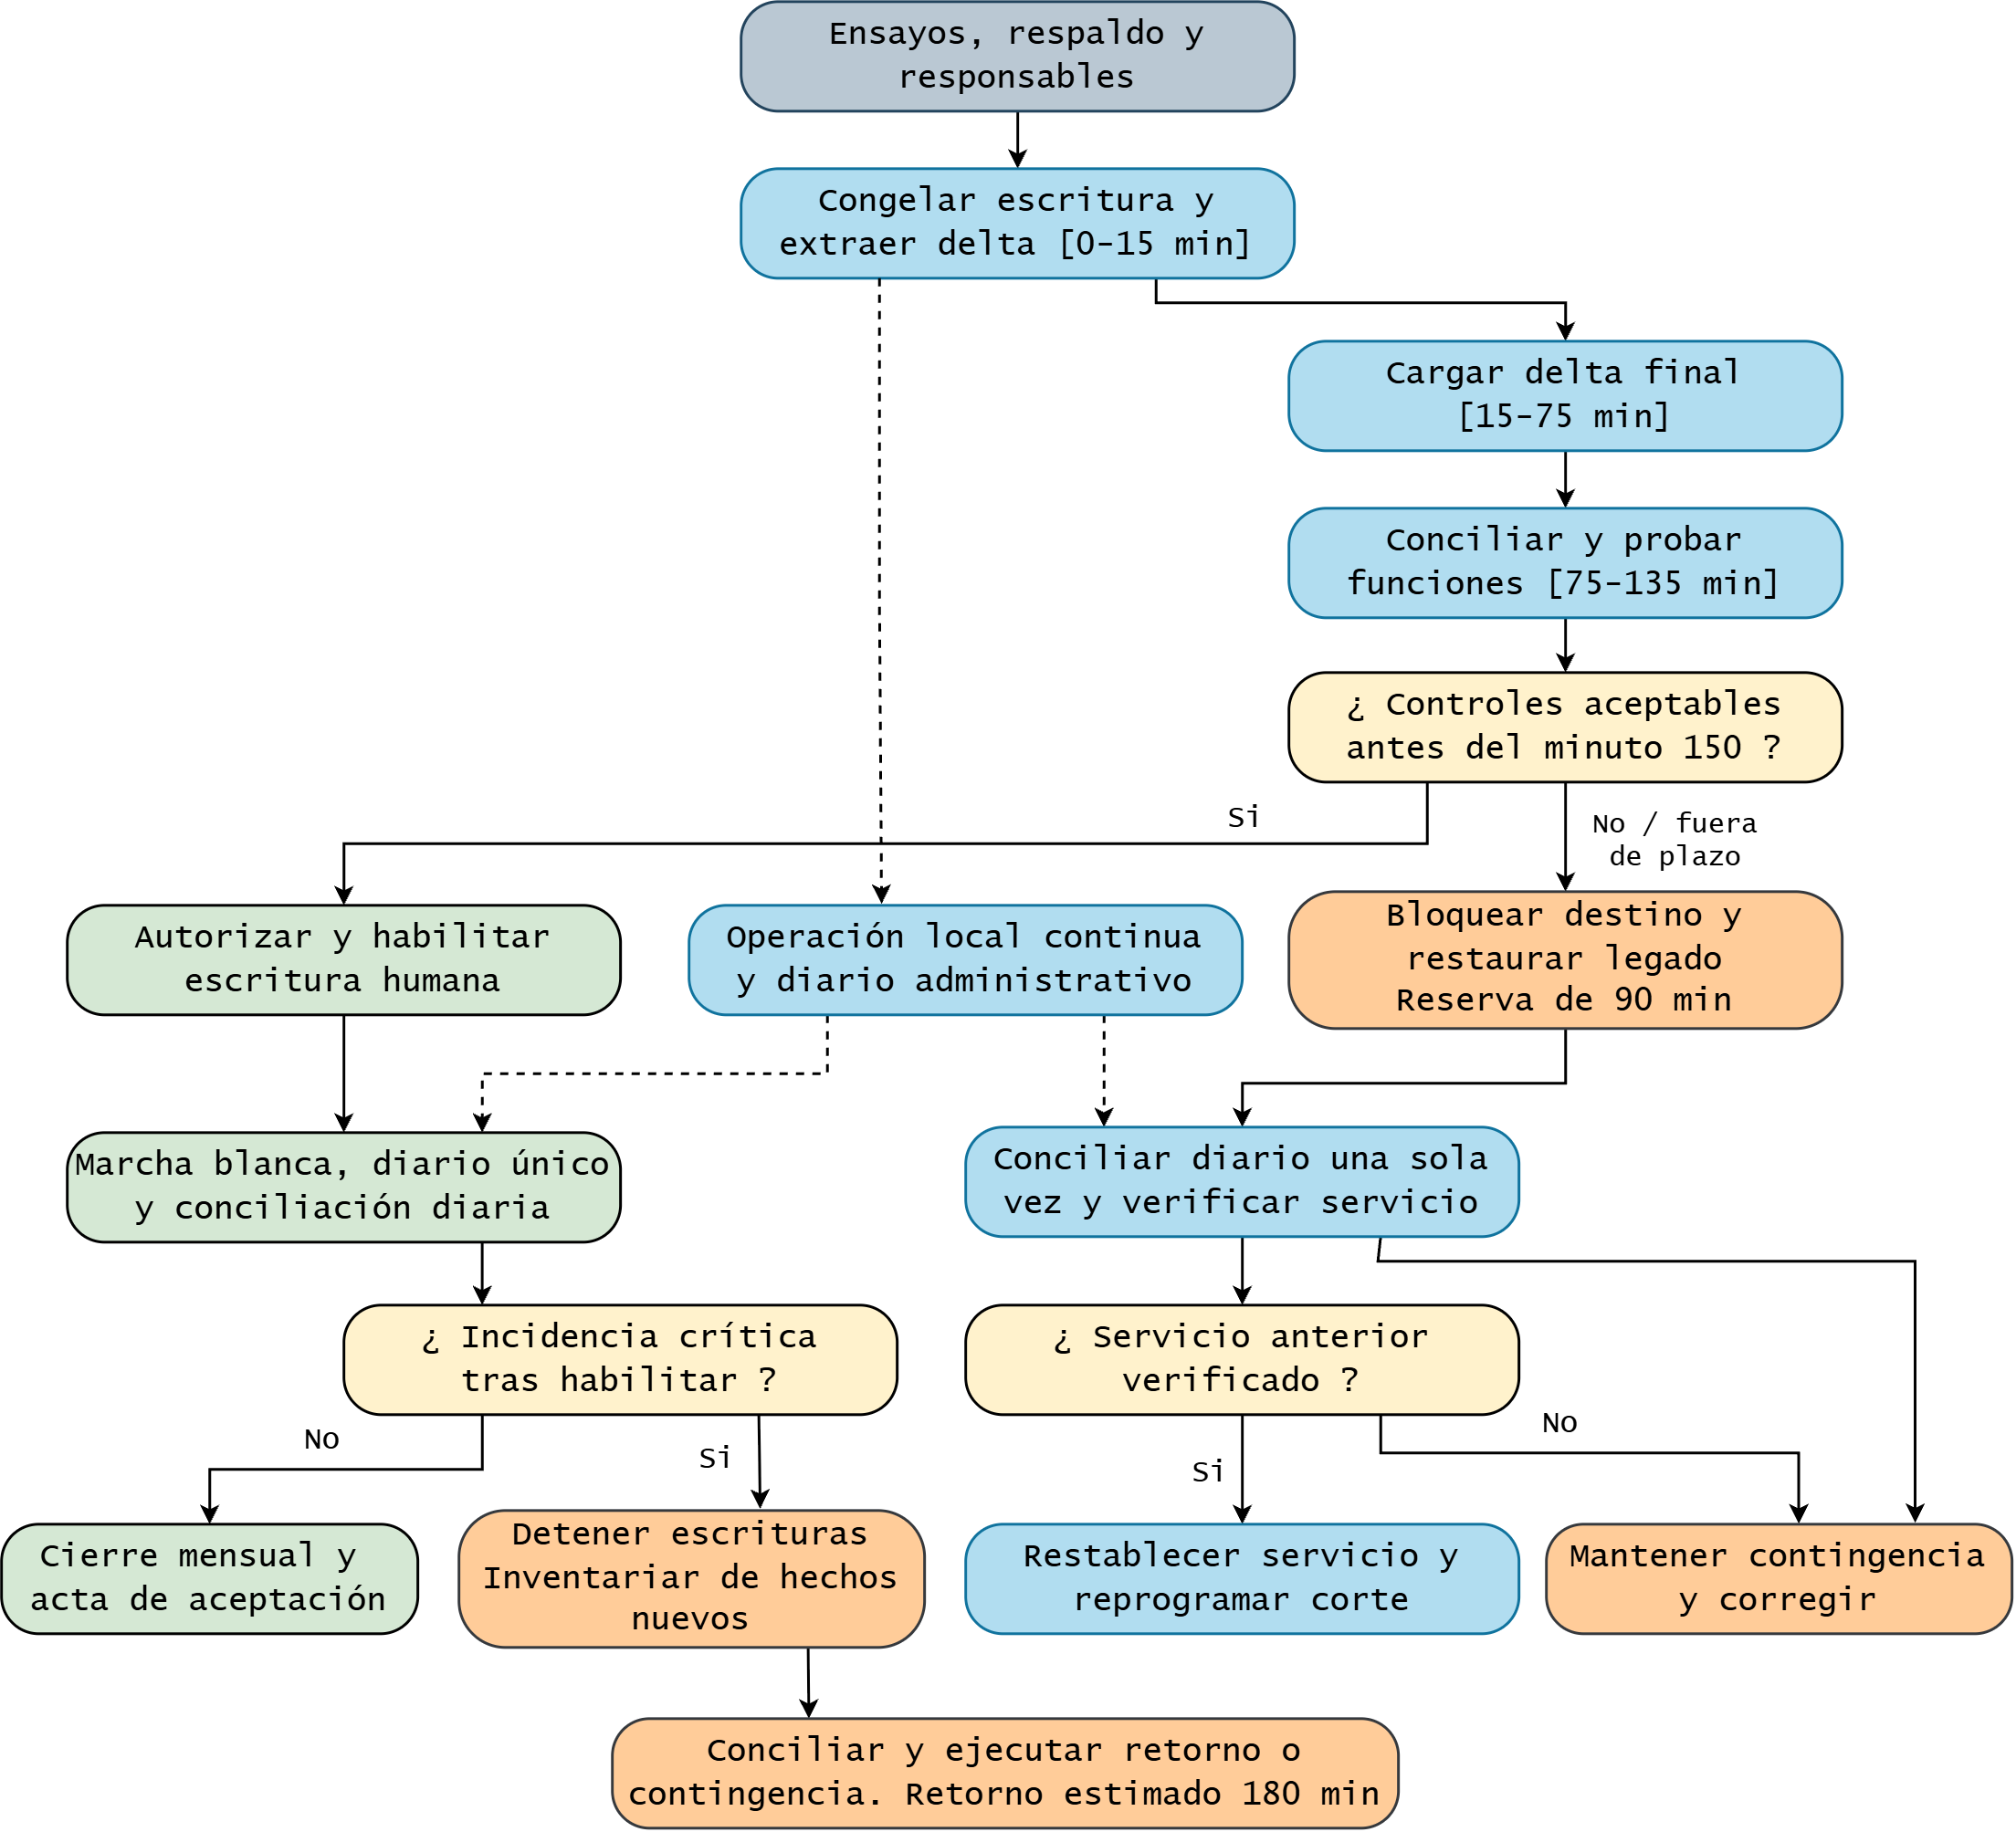
\includegraphics[width=\linewidth]{figuras/F5_16.png}
    }
    \caption{Decisión de continuidad o retorno}
    \label{fig:decision_corte}
    \FuenteFigura{PUCV (2026b, RT-05.11 y RT-20.02--RT-20.03).}
\end{figure}

\newpage
La escritura administrativa nueva permanecerá bloqueada hasta registrar la decisión de continuidad. Esta secuencia reduce el retorno previo a la habilitación a recuperar la autoridad anterior e incorporar el diario controlado. La ruta de aceptación inicia la marcha blanca; no elimina la obligación de revisar las diferencias del período posterior.

\textbf{Procedimiento de retorno:} antes del corte se conservarán la copia final del origen, la versión de la aplicación, el esquema de destino y las correspondencias de carga. Si se rechaza el paso antes de habilitar escrituras nuevas, se desactivarán los cargadores, se aislará el destino del corte y se restablecerá la escritura anterior. Se incorporará el diario una sola vez y se comprobarán saldos, consultas y acceso antes de declarar el servicio restablecido. Los datos del ensayo fallido se conservarán restringidos como evidencia.

Si ya existen operaciones nuevas, se detendrán las escrituras del dominio afectado y se inventariarán sus identificadores, efectos y respuestas externas. Se decidirá qué hechos pueden incorporarse al sistema anterior y cuáles deben mantenerse en el registro de contingencia conciliado. Nunca se restaurará una copia anterior descartando pagos, despachos u otros hechos posteriores. Un envío contable con resultado desconocido se consultará y conciliará antes de reintentarlo.

La reserva de 90 minutos se comprobará para el retorno antes de habilitar nuevas escrituras. Para el retorno administrativo posterior, con hechos nuevos desde el último cierre conciliado, se propone una estimación inicial de 180 minutos:
\begin{itemize}
    \item 15 minutos para aislar escrituras y delimitar el alcance.
    \item 45 minutos para inventariar las operaciones y contrastar sus respuestas externas.
    \item 60 minutos para incorporar los hechos representables en el legado y conciliar el diario.
    \item 60 minutos para incorporar los hechos representables en el legado y conciliar el diario.
\end{itemize}

Esta estimación presupone una copia recuperable, correspondencias de retorno probadas y disponibilidad del responsable técnico y del validador funcional. Se refiere al servicio administrativo afectado, la captura operacional del recinto continúa bajo su autoridad local.

Antes de habilitar la nueva escritura, se probará este escenario con el mayor volumen previsto de cambios administrativos, incluidos los reintentos y las respuestas contables pendientes. La prueba permitirá confirmar o ajustar el tiempo estimado y verificar su compatibilidad con el plan de implantación.

Si el sistema legado no puede registrar un hecho nuevo, no se logra conciliar un efecto externo o el retorno supera el tiempo previsto, el diario de contingencia se mantendrá como única autoridad de registro. En ese caso, se aplicará una corrección controlada, sin descartar operaciones ni repetir pagos o cargos. La jefatura del proyecto dejará registrada la decisión, junto con el responsable y el plazo de regularización. Los 180 minutos son una estimación de planificación de Synaptix. Ese tiempo aún no ha sido demostrado y no amplía la reserva de 90 minutos definida para el corte previo.

\textbf{Aceptación y cierre:} administración, Escuela y Operaciones registrarán sus conformidades por conjunto; Calidad entregará la evidencia de controles; y la gerencia autorizará el cambio de autoridad administrativa. El acta identificará alcance, versiones, fecha, resultados, incidencias no críticas admitidas y responsables de su tratamiento. Toda diferencia admitida tendrá explicación y plazo; una incidencia crítica no se trasladará al acta como una excepción de aceptación.

Durante la marcha blanca se compararán diariamente recuentos, movimientos, saldos y hechos facturables, incluyendo un cierre mensual completo con el suplente funcional. Se medirán también los tiempos de consulta y los indicadores de 5.4. Un defecto que altere custodia, autorización, saldo o integridad de los expedientes activará la suspensión del avance del grupo y su procedimiento de corrección o retorno.

El cierre técnico entregará los mapeos, correspondencias, manifiestos, reglas, actas, procedimientos de consulta histórica y evidencia de retorno. La retirada del acceso de escritura al legado será verificable. Su retirada definitiva dependerá de demostrar que la consulta histórica, la retención y la exportación siguen disponibles; no se ejecutará por el solo hecho de terminar una carga.


%---------------------------------------------
\newpage
\section{Estrategia de desempeño} %5.4
\label{sec:sd5_desempeno}
La estrategia de desempeño relaciona la carga del puerto con la capacidad de captura, persistencia, consulta y recuperación de la solución. Mantiene PostgreSQL 18, los repositorios documentales, la persistencia móvil y los almacenes derivados definidos en 5.2 y SD4. La selección de un motor o la existencia de una réplica no acreditan por sí solas que se cumplan los tiempos de respuesta.

Se distinguirán tres condiciones: los datos operacionales entregados por el caso, las hipótesis de diseño de Synaptix y los resultados medidos durante las pruebas. Las cifras de este apartado pertenecen a las dos primeras condiciones. La aceptación requerirá evidencias bajo carga y controles de integridad, conforme a las Bases Técnicas Transversales y a los umbrales particulares del caso (Pontificia Universidad Católica de Valparaíso [PUCV], 2026b, cap.~9; PUCV, 2026c, RT-03.10, RT-03.13, RT-05.29 y RT-09.01).

\subsection{Volumetría y carga}
\label{subsec:sd5_volumetria}

El dimensionamiento toma como referencia SD2, apartados 2.3 y 2.5 y anexo A2.7, y conserva las hipótesis de SD4, apartado 4.2. La base física comprende 320 amarras y 640 puntos de medición a instalar, uno de agua y otro de energía por amarra. La ampliación en evaluación comprende hasta 380 amarras y 760 puntos. Estos puntos representan el diseño de instrumentación; el caso informa que hoy no existe medición individual instalada.

El escenario operacional de concentración será el viernes de 07:00 a 11:00 descrito en C07, apartado 14.2: noventa zarpes, veinte recaladas, tres clases en el agua y actividad de varadero simultánea. Ese escenario se conservará completo en la prueba. La distribución anual del apartado 14.1 sirve para almacenamiento y crecimiento, pero no se utilizará para diluir esa concentración.

Además de la ampliación física, se verificará el crecimiento de al menos tres veces la volumetría inicial en tres años, exigido por BT RT-09.03. Para la instrumentación inicial de 640 puntos, el escenario de capacidad equivalente comprende 1.920 puntos. No representa una ampliación física acordada a 960 amarras; es una condición de escalabilidad que deberá satisfacerse mediante parametrización y aumento de recursos, sin cambiar el modelo de negocio.

\textbf{Transacciones, solicitudes y personas concurrentes:} una transacción de negocio es una actuación válida, como confirmar una asignación o registrar una salida. Una solicitud HTTP es una llamada a un servicio; un evento es la información publicada sobre una actuación; y una muestra es una lectura de un punto. Una sola transacción puede generar varias solicitudes, registros y eventos. Sus tasas se medirán por separado.

Se conservan 50 personas internas y 150 externas concurrentes como hipótesis de diseño. Las sesiones externas se distribuirán entre 60 armadores, 45 apoderados, 30 visitantes y 15 contratistas. Es una mezcla de prueba y no un recuento observado. La población mensual de 3.400 personas y la dotación de 78 trabajadores de temporada no se equiparan automáticamente a sesiones simultáneas.

Para hacer reproducible la tasa de negocio, se adopta en régimen normal una actuación por persona interna cada 20 segundos y una por persona externa cada 60 segundos. Para la carga máxima se adoptan intervalos de cinco y quince segundos, respectivamente:
\[
\lambda_{\mathrm{normal}}=\frac{50}{20}+\frac{150}{60}=5
\quad\mbox{transacciones/s},
\]
\[
\lambda_{\mathrm{maxima}}=\frac{50}{5}+\frac{150}{15}=20
\quad\mbox{transacciones/s}.
\]
Los intervalos son supuestos de actividad de Synaptix para construir una carga simultánea superior al promedio del puerto. Los flujos de la mañana crítica formarán parte de esa mezcla; no se sumarán nuevamente como si fueran otra población independiente. Las consultas, notificaciones y sincronización se identificarán como cargas adicionales.

Como supuesto de prueba se consideran cuatro llamadas de servicio por actuación, con cinco consultas adicionales por segundo en régimen normal y veinte en carga máxima. Así, \(5 \times 4 + 5 = 25\) solicitudes/s para régimen normal y \(20 \times 4 + 20 = 100\) solicitudes/s para carga máxima reproducen la capacidad inicial de referencia de SD4. El número real de llamadas por flujo se obtendrá de las trazas de la aplicación y sustituirá ese coeficiente antes de aceptar la capacidad.

La Tabla~\ref{tab:sd5_escenarios_carga} separa los escenarios que deben verificarse.

\begingroup
\setlength{\tabcolsep}{3pt}
\begin{longtable}{@{}L{.25\textwidth}L{.27\textwidth}L{.22\textwidth}L{\dimexpr.26\textwidth-18pt\relax}@{}}
\caption{Escenarios de transacciones y concurrencia}\label{tab:sd5_escenarios_carga}\\
\hline
\EncabezadoTabla{Escenario} & \EncabezadoTabla{Sesiones internas / externas} & \EncabezadoTabla{Transacciones/s} & \EncabezadoTabla{Solicitudes HTTP/s} \\ \hline
\endfirsthead
\hline
\EncabezadoTabla{Escenario} & \EncabezadoTabla{Sesiones internas / externas} & \EncabezadoTabla{Transacciones/s} & \EncabezadoTabla{Solicitudes HTTP/s} \\ \hline
\endhead
Régimen normal & 50 / 150 & 5 & 25 \\ \addlinespace \hline
Carga máxima & 50 / 150 & 20 & 100 \\ \addlinespace \hline
Carga de \(1{,}5\times\) & 75 / 225 & 30 & 150 \\ \addlinespace \hline
Estrés de portal & 50 / 300 & 30 & 140 \\ \addlinespace \hline
Crecimiento de \(3\times\) & 150 / 450 & 60 & 300 \\ \addlinespace \hline
\end{longtable}
\FuenteTabla{hipótesis de SD4; PUCV (2026b, RT-09.03 y RT-09.06); PUCV (2026c, sec.~14.2).}
\endgroup

La carga de \(1{,}5\times\) aumenta también las consultas adicionales, de veinte a treinta por segundo. El estrés de portal duplica únicamente las sesiones externas y mantiene las cincuenta internas y las veinte consultas adicionales; por eso su resultado es 140 solicitudes/s y no 150. Son pruebas diferentes y no intercambiables.

Las 100 solicitudes/s iniciales no demuestran cobertura del escenario de crecimiento de 300 solicitudes/s. La aplicación y la integración deberán escalar conforme a SD4 y verificarse con los mismos controles funcionales. La base de datos y el borde tendrán su propia medición de capacidad, porque ampliar tareas de aplicación no elimina una limitación de escritura o de almacenamiento.

\textbf{Captura y consolidación de telemetría:} la adquisición local se realizará cada minuto y la publicación de acumulados centrales cada quince minutos, conforme a SD4 DA-09 y 5.2.5. Cada registro conservará punto, instante, secuencia, calidad, época del contador y asociación vigente. Las muestras por minuto y los acumulados de quince minutos son poblaciones distintas.

Para \(P\) puntos se obtienen:
\[
N_{\mathrm{muestras/dia}}=P\times60\times24,\qquad
N_{\mathrm{consolidados/anio}}=P\times4\times24\times365.
\]
La Tabla~\ref{tab:sd5_volumen_telemetria} presenta el cálculo con un año de 365 días. Para tamaño se conservan los 300 bytes efectivos por registro consolidado de SD4; aplicar ese mismo tamaño a una muestra local es una hipótesis adicional de dimensionamiento, que se comprobará con el esquema real.

\begingroup
\setlength{\tabcolsep}{3pt}
\begin{longtable}{@{}L{.40\textwidth}L{.20\textwidth}L{.20\textwidth}L{\dimexpr.20\textwidth-18pt\relax}@{}}
\caption{Captura, consolidación y volumen de telemetría}\label{tab:sd5_volumen_telemetria}\\
\hline
\EncabezadoTabla{Indicador} & \EncabezadoTabla{640 puntos} & \EncabezadoTabla{760 puntos} & \EncabezadoTabla{1.920 puntos} \\ \hline
\endfirsthead
\hline
\EncabezadoTabla{Indicador} & \EncabezadoTabla{640 puntos} & \EncabezadoTabla{760 puntos} & \EncabezadoTabla{1.920 puntos} \\ \hline
\endhead
Muestras por día & 921.600 & 1.094.400 & 2.764.800 \\ \addlinespace \hline
Captura media local, muestras/s & 10,67 & 12,67 & 32,00 \\ \addlinespace \hline
Consolidados por día & 61.440 & 72.960 & 184.320 \\ \addlinespace \hline
Consolidados por año & 22.425.600 & 26.630.400 & 67.276.800 \\ \addlinespace \hline
Publicación media, registros/s & 0,71 & 0,84 & 2,13 \\ \addlinespace \hline
Muestras de 30 días, GB & 8,29 & 9,85 & 24,88 \\ \addlinespace \hline
Consolidados de un año, GB & 6,73 & 7,99 & 20,18 \\ \addlinespace \hline
Consolidados de cinco años, GB & 33,64 & 39,95 & 100,92 \\ \addlinespace \hline
\end{longtable}
\FuenteTabla{C07, sec.~14.1, SD4 DA-09 y BT RT-09.03; 300 bytes/registro como hipótesis de tamaño.}
\endgroup

La captura media de 12,67 muestras/s para 760 puntos no debe confundirse con la publicación central media de 0,84 registros/s. Si cada lote de 760 acumulados se distribuye durante sesenta segundos, la recepción de ese lote alcanza 12,67 registros/s. Para el servicio central se mantienen las capacidades de referencia de SD4 de 25 eventos/s sostenidos y 100 eventos/s en ráfaga; su margen debe comprobarse junto con los eventos de negocio.

Se escalonará la lectura entre concentradores y se conservará la secuencia de cada punto. Si todos los puntos producen su lectura al mismo instante, el borde puede recibir 760 muestras en una ráfaga local, aunque su promedio por minuto sea bajo. Esa ráfaga se probará separadamente; el límite de cien eventos/s del servicio central no es una explicación suficiente de la captura local. La adquisición no dependerá de que cada lectura se envíe inmediatamente a la nube.

El consumo por intervalo se reconstruirá desde acumulados, asociaciones y reglas de validación. Se probarán cambio de medidor, reinicio de contador, lecturas tardías y cambio de ocupante. La consolidación de quince minutos permite actualizar el consumo al menos cada hora, pero no acredita por sí sola que la atribución por amarra y contrato sea correcta.

\textbf{Reservas de almacenamiento:} se utilizarán GB decimales (\(10^9\) bytes), MB decimales (\(10^6\) bytes) y Mb/s para bits por segundo. Se separarán el dato lógico, los índices, la holgura, las proyecciones, las réplicas y los respaldos. Un recurso local redundante no duplicará la capacidad útil por el solo hecho de tener dos discos.

Para negocio sin telemetría se adopta un escenario de un millón de operaciones al año, cuatro registros de 1.000 bytes por operación y un factor de dos por índices y sobrecarga:
\[
V_{\mathrm{negocio}}=
\frac{1.000.000\times4\times1.000\times2}{10^9}
=8\ \mbox{GB/año}.
\]
Esta estimación incluye la auditoría básica de esas actuaciones. Se reservan 20~GB/año para incorporar maestros, versiones, rectificaciones y margen. El millón de operaciones es una hipótesis anual independiente de las tasas máximas de rendimiento; multiplicar veinte transacciones/s por todo el año sobrestimaría el volumen al suponer una carga máxima sostenida durante todo el año.

La Tabla~\ref{tab:sd5_reservas_datos} resume las reservas y sus límites. Las consultas sensibles adicionales y los eventos de seguridad se separan de la auditoría básica ya incluida. Para estimarlos se adopta un millón de consultas sensibles y 500.000 eventos de seguridad al año, de 1.000 bytes y factor de dos; son supuestos iniciales que se sustituirán por mediciones, sin omitir su retención.

\begingroup
\setlength{\tabcolsep}{3pt}
\begin{longtable}{@{}L{.26\textwidth}L{.29\textwidth}L{.20\textwidth}L{\dimexpr.25\textwidth-18pt\relax}@{}}
\caption{Reservas iniciales por familia de información}\label{tab:sd5_reservas_datos}\\
\hline
\EncabezadoTabla{Familia} & \EncabezadoTabla{Derivación o referencia} & \EncabezadoTabla{Reserva inicial} & \EncabezadoTabla{Límite del cálculo} \\ \hline
\endfirsthead
\hline
\EncabezadoTabla{Familia} & \EncabezadoTabla{Derivación o referencia} & \EncabezadoTabla{Reserva inicial} & \EncabezadoTabla{Límite del cálculo} \\ \hline
\endhead
Negocio y auditoría básica & 8 GB/año calculados & 20 GB/año & Sin telemetría ni accesos adicionales \\ \addlinespace \hline
Serie central & 7,99 GB/año; 760 puntos & 25 GB/año & Índices efectivos incluidos en 300 bytes \\ \addlinespace \hline
Documentos y versiones & 50.000 objetos/año de 2 MB & 100 GB/año & Sin video continuo \\ \addlinespace \hline
Consultas sensibles adicionales & 1 millón/año; 1.000 bytes; factor 2 & 2 GB/año & No incluye modificación ya contada \\ \addlinespace \hline
Eventos de seguridad & 500.000/año; 1.000 bytes, factor 2 & 1 GB/año & Sin duplicar auditoría de negocio \\ \addlinespace \hline
Cola local y evidencia & Hipótesis SD4 de 10 GB/día & 300 GB para 30 días & Sin sumar otra vez sus muestras \\ \addlinespace \hline
\end{longtable}
\FuenteTabla{hipótesis de SD4; 5.2.5; PUCV (2026b, RT-11.14 y RT-16.10); C07 RT-05.10.}
\endgroup

Los 100~GB documentales corresponden a objetos y versiones, no a 50.000 contratos. Las imágenes o documentos necesarios como evidencia se incluirán por su tamaño real. El video continuo permanecerá en la plataforma de cámaras según el alcance de SD4; una pieza exportada para un expediente sí pertenece al volumen documental. Duplicar el tamaño medio de objeto de 2 a 4~MB eleva esa reserva a 200~GB/año y se incluirá como sensibilidad.

La serie y el negocio reservan \(25+20=45\)~GB/año; cinco años representan 225~GB antes de otros componentes. Los 200~GB iniciales de SD4 son, por tanto, un punto de partida ampliable y no capacidad suficiente demostrada para toda la retención. Las consultas sensibles requieren al menos cinco años de auditoría cuando el caso no fija un plazo mayor; los eventos de seguridad conservan doce meses en línea y veinticuatro adicionales en archivo, conforme a BT RT-16.10 y RT-11.14.

Las proyecciones de lectura se dimensionarán por separado. Como estimación inicial, se consideran cuatro millones de filas resumidas de actividad del último año, 400 bytes por fila y factor de dos: 3,20~GB. Para 760 puntos se consideran resúmenes horarios de un año, (760\times24\times365=6.657.600) filas del mismo tamaño efectivo: 5,33~GB. Se añade un supuesto de 6.000 registros maestros y vigentes de 1.000 bytes y factor de dos: 0,012~GB. La suma es aproximadamente 8,54~GB; se propone reservar 15~GB iniciales para este almacén separado y probar el escenario equivalente de 45~GB al triplicar la carga. Los tamaños son hipótesis y no copias medidas del cliente.

Las proyecciones mantendrán la vista vigente y los conjuntos de consulta frecuente definidos en 5.2.3; no duplicarán necesariamente todo el historial. Los resúmenes no sustituyen la evidencia conservada en sus repositorios de origen. Las tablas e índices reales permitirán ajustar la reserva. Para cada repositorio se registrará:
\[
V_{\mathrm{fisico}}=
V_{\mathrm{datos}}+V_{\mathrm{indices}}+
V_{\mathrm{versiones}}+V_{\mathrm{holgura}}.
\]
El costo y la capacidad de réplicas y respaldos se calcularán además según sus copias y horizontes. Una copia mensual no se multiplicará por el tamaño final futuro como si todos los meses tuvieran la misma población.

La cola de 10~GB/día incluye las muestras y evidencia acumuladas para envío. Los 0,33~GB de muestras locales diarios de 760 puntos no se sumarán otra vez a esa misma cola; las copias efectivamente separadas sí se contabilizarán. Su reserva de 30 días no amplía el compromiso de operación autónoma de 24 horas: es margen de almacenamiento y conservación.

El crecimiento de al menos \(3\times\) se probará también en tamaño y consultas históricas, no solo en sesiones. La retención vigente y los bloqueos de expedientes determinarán qué información sigue activa. La revisión trimestral de capacidad comprobará el volumen real, el proyectado y el margen antes del siguiente ajuste, conforme a BT RT-09.09.

\subsection{Optimización del almacenamiento y consultas}
\label{subsec:sd5_optimizacion}

La optimización conservará las reglas de integridad y autoridad definidas en 5.1 y 5.2. Una respuesta rápida con un saldo antiguo o una asignación incompatible no será un resultado aceptable. Cada índice, partición o copia de consulta tendrá un uso concreto y una comprobación de su costo de lectura y escritura.

\textbf{Índices por consulta:} los índices se seleccionarán a partir del filtro, orden y volumen de las consultas frecuentes. PostgreSQL permite índices multicolumna; en un B-tree, las restricciones sobre las primeras columnas influyen en el tramo que debe recorrerse. Por ello se evaluarán combinaciones como entidad e instante, en vez de indexar cada atributo sin considerar su uso (PostgreSQL Global Development Group [PGDG], s.\,f.-c).

La Tabla~\ref{tab:sd5_indices_consulta} fija el conjunto inicial de accesos que se comprobará con datos representativos. Los campos se expresan por su significado funcional; sus nombres físicos se mantendrán alineados con el diccionario y las migraciones de esquema.

\begingroup
\setlength{\tabcolsep}{3pt}
\begin{longtable}{@{}L{.29\textwidth}L{.36\textwidth}L{\dimexpr.35\textwidth-12pt\relax}@{}}
\caption{Accesos e índices iniciales por patrón de consulta}\label{tab:sd5_indices_consulta}\\
\hline
\EncabezadoTabla{Consulta} & \EncabezadoTabla{Claves de acceso propuestas} & \EncabezadoTabla{Control asociado} \\ \hline
\endfirsthead
\hline
\EncabezadoTabla{Consulta} & \EncabezadoTabla{Claves de acceso propuestas} & \EncabezadoTabla{Control asociado} \\ \hline
\endhead
Último movimiento de nave & Embarcación, instante descendente & Estado y fuente del movimiento \\ \addlinespace \hline
Asignación vigente de puesto & Amarra, inicio; fin de vigencia & Exclusión de asignaciones incompatibles \\ \addlinespace \hline
Nómina y retiro de clase & Clase, estado, alumno & Entrega confirmada y versión \\ \addlinespace \hline
Consumo de un período & Medidor, instante, asociación & Intervalo y cambio de contador \\ \addlinespace \hline
Hechos por conciliar & Origen, estado de conciliación, fecha & Efecto externo y respuesta \\ \addlinespace \hline
Planes pendientes de cierre & Estado, vencimiento & Alerta desde el vencimiento \\ \addlinespace \hline
Consulta de auditoría & Entidad, instante, tipo de actuación & Permiso y retención \\ \addlinespace \hline
Deduplicación de recepción & Sistema emisor, identificador de evento & Unicidad de efecto \\ \addlinespace \hline
\end{longtable}
\FuenteTabla{5.1--5.2, SD4 DA-05/DA-08 y PGDG (s.\,f.-c, s.\,f.-e).}
\endgroup

El índice para encontrar una asignación no reemplazará la restricción que impide autorizar dos usos incompatibles del mismo puesto e intervalo. Esa validación permanecerá en la autoridad local. Tampoco se confirmará una entrega escolar a partir de una consulta cuya versión no incluya el retiro más reciente.

Los índices parciales se evaluarán para conjuntos reducidos y frecuentes, como planes abiertos o hechos pendientes de conciliación. Su condición deberá corresponder al filtro de las consultas que se pretende acelerar; no se asumirá que cualquier consulta aprovechará un índice parcial (PGDG, s.\,f.-e). Se medirán tamaño, costo de inserción y cambio de estado antes de incorporarlos.

Las consultas a atributos cifrados se apoyarán en identificadores técnicos y referencias autorizadas cuando corresponda. Un índice ordinario sobre un campo cifrado no se presentará como una búsqueda transparente por su valor original. Cualquier mecanismo adicional de búsqueda sobre información protegida deberá estar especificado en la política de seguridad y no debilitar su cifrado.

\textbf{Particionamiento temporal:} se conservarán particiones diarias para muestras locales por minuto y mensuales para los acumulados centrales. La auditoría se separará por familias de retención antes de aplicar cortes mensuales. Los maestros y las tablas pequeñas permanecerán sin particionar. La Tabla~\ref{tab:sd5_particiones} establece el criterio por conjunto.

\begingroup
\setlength{\tabcolsep}{3pt}
\begin{longtable}{@{}L{.25\textwidth}L{.20\textwidth}L{.21\textwidth}L{\dimexpr.34\textwidth-18pt\relax}@{}}
\caption{Organización temporal y condición de retiro}\label{tab:sd5_particiones}\\
\hline
\EncabezadoTabla{Conjunto} & \EncabezadoTabla{Organización} & \EncabezadoTabla{Clave temporal} & \EncabezadoTabla{Condición de retiro} \\ \hline
\endfirsthead
\hline
\EncabezadoTabla{Conjunto} & \EncabezadoTabla{Organización} & \EncabezadoTabla{Clave temporal} & \EncabezadoTabla{Condición de retiro} \\ \hline
\endhead
Muestras locales & Partición diaria & Instante de muestra & 30 días, base central comprobada \\ \addlinespace \hline
Acumulados centrales & Partición mensual & Inicio del intervalo & Cinco años, sin bloqueo vigente \\ \addlinespace \hline
Auditoría de negocio & Familia + mes & Instante de actuación & Retención aplicable a cada registro \\ \addlinespace \hline
Eventos de seguridad & Familia + mes & Instante del evento & 12 meses en línea + 24 en archivo \\ \addlinespace \hline
Maestros y vínculos & Sin partición inicial & No aplica & Vigencia y retención de categoría \\ \addlinespace \hline
\end{longtable}
\FuenteTabla{5.2.5; SD4 DA-09; PUCV (2026b, RT-11.14 y RT-16.10); C07 RT-05.10; PGDG (s.\,f.-d).}
\endgroup

Las consultas incluirán límites de tiempo que permitan descartar particiones ajenas al período solicitado. PostgreSQL soporta esa selección de particiones, pero su beneficio depende del filtro y del plan de ejecución, no se garantiza por la sola existencia de la división temporal (PGDG, s.\,f.-d).

La tarea administrada creará particiones anticipadamente y verificará su disponibilidad. Una muestra tardía se ubicará según su tiempo de origen, conservando el de recepción. Si su partición requiere recuperación o revisión de retención, se conservará en una cola identificada de incidencia hasta resolverla; no se descartará silenciosamente por no caber en la partición vigente.

La unicidad global de eventos se mantendrá en el registro de recepción y efectos de 5.2. Una restricción única sobre una tabla particionada debe incluir su clave de partición en los casos documentados por PostgreSQL; por tanto, una clave compuesta por fecha e identificador no se utilizará como prueba de que ese identificador nunca apareció en otra fecha (PGDG, s.\,f.-d). La deduplicación verificará emisor, identidad y contenido antes de aplicar el efecto.

El retiro de una partición se ejecutará después de comprobar retención, aceptación central y vínculos con incidencias o expedientes. Para muestras locales se conservarán las adicionales que respalden una rectificación abierta. Dividir por mes no permite eliminar un mes completo si contiene evidencia aún protegida.

\textbf{Consultas y separación de cargas:} las confirmaciones de negocio usarán el almacén transaccional de su dominio. Las vistas frecuentes se atenderán desde las proyecciones PostgreSQL separadas de 5.2.3 y los análisis históricos desde los conjuntos Parquet y Athena previstos en esa sección. Los informes amplios no compartirán el mismo recurso de escritura de la operación crítica.

Las consultas seleccionarán los atributos necesarios, usarán límites y paginación estable y evitarán repetir búsquedas de datos compartidos por cada fila del resultado. Los filtros por entidad, período y estado serán coherentes con sus índices. Las operaciones que retengan bloqueos se mantendrán breves y no esperarán una respuesta contable externa dentro de una transacción local.

Los lotes de carga, exportación y reconstrucción de proyecciones tendrán tamaños acotados, comprobación por lote y pausas para no desplazar las escrituras críticas. La tasa se ajustará con las pruebas. Se comprobará el mínimo transversal de 10.000 registros/minuto para procesamiento por lotes con registros representativos y validación activa, sin utilizar un lote vacío o una carga sin controles como evidencia.

La Figura~\ref{fig:rutas_desempeno} muestra las rutas que deben conservarse separadas.

\begin{figure}[htbp]
    \centering
    \makebox[\linewidth][c]{%
        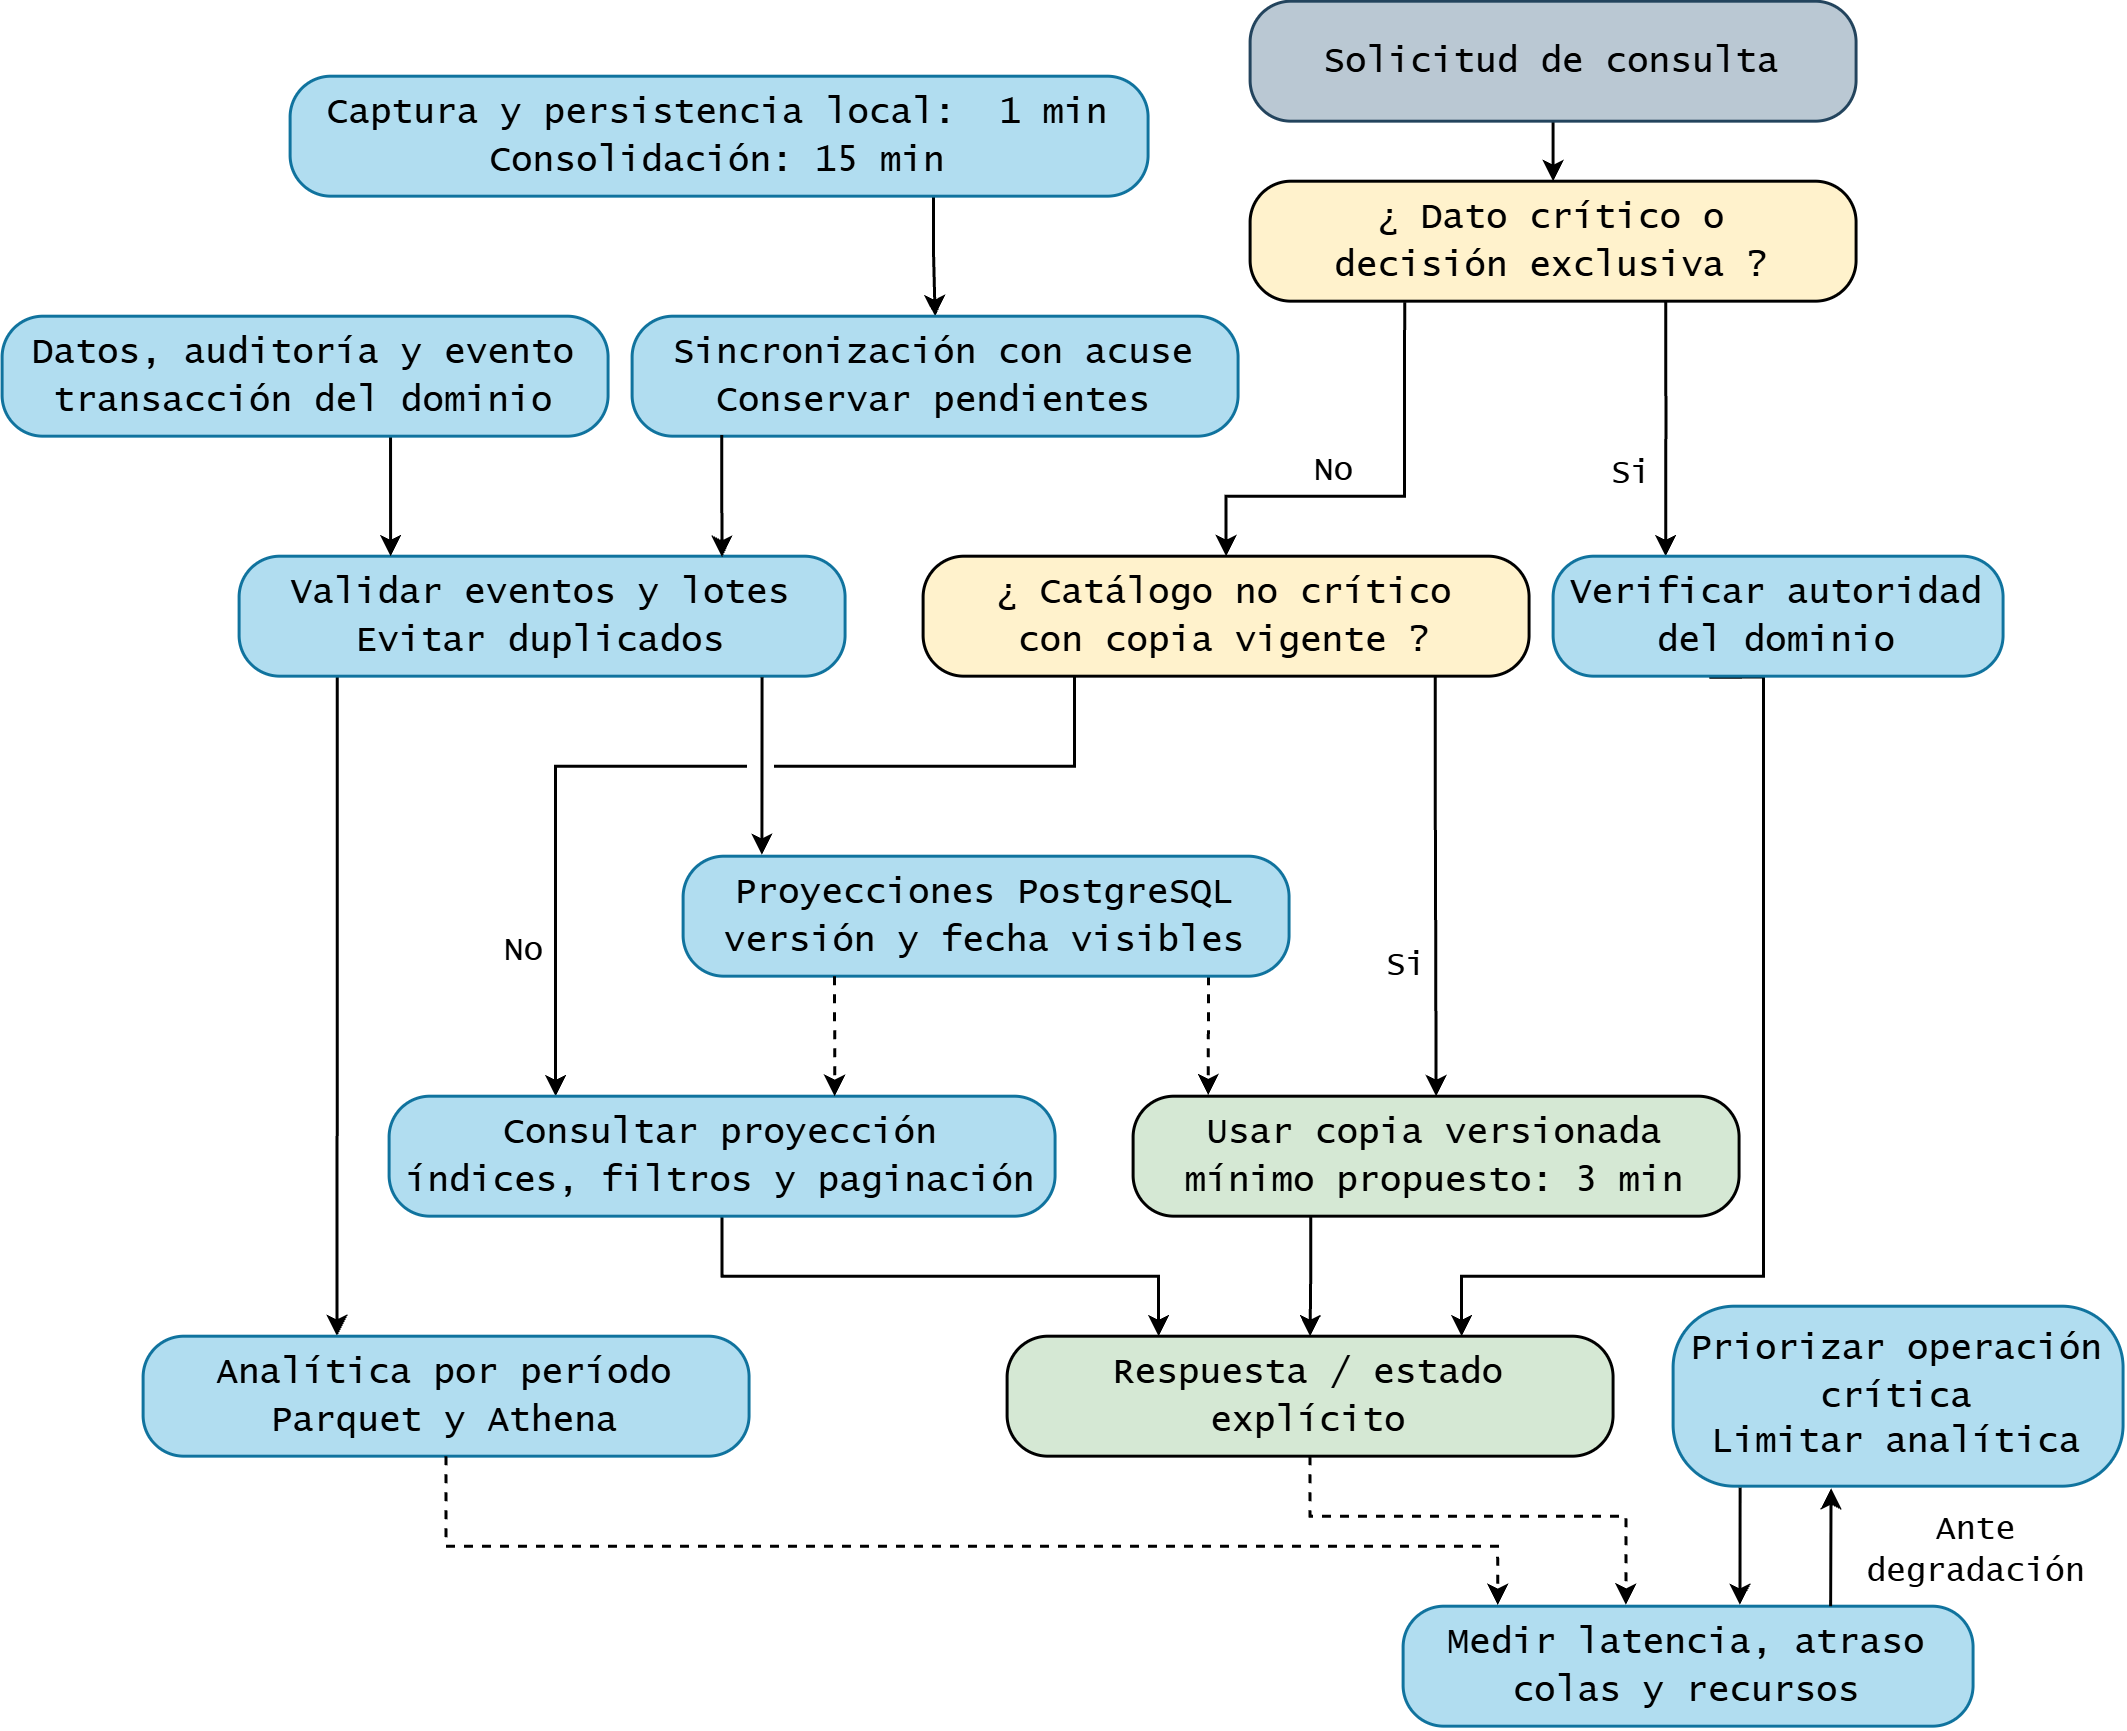
\includegraphics[width=0.9 \linewidth ]{figuras/F5_17.png}
    }
    \caption{Separación de confirmación, consulta frecuente y análisis histórico}
    \label{fig:rutas_desempeno}
    \FuenteFigura{5.2.3, SD4 DA-05/DA-08 y PUCV (2026b, RT-05.05).}
\end{figure}

Las flechas representan preparación de información derivada a partir de eventos y cargas controladas. Una proyección no escribe de vuelta el maestro ni es autoridad para una decisión exclusiva. Las cargas históricas pueden completar los conjuntos analíticos sin depender de que todo el historial permanezca en las proyecciones de consulta frecuente. El atraso y la versión serán visibles y la reconstrucción se ejecutará sin detener la captura.

\textbf{Caché y actualización:} se usarán las proyecciones y copias versionadas ya previstas, sin incorporar un nuevo servicio distribuido de caché. Los catálogos no críticos podrán reutilizarse durante un máximo propuesto de cinco minutos, con invalidación por versión. Ese plazo no se aplicará a ocupación, saldo, retiro escolar, permisos ni autorización de puesto.

La ocupación se actualizará por evento. Una vista con más de sesenta segundos desde el evento no se presentará como estado actualizado. El consumo se reconstruirá al menos cada hora desde los acumulados aceptados. Los indicadores ambientales se consolidarán diariamente. El saldo deberá obtenerse mediante la interfaz autorizada de su fuente contable, conservando fecha y estado de conciliación; un archivo periódico no acredita actualización en tiempo real.

La participación escolar y la entrega se comprobarán contra la autoridad operacional antes de confirmar una actuación incompatible. Ante falta de comunicación entre equipos, una cola local no demuestra estado compartido en tiempo real. La prueba incluirá la coordinación operacional definida en 5.2 y la verificación efectiva entre portería, escuela y monitor. Si ese flujo no mantiene la situación real exigida, no se considerará aceptado ni se reemplazará el umbral por una excepción de diseño.

Las copias sin conexión conservarán origen, versión, fecha y ámbito de autorización. Los permisos vencidos o una condición exclusiva indeterminada impedirán una confirmación automática. Se mantendrá la captura identificada y la coordinación segura del procedimiento correspondiente, sin convertir la disponibilidad de una copia en prueba de vigencia.

\textbf{Verificación de consultas:} se conservarán planes de ejecución antes y después de cada ajuste, con filas leídas, filas devueltas, particiones, tiempo y consumo de entrada/salida. \texttt{EXPLAIN} permite examinar el plan; su modalidad \texttt{ANALYZE} ejecuta la sentencia, por lo que el análisis de escrituras se realizará en preproducción con datos y controles apropiados (PGDG, s.\,f.-f). Un recorrido secuencial no será un defecto automático en una tabla pequeña; el criterio será su efecto medido sobre la carga representativa.

Los índices no utilizados y los que produzcan más costo de escritura que beneficio se revisarán antes de conservarlos. Las estadísticas y el mantenimiento de tablas se integrarán a la operación técnica de Synaptix. La marina no deberá administrar manualmente el motor para que los tiempos de respuesta se mantengan.

\subsection{Pruebas y monitoreo}
\label{subsec:sd5_pruebas_desempeno}

Las pruebas se ejecutarán sobre preproducción con el artefacto, las reglas y la configuración que se pretende liberar. Se utilizarán datos representativos y protegidos, el volumen histórico perfilado, series con la retención de diseño y documentos de varios tamaños. La infraestructura del generador de carga se separará de la solución para no atribuirle una saturación producida por el propio generador.

Se registrarán carga ofrecida, carga procesada, errores, rechazos controlados, percentiles 50/95/99, máximos, profundidad y antigüedad de colas, bloqueos, CPU, memoria, entrada/salida y tamaño. Los percentiles describen la distribución; los máximos y el número de incumplimientos comprobarán los límites expresos del caso. Un percentil 95 favorable no compensará una pérdida de registros o una asignación duplicada.

La Tabla~\ref{tab:sd5_plan_pruebas} fija la secuencia propuesta de pruebas. Las duraciones son reservas de ejecución del diseño y no resultados ya medidos.

\begingroup
\setlength{\tabcolsep}{3pt}
\begin{longtable}{@{}L{.24\textwidth}L{.31\textwidth}L{.17\textwidth}L{\dimexpr.28\textwidth-18pt\relax}@{}}
\caption{Escenarios de prueba y evidencia principal}\label{tab:sd5_plan_pruebas}\\
\hline
\EncabezadoTabla{Escenario} & \EncabezadoTabla{Carga o condición} & \EncabezadoTabla{Reserva} & \EncabezadoTabla{Evidencia principal} \\ \hline
\endfirsthead
\hline
\EncabezadoTabla{Escenario} & \EncabezadoTabla{Carga o condición} & \EncabezadoTabla{Reserva} & \EncabezadoTabla{Evidencia principal} \\ \hline
\endhead
Régimen y mañana crítica & 5 y 20 transacciones/s, flujos del caso & 1 h + 4 h & Tiempos por actuación y estados \\ \addlinespace \hline
Carga obligatoria \(1{,}5\times\) & 30 transacciones/s, 150 HTTP/s & 2 h & Umbrales y ausencia de pérdida \\ \addlinespace \hline
Estrés y saturación & 300 externos, aumento progresivo & Hasta identificar límite & Curva y recuperación de colas \\ \addlinespace \hline
Crecimiento \(3\times\) & Datos triples, 60 transacciones/s; 1.920 puntos & 2 h & Escalamiento sin rediseño \\ \addlinespace \hline
Ráfagas de medición & 760 muestras locales simultáneas, ráfagas centrales & Repetición por escenario & Secuencias, persistencia y acuses \\ \addlinespace \hline
Autonomía y reconexión & 24 h recinto, 12 h terreno; 8 h boyas & Cada horizonte completo & Manifiestos y convergencia \\ \addlinespace \hline
Restauración & Copia completa; claves, reglas y evidencia & Ensayo completo & Tiempo por dominio y funcionalidad \\ \addlinespace \hline
\end{longtable}
\FuenteTabla{PUCV (2026b, RT-09.03, RT-09.06--RT-09.07 y RT-07.12--RT-07.13); C07 RT-03.10/RT-03.13.}
\endgroup

Durante las pruebas de carga se mantendrán captura, consultas, notificaciones, procesamiento de eventos y analítica simultáneos. La prueba de \(1{,}5\times\) aumentará también las tasas centrales de telemetría de referencia a 37,5 eventos/s sostenidos y 150 en ráfaga; el generador conservará identidades distintas y contenido válido. Los reintentos duplicados se probarán como otro escenario y no se contarán como nuevos efectos.

El estrés identificará el punto de saturación mediante aumentos escalonados y comprobará la recuperación al reducir la carga. Se utilizarán el almacenamiento y la retención del escenario de crecimiento para probar consultas históricas. No bastará triplicar las sesiones sobre una base casi vacía. La prueba de un solo nodo local comprobará además que ese nodo sostiene el subconjunto crítico y conserva la reserva de SD4.

\textbf{Umbrales operacionales.} La Tabla~\ref{tab:sd5_umbral_caso} conserva los límites del caso y la frontera de medición de cada uno. Su trazabilidad funcional corresponde a RNF-DES-01--RNF-DES-11 y RNF-CONT-04 del anexo A2.2.

\begingroup
\setlength{\tabcolsep}{3pt}
\begin{longtable}{@{}L{.34\textwidth}L{.22\textwidth}L{\dimexpr.44\textwidth-12pt\relax}@{}}
\caption{Límites de aceptación del caso}\label{tab:sd5_umbral_caso}\\
\hline
\EncabezadoTabla{Proceso o información} & \EncabezadoTabla{Límite} & \EncabezadoTabla{Inicio y término de medición} \\ \hline
\endfirsthead
\hline
\EncabezadoTabla{Proceso o información} & \EncabezadoTabla{Límite} & \EncabezadoTabla{Inicio y término de medición} \\ \hline
\endhead
Asignación de amarra visitante & \(\leq45\) s & Consulta radial a confirmación \\ \addlinespace \hline
Registro de salida o regreso & \(\leq10\) s; dos interacciones & Inicio del registro a persistencia \\ \addlinespace \hline
Nómina y legajo de zarpe & \(\leq90\) s & Inicio del flujo a antecedentes conformados \\ \addlinespace \hline
Salida de clase, hasta 18 botes & \(\leq60\) s & Inicio a nómina completa persistida \\ \addlinespace \hline
Emergencia a 296 armadores & \(\leq10\) min & Activación a último envío \\ \addlinespace \hline
Plan vencido sin cierre & \(\leq15\) min & Vencimiento a generación de alerta \\ \addlinespace \hline
Ocupación de amarra & \(\leq60\) s & Ocurrencia del evento a vista actualizada \\ \addlinespace \hline
Consumo por amarra & Al menos horario & Datos de intervalo a acumulado actualizado \\ \addlinespace \hline
Saldo del armador & Tiempo real & Cambio confirmado a consulta vigente \\ \addlinespace \hline
Situación de escuela & Tiempo real, sin excepción & Hecho a situación efectiva compartida \\ \addlinespace \hline
Indicadores ambientales & Diario & Jornada a consolidación correspondiente \\ \addlinespace \hline
Reconexión tras 24 h & \(\leq30\) min & Enlace restituido a conciliación completa \\ \addlinespace \hline
\end{longtable}
\FuenteTabla{PUCV (2026c, RT-09.01, RT-05.29 y RT-03.13); anexo SD2 A2.2.}
\endgroup

Los tiempos de terreno incluyen la interacción de la persona y la persistencia del registro, en el momento seguro del procedimiento. Se comprobarán con operadores y dispositivos representativos; medir solo la llamada al servidor no verifica una asignación por radio ni la preparación de un zarpe. En ocupación se contará desde la ocurrencia del evento, incluyendo captura y transporte, no desde su digitación posterior.

Para planes vencidos no se añadirá una gracia de treinta minutos. La prueba de emergencia verificará los tres canales exigidos, sus destinatarios e intentos, y distinguirá último envío de entrega o acuse. Para saldo y escuela, las bases no fijan un número de segundos que autorice reemplazar \emph{tiempo real} por cinco minutos o sesenta segundos. Se comprobarán actualización por cambio y consulta contra la autoridad; la disponibilidad real de la integración contable y la coordinación local serán condiciones de aceptación.

También se conservarán los umbrales transversales de BT, apartado 9.1, mostrados en la Tabla~\ref{tab:sd5_umbral_bt}. Se medirán en el percentil 95 bajo carga máxima sobre la experiencia real de uso, salvo la capacidad de lotes que se mide como tasa.

\begingroup
\setlength{\tabcolsep}{3pt}
\begin{longtable}{@{}L{.47\textwidth}L{.23\textwidth}L{\dimexpr.30\textwidth-12pt\relax}@{}}
\caption{Umbrales transversales de respuesta y procesamiento}\label{tab:sd5_umbral_bt}\\
\hline
\EncabezadoTabla{Operación} & \EncabezadoTabla{Umbral} & \EncabezadoTabla{Tipo de comprobación} \\ \hline
\endfirsthead
\hline
\EncabezadoTabla{Operación} & \EncabezadoTabla{Umbral} & \EncabezadoTabla{Tipo de comprobación} \\ \hline
\endhead
Carga inicial del portal & 2 s & P95 extremo a extremo \\ \addlinespace \hline
Navegación entre vistas & 1 s & P95 con vistas cargadas \\ \addlinespace \hline
Consulta simple API & 500 ms & P95 de respuesta \\ \addlinespace \hline
Escritura transaccional API & 800 ms & P95 de respuesta \\ \addlinespace \hline
Búsqueda compuesta & 3 s & P95 de consulta \\ \addlinespace \hline
Informe estándar & 30 s & P95 hasta resultado \\ \addlinespace \hline
Procesamiento por lotes & \(\geq10.000\) registros/min & Tasa con validación activa \\ \addlinespace \hline
Archivo de 100 MB & 60 s & P95 de carga completa \\ \addlinespace \hline
Arranque en frío & 60 s & P95 hasta servicio utilizable \\ \addlinespace \hline
\end{longtable}
\FuenteTabla{PUCV (2026b, sec.~9.1); anexo SD2 A2.2, RNF-DES-12.}
\endgroup

Las condiciones de la prueba identificarán acceso, dispositivo, tamaño de archivo y recorrido de la solicitud. Se registrarán los relojes y su incertidumbre para correlacionar captura, recepción y visualización. Si la incertidumbre impide comprobar un límite, ese resultado no se utilizará para declarar el control aprobado.

\textbf{Sincronización después de desconexión:} se aislará el recinto del exterior durante 24 horas y se ejecutarán recepción, asignación de amarra, salidas, regresos, preparación de zarpe, combustible y escuela. Se probarán además dispositivos de terreno durante doce horas y la inspección de boyas durante ocho, verificando consulta local, permisos, batería y persistencia. No se reducirá la prueba a autonomía eléctrica.

La reconexión se ejecutará con nuevas operaciones concurrentes, reintentos, mensajes desordenados, reinicio del proceso y pérdida de acuse después de una confirmación. El cronómetro comenzará al restablecerse efectivamente el enlace. La aceptación exigirá igualdad de conjuntos de identificadores, secuencias conciliadas, cero efectos duplicados y ausencia de pérdida en todos los registros exigidos.

Para un lote de 10~GB y 50~Mb/s efectivos dedicados:
\[
t_{\mathrm{transferencia}}=
\frac{10\times10^9\times8}{50\times10^6}
=1.600\ \mbox{s}=26\ \mbox{min}\ 40\ \mbox{s}.
\]
Una sensibilidad de 20~\% adicional eleva ese tiempo a 32 minutos. A 100~Mb/s efectivos, el mismo cálculo entrega 13 minutos 20 segundos y 16 minutos con el factor adicional. El factor es una hipótesis de sensibilidad, no una medición de protocolo ni una garantía de procesamiento.

Para que esa sensibilidad de 10~GB quepa en treinta minutos se requieren al menos 53,34~Mb/s efectivos dedicados, redondeando hacia arriba. Esa cifra todavía debe considerar tráfico nuevo y la distribución real entre transferencia, validación y persistencia. Por lo tanto, el respaldo de 50~Mb/s no acredita el compromiso por aritmética ideal. La prueba medirá el caudal disponible y el tiempo completo por el enlace principal y por el de respaldo.

Se priorizarán los registros críticos, sin excluir silenciosamente documentos necesarios para comprobar su integridad. El manifiesto distinguirá recepción durable, aceptación de negocio y archivo íntegro. No se declarará sincronización completa mientras existan registros o evidencias que pertenezcan al conjunto obligatorio sin conciliar. Si el ensayo excede treinta minutos, se ajustarán el volumen transportado dentro de sus reglas de integridad, la precarga de referencias o la capacidad del enlace antes de autorizar la operación.

\textbf{Estimación y prueba de restauración por dominio:} la recuperación se comprobará con datos, claves, documentos, índices, permisos y reaplicación de eliminaciones o revocaciones. El objetivo regional de SD4 es de cuatro horas; no equivale al tiempo ya medido de restaurar cualquier volumen.

Para contar con una estimación inicial por dominio, se distribuye exclusivamente el volumen histórico provisional de 10~GB estructurados y 50~GB documentales de 5.3. Las proporciones de la Tabla~\ref{tab:sd5_restauracion_dominios} son supuestos de reparto de Synaptix, no inventario del cliente. Se reemplazarán con los tamaños perfilados y con la población acumulada que deba recuperarse en cada prueba.

\begingroup
\setlength{\tabcolsep}{3pt}
\begin{longtable}{@{}L{.39\textwidth}L{.20\textwidth}L{.20\textwidth}L{\dimexpr.21\textwidth-18pt\relax}@{}}
\caption{Estimación inicial de restauración por dominio}\label{tab:sd5_restauracion_dominios}\\
\hline
\EncabezadoTabla{Dominio} & \EncabezadoTabla{Datos estructurados, GB} & \EncabezadoTabla{Documentos, GB} & \EncabezadoTabla{Tiempo estimado, min} \\ \hline
\endfirsthead
\hline
\EncabezadoTabla{Dominio} & \EncabezadoTabla{Datos estructurados, GB} & \EncabezadoTabla{Documentos, GB} & \EncabezadoTabla{Tiempo estimado, min} \\ \hline
\endhead
Clientes y contratos & 2,0 & 10,0 & 74 \\ \addlinespace \hline
Operación marítima & 0,8 & 4,0 & 54 \\ \addlinespace \hline
Escuela náutica & 1,2 & 10,0 & 71 \\ \addlinespace \hline
Varadero y contratistas & 0,8 & 8,0 & 65 \\ \addlinespace \hline
Combustible & 0,3 & 2,0 & 47 \\ \addlinespace \hline
Ambiente y consumos & 0,7 & 4,0 & 54 \\ \addlinespace \hline
Finanzas y cobranza & 2,5 & 8,0 & 71 \\ \addlinespace \hline
Infraestructura & 0,7 & 3,0 & 51 \\ \addlinespace \hline
Auditoría y seguridad & 1,0 & 1,0 & 47 \\ \addlinespace \hline
Total de volumen & 10,0 & 50,0 & Sin sumar tiempos individuales \\ \addlinespace \hline
\end{longtable}
\FuenteTabla{5.3; metodología conforme a PUCV (2026b, RT-07.13); no son tiempos medidos.}
\endgroup

El cálculo de cada dominio supone 6,25~MB/s de transferencia efectiva, equivalentes a 50~Mb/s; 20~MB/s efectivos para restaurar datos estructurados, incluidos sus índices; quince minutos de preparación; diez de reaplicación de registros de cambios y permisos; y quince de verificación funcional. Todos esos valores son hipótesis. Sean \(V_{s,i}\) el volumen estructurado y \(V_{d,i}\) el documental del dominio. Se redondea el resultado al minuto superior:
\[
t_i=15+
\frac{(V_{s,i}+V_{d,i})\times1.000}{6{,}25\times60}
+\frac{V_{s,i}\times1.000}{20\times60}
+10+15.
\]
Los volúmenes se expresan en GB decimales y el resultado en minutos. Las transferencias y comprobaciones incluyen los objetos; la mera recuperación de tablas no acredita un expediente disponible.

En todos los dominios se conserva el respaldo diario propuesto en 5.2.5, con recuperación a un punto en el tiempo de 35 días en nube y doce copias mensuales para recuperación. El subconjunto local usa copia diaria de treinta días. La retención documental permanece por categoría y no se reduce a la rotación de respaldo. La prueba mensual comprobará el tiempo efectivo sobre una muestra representativa y se ejecutará una restauración integrada antes de producción, conforme a BT RT-07.12.

Los tiempos individuales incluyen preparaciones repetidas y no deben sumarse para estimar la recuperación conjunta. Para ese volumen completo se cuenta una sola preparación, transferencia de 60~GB, restauración de 10~GB estructurados, diez minutos de reaplicación y cuarenta de comprobación integrada:
\[
t_{\mathrm{integrado}}=
15+\frac{60\times1.000}{6{,}25\times60}
+\frac{10\times1.000}{20\times60}+10+40
=233{,}33\ \mbox{min}.
\]
Son aproximadamente tres horas, 53 minutos y 20 segundos. El margen de seis minutos y cuarenta segundos frente a cuatro horas es reducido; duplicar el volumen eleva la estimación a 401,67 minutos, unas seis horas y 42 minutos con redondeo superior. Este escenario no acredita el RTO regional.

La recuperación regional prevista en SD4 utiliza réplicas y evidencia disponibles en el sitio secundario; restaurar desde cero es un escenario distinto. Se ensayarán ambos y se comprobará qué datos ya están disponibles, su atraso, las claves, la promoción y el acceso funcional. Si la restauración exigida no cabe en su objetivo, se ajustarán la capacidad de lectura, transferencia y escritura y la preparación de las copias antes de liberar el servicio. Las estimaciones por dominio se actualizarán con volumen real y crecimiento; el volumen histórico inicial no es un límite permanente.

\textbf{Monitoreo y respuesta:} se utilizarán la observabilidad y las trazas previstas en SD4, con correlación entre evento, solicitud, lote y efecto. Se registrará la antigüedad del dato visible, además del tiempo de respuesta HTTP. La primera limitación esperable de la base transaccional es la escritura y entrada/salida compartida entre índices, auditoría y consumo; es una hipótesis que se confirmará con la curva de carga, no un cuello de botella ya observado.

La Tabla~\ref{tab:sd5_monitoreo} fija umbrales iniciales de acción. Las alertas anticipadas son decisiones de operación de Synaptix y no reemplazan los límites de aceptación.

\begingroup
\setlength{\tabcolsep}{3pt}
\begin{longtable}{@{}L{.28\textwidth}L{.30\textwidth}L{\dimexpr.42\textwidth-12pt\relax}@{}}
\caption{Monitoreo y acciones ante degradación}\label{tab:sd5_monitoreo}\\
\hline
\EncabezadoTabla{Indicador} & \EncabezadoTabla{Umbral inicial} & \EncabezadoTabla{Acción} \\ \hline
\endfirsthead
\hline
\EncabezadoTabla{Indicador} & \EncabezadoTabla{Umbral inicial} & \EncabezadoTabla{Acción} \\ \hline
\endhead
Ocupación visible & Advertencia a 45 s; incumplimiento a 60 s & Revisar captura, cola y proyección \\ \addlinespace \hline
Consumo por amarra & Advertencia sin actualización en 45 min & Revisar secuencias y consolidación \\ \addlinespace \hline
Plan sin cierre & Advertencia al vencer; límite de 15 min & Priorizar generación y escalar falla \\ \addlinespace \hline
Recursos en nube & Más de 70\% durante 5 min & Escalar recurso; limitar tareas no críticas \\ \addlinespace \hline
Nodo local único & Más de 60\% durante carga crítica & Corregir capacidad para conservar 40\% libre \\ \addlinespace \hline
Almacenamiento & Uso proyectado superior a 70\% & Ampliar antes del agotamiento \\ \addlinespace \hline
Efectos y conciliación & Cualquier pérdida o duplicación & Detener efecto afectado y recuperar \\ \addlinespace \hline
Escuela y saldo & Dato vigente no comprobable & Consultar autoridad y activar tratamiento \\ \addlinespace \hline
\end{longtable}
\FuenteTabla{Reservas de SD4; C07 RT-05.29/RT-09.01; PUCV (2026b, RT-09.08--RT-09.09).}
\endgroup

Las proyecciones de escuela y saldo se supervisarán por versión y continuidad del flujo de cambios, sin asignarles una caducidad que rebaje el tiempo real. La indisponibilidad de su autoridad se declarará explícitamente y se atenderá mediante el procedimiento correspondiente. Un dato antiguo no se presentará como confirmado para mantener artificialmente un buen indicador de respuesta.

Para aplicación e integración se propone que la capacidad adicional quede utilizable dentro de sesenta segundos desde el umbral de escalamiento. El ensayo medirá detección, provisión y servicio efectivo; el arranque en frío de un componente no equivale por sí solo al tiempo total. Las colas conservarán los eventos durante esa transición y sus límites de edad se comprobarán contra cada proceso.

En el recinto, la conmutación o ampliación no deberá exigir al cliente administrar PostgreSQL. Si un nodo no conserva el 40~\% de reserva bajo la carga crítica, se ajustará su capacidad antes de producción. El umbral de 70~\% de nube no se aplicará al nodo local como si cumpliera esa reserva. En el servicio central se revisarán por separado CPU, memoria, conexiones y entrada/salida, sin deducir capacidad de una sola métrica.

Al superar la capacidad se limitarán consultas históricas y exportaciones no urgentes, se acotarán las tasas y se conservarán las solicitudes aceptadas con estado identificable. Los procesos críticos tendrán prioridad sin omitir validaciones. La persona recibirá un estado explícito de espera o rechazo; no se confirmará una actuación que solo está en cola ni se perderá silenciosamente una transacción (PUCV, 2026b, RT-09.08).

El responsable técnico de Synaptix mantendrá el monitoreo y las acciones de recuperación; Calidad revisará las pruebas; y Operaciones, Escuela y Administración comprobarán los resultados de sus flujos. Cada informe conservará entorno, versiones, población, carga, tiempos, errores, curva de saturación, recuperación y decisiones. La aceptación se trazará con A2.2, T-12 y el protocolo de pruebas, y la memoria de capacidad se organizará para A5.4.

Antes de cada paso a producción deberán aprobarse los escenarios aplicables, incluidos \(1{,}5\times\), crecimiento, continuidad y recuperación. Los defectos que afecten los límites críticos o la integridad impedirán la aceptación. Durante la operación se revisará trimestralmente la capacidad y después de cualquier cambio material de esquema, volumen, retención, integración o infraestructura se repetirán las pruebas afectadas.